\documentclass[11pt,oneside]{article}

\usepackage[letterpaper,top=0.78in,bottom=0.82in,left=0.82in,right=0.82in]{geometry}
\usepackage[T1]{fontenc}
\usepackage[utf8]{inputenc}
\usepackage{lmodern}
\usepackage{microtype}
\usepackage{graphicx}
\usepackage{booktabs}
\usepackage{longtable}
\usepackage{tabularx}
\usepackage{array}
\usepackage{enumitem}
\usepackage{xcolor}
\usepackage{listings}
\usepackage{fancyhdr}
\usepackage{titlesec}
\usepackage{hyperref}
\usepackage{tikz}
\usetikzlibrary{arrows.meta,positioning,fit,shapes.geometric}
\usepackage[most]{tcolorbox}
\usepackage{lastpage}
\usepackage{caption}
\usepackage{float}
\usepackage{pdflscape}
\usepackage{seqsplit}
\usepackage{needspace}

\definecolor{OInk}{HTML}{101827}
\definecolor{ONavy}{HTML}{172554}
\definecolor{OBlue}{HTML}{3B82F6}
\definecolor{OPurple}{HTML}{7C3AED}
\definecolor{OCyan}{HTML}{0891B2}
\definecolor{OGreen}{HTML}{047857}
\definecolor{ORed}{HTML}{B42318}
\definecolor{OAmber}{HTML}{B45309}
\definecolor{OSlate}{HTML}{475569}
\definecolor{OLight}{HTML}{F5F7FB}
\definecolor{OLine}{HTML}{D8DEEA}
\definecolor{OCode}{HTML}{111827}

\hypersetup{
  colorlinks=true,
  linkcolor=ONavy,
  urlcolor=OBlue,
  citecolor=OPurple,
  pdfauthor={Lee Daghlar Ostadi},
  pdftitle={Ostadix-lang: Structural Polyglot Orchestration, Native O-core, and World Execution},
  pdfsubject={Creator-authored technical whitepaper for Ostadix-lang 0.4.0 Unreleased at 36787b16},
  pdfkeywords={Ostadix-lang, O-lang, O-core, OIR, HGraph, polyglot programming}
}

\setlength{\parindent}{0pt}
\setlength{\parskip}{5.5pt plus 1pt minus 1pt}
\setlist[itemize]{leftmargin=1.35em,itemsep=2pt,topsep=3pt}
\setlist[enumerate]{leftmargin=1.55em,itemsep=2pt,topsep=3pt}
\renewcommand{\arraystretch}{1.18}
\setcounter{tocdepth}{2}

\titleformat{\section}
  {\Large\bfseries\color{ONavy}}
  {\thesection}{0.65em}{}
  [\vspace{-0.35em}\color{OLine}\titlerule]
\titleformat{\subsection}
  {\large\bfseries\color{OInk}}
  {\thesubsection}{0.55em}{}
\titleformat{\subsubsection}
  {\normalsize\bfseries\color{OPurple}}
  {\thesubsubsection}{0.5em}{}

\pagestyle{fancy}
\fancyhf{}
\fancyhead[L]{\small\color{OSlate}Ostadix-lang Technical Whitepaper}
\fancyhead[R]{\small\color{OSlate}\texttt{0.4.0 Unreleased / 36787b16}}
\fancyfoot[L]{\small\color{OSlate}Lee Daghlar Ostadi}
\fancyfoot[R]{\small\color{OSlate}\thepage\ /\ \pageref{LastPage}}
\renewcommand{\headrulewidth}{0.3pt}
\renewcommand{\footrulewidth}{0pt}

\lstdefinelanguage{Ostadix}{
  morekeywords={let,now,lazy,autonomous,batch,all,any,race,instantiate,realise,activate,dry_activate,current_system},
  sensitive=true,
  morecomment=[l]{\#},
  morestring=[b]"
}
\lstdefinestyle{ostyle}{
  language=Ostadix,
  backgroundcolor=\color{OCode},
  basicstyle=\ttfamily\small\color{white},
  keywordstyle=\bfseries\color{cyan!75},
  commentstyle=\itshape\color{green!55},
  stringstyle=\color{orange!72},
  frame=single,
  rulecolor=\color{ONavy},
  framesep=7pt,
  xleftmargin=0.02\linewidth,
  xrightmargin=0.02\linewidth,
  breaklines=true,
  breakatwhitespace=false,
  showstringspaces=false,
  columns=fullflexible,
  keepspaces=true,
  tabsize=2
}
\lstdefinestyle{plaincode}{
  backgroundcolor=\color{OLight},
  basicstyle=\ttfamily\small\color{OInk},
  frame=single,
  rulecolor=\color{OLine},
  framesep=6pt,
  breaklines=true,
  showstringspaces=false,
  columns=fullflexible,
  keepspaces=true
}

\newcommand{\product}{\textsc{Ostadix-lang}}
\newcommand{\ovalue}{\textsc{OValue}}
\newcommand{\oir}{\textsc{OIR}}
\newcommand{\hgraph}{\textsc{HGraph}}
\newcommand{\ocore}{\textsc{O-core}}
\newcommand{\src}[2]{\textcolor{OSlate}{\scriptsize[\path{#1}, lines #2]}\allowbreak}
\newcommand{\status}[2]{\textbf{\textcolor{#1}{#2}}}
\newcommand{\breakcode}[1]{\texttt{\seqsplit{#1}}}
\newcolumntype{P}[1]{>{\raggedright\arraybackslash}p{#1}}

\newtcolorbox{claimbox}[1][]{
  enhanced,colback=OLight,colframe=OBlue,boxrule=0.7pt,arc=2pt,
  left=8pt,right=8pt,top=7pt,bottom=7pt,
  title={#1},fonttitle=\bfseries\color{ONavy},coltitle=ONavy
}
\begin{document}
\hypersetup{pageanchor=false}

\begin{titlepage}
\thispagestyle{empty}
\begin{tikzpicture}[remember picture,overlay]
  \fill[OInk] (current page.south west) rectangle (current page.north east);
  \fill[OBlue] (current page.north west) rectangle ([yshift=-0.13in]current page.north east);
  \fill[OPurple] ([yshift=0.13in]current page.south west) rectangle (current page.south east);
  \draw[OBlue,line width=1.5pt,opacity=0.7]
    ([xshift=0.62in,yshift=-0.62in]current page.north west)
    rectangle
    ([xshift=-0.62in,yshift=0.62in]current page.south east);
\end{tikzpicture}

\color{white}
\vspace*{0.16in}
\begin{center}
  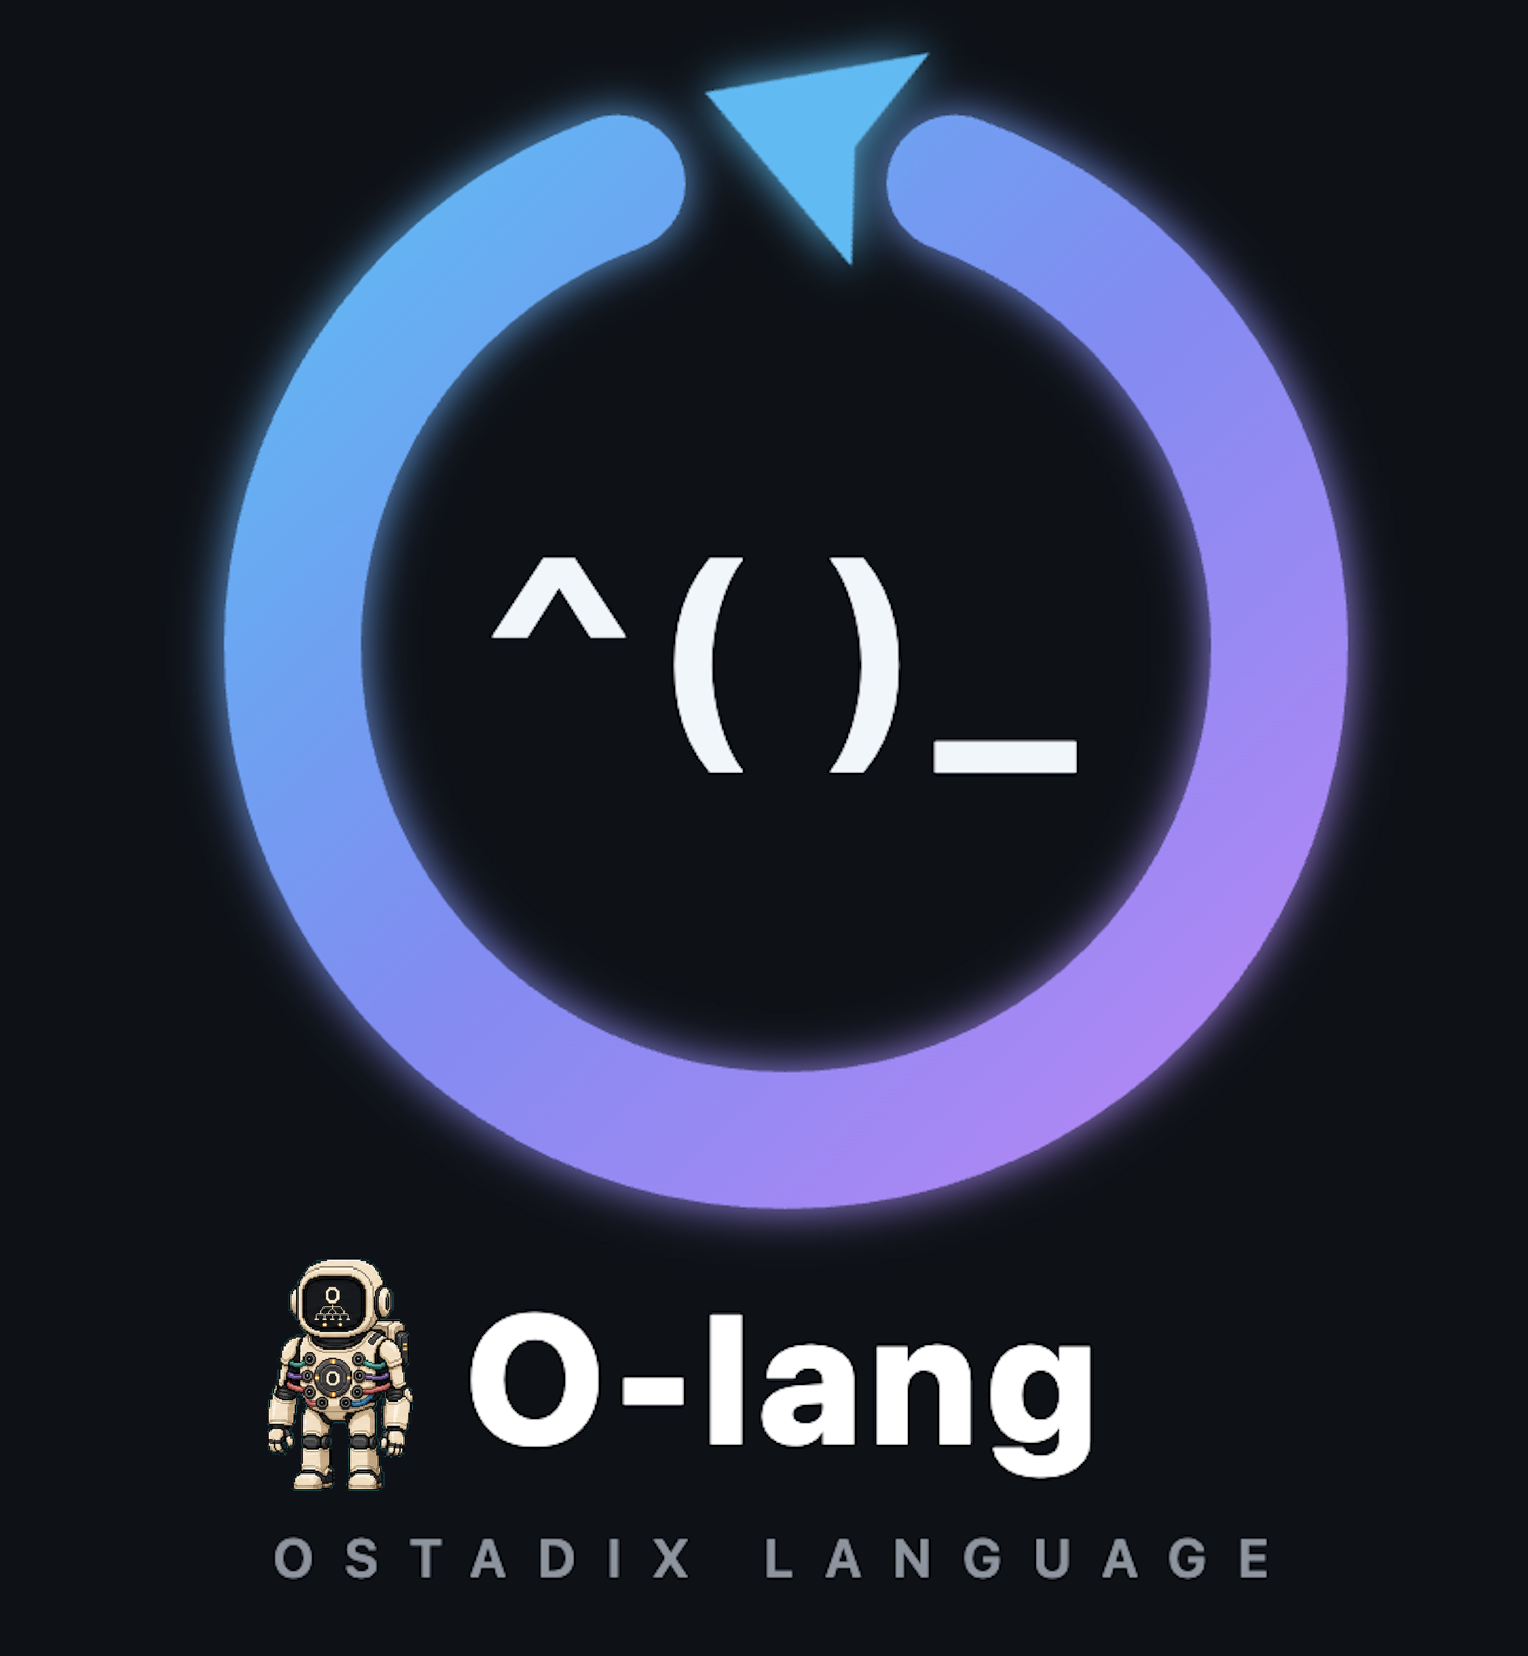
\includegraphics[width=0.46\textwidth]{../assets/olang-logo.png}

  \vspace{0.20in}
  {\fontsize{26}{31}\selectfont\bfseries
  Structural Polyglot Orchestration,\\[0.10in]
  Native O-core, and World Execution\par}

  \vspace{0.16in}
  {\large A technical account of the language, compiler, runtime,\\
  and World architecture\par}

  \vspace{0.24in}
  \begin{tcolorbox}[
    width=0.84\textwidth,colback=ONavy!50!OInk,colframe=OBlue!75,coltext=white,
    boxrule=0.7pt,arc=2pt,left=8pt,right=8pt,top=7pt,bottom=7pt
  ]
  \color{white}\small
  \centering
  \textbf{Implementation snapshot}\\
  \href{https://github.com/lostadi/Ostadix-lang}{github.com/lostadi/Ostadix-lang}\\
  Source snapshot \texttt{36787b16476bc0c8c4ddf665c7228b314d04e716}\\
  Package coordinate \texttt{0.4.0 Unreleased}
  \end{tcolorbox}

  \vspace{0.38in}
  {\large\bfseries Lee Daghlar Ostadi\par}
  \vspace{0.08in}
  {\normalsize ORCID 0009-0001-6380-9558\par}
  \vspace{0.12in}
  {\normalsize 25 August 2026\par}
\end{center}
\end{titlepage}

\color{OInk}
\hypersetup{pageanchor=true}
\pagenumbering{roman}

\section*{Abstract}

I designed \product{} around a direct premise: the evaluator selected for an
expression belongs in the expression's syntax. A hosted source file expresses
that choice through balanced, language-indexed forms such as
\texttt{python\string^(...\string)\_python}. Nested evaluators are structural
nodes, and their results cross language boundaries through \ovalue{}, a typed
interchange algebra. The
authoritative Rust runtime parses these forms into a small structural AST,
lowers every normal execution through \oir{}, freezes backend metadata in a
validated execution plan, projects the plan into a state-complete \hgraph{},
and coordinates backend actors through canonical CBOR. Persistent language
environments, quotation and meta-evaluation, deferred requests, coordination
groups, project lifting, and hosted live-system supervision make evaluator
composition a complete execution model.

I developed \ocore{} as the native systems lineage of this architecture. It is
a statically typed freestanding language whose AST--typed HIR--SSA
MIR--x86-64 assembly/object pipeline supplies code used by the Ostadix kernel.
Its compiler, runtime modules, capability system, and World-admission machinery
carry the architecture from evaluator orchestration into native systems
construction. Together, the hosted and native lineages span polyglot
expression composition, state-complete execution graphs, freestanding
compilation, and authority-bearing World execution.

In this paper I present the complete language system through one exact
implementation snapshot. I explain the hosted grammar and semantics; the
\ovalue{} interchange algebra;
backend actors and authority; \oir{}, execution plans, and \hgraph{}
scheduling; project lifting and route execution; the \ocore{} compiler; and
the Live-World and KernelWorld layers. I then trace the current execution
constitution through Graph V2, Evidence V6, Admission V6, Why V2, the unified
lowercase \texttt{o} front door, reciprocal node pairing, Project Mesh,
Information, Registry V1, and the canonical World formats. The central result
is a coherent architecture in which evaluator identity is syntax,
cross-language state is typed, effects become explicit graph resources, and
execution authority is admitted through exact verified records.

\vspace{0.15in}
\textbf{Keywords:} structural polyglot programming, evaluator composition,
typed interchange values, hypergraph execution, capability systems,
freestanding systems language, multikernel research.

\clearpage
\section*{Core contributions}

\begin{claimbox}[One language system, eight implemented contributions]
\begin{enumerate}
  \item \textbf{Evaluator-indexed syntax.} Every typed expression names its
        evaluator in the grammar, so heterogeneous source remains structurally
        visible in one recursive program tree.
  \item \textbf{Typed inter-language state.} \ovalue{} gives every evaluator a
        common algebra for values, requests, groups, scopes, capabilities, and
        fidelity.
  \item \textbf{State-complete graph execution.} \oir{} and \hgraph{}
        represent values, completion, actor mutation, and world effects as
        explicit dependencies.
  \item \textbf{Whole-project composition.} Deterministic project bundles
        preserve files, routes, guards, artifacts, and alternative policies in
        a reversible language artifact.
  \item \textbf{Native World construction.} \ocore{}, the kernel runtime, and
        KernelWorld carry the same explicit-structure philosophy into
        freestanding compilation and authority-bearing admission.
  \item \textbf{Execution constituted by evidence.} Graph V2 binds the solved
        typed program; Evidence V6 binds its executable environment; Admission
        V6 rederives and materializes the authority consumed by execution.
  \item \textbf{Capacity-first project placement.} Project Mesh moves a
        source-closed project branch with its prerequisites, ranks paired nodes
        by usable capacity, and records generation-fenced attempts.
  \item \textbf{Information and World records.} The Information Kernel,
        eight bounded bridge projections, provenance admission, Registry V1,
        and the OWIDENT, OWPROTO, OWVALUE, and OWRECEIPT codecs give execution
        state canonical identities that can cross implementation boundaries.
\end{enumerate}
\end{claimbox}

\section*{Audience and reading paths}
\addcontentsline{toc}{section}{Audience and reading paths}

I wrote this paper for programming-language researchers, compiler and runtime
engineers, systems and operating-system researchers, and technical readers
evaluating Ostadix-lang as an execution substrate. It assumes familiarity with
abstract syntax trees, intermediate representations, runtime processes, SSA,
capability systems, and virtual-machine execution. Every Ostadix-specific
concept is defined where it first enters the architecture.

The paper develops one continuous argument across three scales. The hosted
language makes evaluator identity part of syntax and carries values between
evaluators through a typed algebra. The compiler turns that structure into an
effect-aware execution graph. \ocore{} and the World layers carry the same
explicit representation discipline into freestanding and authority-bearing
execution.

Every reader can begin with Section~\ref{sec:model}, which presents the whole
system and names its major layers. The paths below then follow each reader's
primary technical question.

\begin{longtable}{P{0.22\textwidth} P{0.41\textwidth} P{0.29\textwidth}}
\toprule
\textbf{Reader} & \textbf{Recommended path} & \textbf{Central question} \\
\midrule
\endhead
Programming-language researcher &
Sections~\ref{sec:syntax}--\ref{sec:ovalue}, Section~\ref{sec:hgraph}, and
Section~\ref{sec:assessment}. &
How does evaluator-indexed syntax become a typed, compositional semantics? \\
Compiler or runtime engineer &
Sections~\ref{sec:constitution}, \ref{sec:ovalue}--\ref{sec:toolchain}, followed by
Section~\ref{sec:validation}. &
How does source become a validated, scheduled, executable graph? \\
Distributed-runtime or agent-tool engineer &
Sections~\ref{sec:constitution}, \ref{sec:projects}, and
\ref{sec:validation}, followed by Section~\ref{sec:boundaries}. &
How do local intent, reciprocal node trust, placement, Information, and World
records preserve one execution identity? \\
Systems or OS researcher &
Sections~\ref{sec:ocore}--\ref{sec:world}, followed by
Sections~\ref{sec:claims} and~\ref{sec:assessment}. &
How does the architecture reach freestanding code, capabilities, and World
admission? \\
Technical adopter or evaluator &
Sections~\ref{sec:syntax}, \ref{sec:projects}, \ref{sec:toolchain}, and
\ref{sec:validation}, followed by the compact reference and reproduction
appendices. &
What can the implementation express, build, inspect, and execute today? \\
\bottomrule
\end{longtable}

\subsection*{How to read the notation, figures, and evidence}

Monospaced text denotes source forms, commands, evaluator identities, resource
names, and emitted compiler labels. \ovalue{}, \oir{}, \hgraph{},
\texttt{HostWorld}, and \texttt{ActorState} name concrete implementation
types or compiler concepts. Architecture figures generally flow from source
on the left toward execution or publication on the right. The complete graph
in Section~\ref{sec:projects} has its own visual grammar and a seven-pass
reading method immediately before the compiler-emitted figure.

Source citations name the implementation file and line interval that realizes
the surrounding mechanism. Validation tables identify the command, observed
result, and validated surface for the implementation release. This lets a
reader move from thesis, to mechanism, to defining code, to executable
evidence without changing terminology.

\tableofcontents
\clearpage
\pagenumbering{arabic}

\section{Implementation basis and method}
\label{sec:scope}

\subsection{Source coordinate}

This paper describes the synchronized Ostadix-lang package coordinate
\texttt{0.4.0 Unreleased} at source snapshot \texttt{36787b16}. The title
page records the complete commit identity. I tie every
technical claim to implementation code, compiler-generated artifacts,
executable tests, or declared evidence gates from this snapshot.

The workspace contains two synchronized Rust packages. The root
\texttt{o-lang} package owns compatibility reexports and command-line
programs. The independently packageable \texttt{ostadix-api} package owns the
parser, IR, evaluator, graph, evidence, scheduler, project, networking,
Information, Registry, World, Live-World, KernelWorld, and O-core runtime
modules. The MCP server is a separately locked Rust package excluded from the
main workspace so its protocol dependencies remain outside the runtime
dependency graph. \src{Cargo.toml}{1--18}
\src{crates/ostadix-api/Cargo.toml}{1--16}
\src{CHANGELOG.md}{8--50}

\subsection{Contribution map}

\begin{longtable}{P{0.20\textwidth} P{0.36\textwidth} P{0.36\textwidth}}
\toprule
\textbf{Contribution} & \textbf{Implementation mechanism} & \textbf{What it enables} \\
\midrule
\endhead
Structural polyglot syntax &
Exact evaluator tags, recursive parser nodes, structural splices, and
persistent actor identities. &
One program tree can contain native Python, SQL, Nix, shell, markup, and other
language regions. \\
Typed exchange &
\ovalue{}, canonical CBOR, renderer contracts, and composed fidelity states. &
Values retain explicit meaning and conversion history while crossing
evaluators. \\
Graph semantics &
\oir{}, validated plans, hyperedges, completion tokens, and versioned resource
states. &
Execution order, effects, mutation, and safe parallelism become inspectable
program structure. \\
Project composition &
Lossless bundles, materialization, route policies, guards, and artifact
collection. &
Whole codebases become reversible, executable Ostadix artifacts. \\
Native World lineage &
\ocore{} HIR/MIR/code generation, kernel capabilities, exact records, and
generation-bound admission. &
The language architecture reaches from hosted composition to machine-level
execution and lifecycle authority. \\
\bottomrule
\end{longtable}

\subsection{Architectural path through the implementation}

The paper follows the implementation from source syntax to execution:

\begin{enumerate}
  \item parse hosted syntax into \texttt{ONode};
  \item lower it to \oir{}, a validated execution plan, and \hgraph{};
  \item trace effects, actor identity, scheduling, process reuse, wire values,
        and authority;
  \item trace project bundling and route execution separately;
  \item trace \ocore{} from lexer through object generation;
  \item trace hosted Live-World, native kernel gates, KernelWorld admission,
        and SVM execution;
  \item rebuild and run the complete applicable gate matrix on the exact snapshot.
\end{enumerate}

\section{The language system in one view}
\label{sec:model}

\product{} is best understood as a family with two compiler lineages and
several execution substrates.

\begin{figure}[htbp]
\centering
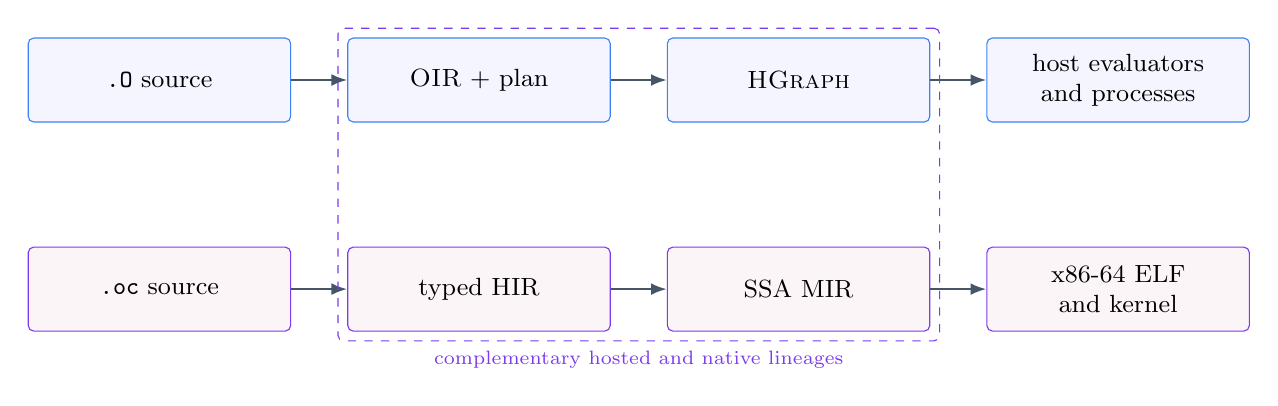
\begin{tikzpicture}[
  node distance=0.31in and 0.28in,
  every node/.style={font=\small},
  box/.style={draw=OLine,rounded corners=2pt,minimum height=0.42in,
    align=center,fill=OLight,text width=1.22in},
  host/.style={box,draw=OBlue,fill=blue!4},
  native/.style={box,draw=OPurple,fill=purple!4},
  arr/.style={-{Latex[length=2mm]},thick,color=OSlate}
]
  \node[host] (osrc) {\texttt{.O} source};
  \node[host,right=of osrc] (oir) {\oir{} + plan};
  \node[host,right=of oir] (hg) {\hgraph{}};
  \node[host,right=of hg] (eval) {host evaluators\\and processes};

  \node[native,below=0.62in of osrc] (ocsrc) {\texttt{.oc} source};
  \node[native,right=of ocsrc] (hir) {typed HIR};
  \node[native,right=of hir] (mir) {SSA MIR};
  \node[native,right=of mir] (elf) {x86-64 ELF\\and kernel};

  \draw[arr] (osrc) -- (oir);
  \draw[arr] (oir) -- (hg);
  \draw[arr] (hg) -- (eval);
  \draw[arr] (ocsrc) -- (hir);
  \draw[arr] (hir) -- (mir);
  \draw[arr] (mir) -- (elf);

  \node[draw=OPurple,dashed,rounded corners=2pt,fit=(oir)(mir),
    label={[font=\scriptsize\color{OPurple}]below:complementary hosted and native lineages}] {};
\end{tikzpicture}
\caption{Compiler bifurcation. Hosted \texttt{.O} orchestrates evaluators;
\texttt{.oc} compiles machine computation.}
\end{figure}

\src{docs/OCORE.md}{3--30}

\subsection{Hosted orchestration}

Hosted O is a compact structural meta-language built from evaluator-indexed
blocks, structural nesting and splicing, bindings, orchestration calls,
persistent evaluator identities, quotation, explicit scopes, and demand
policies. Computation remains native to its selected evaluator while O
supplies the shared program structure.

This design makes Python, SQL, Nix, Markdown, shell, and other runtimes direct
participants in one structurally visible program tree, with each evaluator
retaining its own language semantics.

\subsection{Project execution}

Project execution lifts a directory into a lossless
\texttt{ProjectBundle}. A dedicated subprocess coordinator executes its
routes, dependencies, guards, artifacts, and alternative policies while the
bundle preserves the codebase as one reversible language artifact.

\subsection{Native systems execution}

\ocore{} is a statically typed systems language with modules,
functions, structures, enums, explicit unsafe operations, inline assembly,
and freestanding ABI constraints. Its output can be linked into the Ostadix
kernel. The native lineage gives Ostadix-lang a machine-level
language for implementing the runtime substrate that hosted O can construct,
package, and coordinate.

\subsection{World layers}

Hosted Live-World provides executable local-process lifecycle semantics.
Native kernel modes realize capability-governed services and virtualized
execution. KernelWorld binds exact packages, manifests, policy, architecture,
authority, health, and either package-payload image bytes or the declared
SHA-256 of a user-supplied image into a verified admission chain. These
layers form successive realizations of the World model.

\section{The current execution constitution}
\label{sec:constitution}

The current master makes execution a composed constitutional path. Source
becomes a solved graph. The analyzer binds that graph to runtime facts. The
admission compiler reproduces those facts and materializes the inputs that the
coordinator consumes. Local commands, agent tools, and Project Mesh all enter
that path through explicit records. Information and World formats preserve the
identities needed to inspect, move, and verify the resulting computation.

\subsection{Independent \texttt{ostadix-api} ownership}

I separated implementation ownership from command-line packaging. The
publishable \texttt{ostadix-api} crate owns the runtime engine and its nominal
types. The root \texttt{o-lang} package depends on the exact synchronized
engine version and reexports the engine modules used by established
\texttt{o\_lang::} callers. A value parsed through the root library and a value
handled through \texttt{ostadix\_api} therefore have one defining type and one
runtime implementation.

\begin{figure}[htbp]
\centering
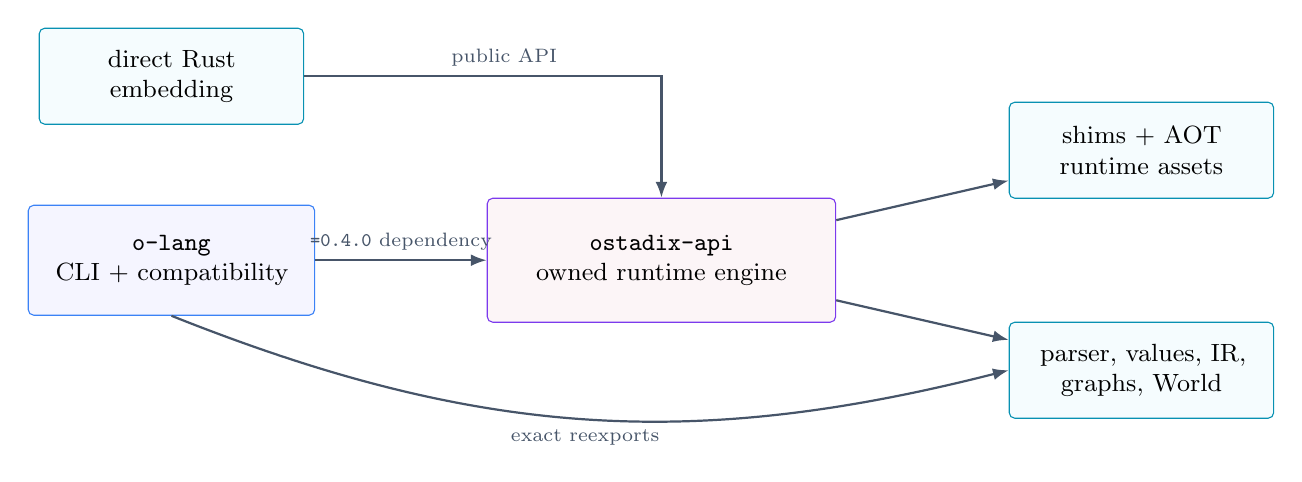
\begin{tikzpicture}[
  x=1in,y=1in,
  every node/.style={font=\small},
  shell/.style={draw=OBlue,rounded corners=2pt,fill=blue!4,
    text width=1.34in,minimum height=0.55in,align=center},
  engine/.style={draw=OPurple,rounded corners=2pt,fill=purple!4,
    text width=1.65in,minimum height=0.62in,align=center},
  client/.style={draw=OCyan,rounded corners=2pt,fill=cyan!4,
    text width=1.23in,minimum height=0.48in,align=center},
  arr/.style={-{Latex[length=2mm]},thick,color=OSlate}
]
  \node[shell] (root) at (0,0) {\texttt{o-lang}\\CLI + compatibility};
  \node[client] (embed) at (0,0.92) {direct Rust\\embedding};
  \node[engine] (api) at (2.45,0) {\texttt{ostadix-api}\\owned runtime engine};
  \node[client] (assets) at (4.85,0.55) {shims + AOT\\runtime assets};
  \node[client] (types) at (4.85,-0.55) {parser, values, IR,\\graphs, World};
  \draw[arr] (embed.east) -| node[pos=0.28,above,font=\scriptsize]
    {public API} (api.north);
  \draw[arr] (root) -- node[above,font=\scriptsize]
    {\texttt{=0.4.0} dependency} (api);
  \draw[arr] (root.south) to[bend right=18]
    node[below,font=\scriptsize] {exact reexports} (types.west);
  \draw[arr] (api) -- (assets);
  \draw[arr] (api) -- (types);
\end{tikzpicture}
\caption{One engine owns runtime behavior. The root package supplies commands
and preserves established imports by reexporting the engine's exact types.}
\label{fig:api-ownership}
\end{figure}

The ownership boundary is enforced by the workspace and package manifests,
the engine module root, and the root's one-way reexport list.
\src{Cargo.toml}{14--18}
\src{Cargo.toml}{82--86}
\src{crates/ostadix-api/Cargo.toml}{1--16}
\src{crates/ostadix-api/src/lib.rs}{1--59}
\src{src/lib.rs}{1--13}

\subsection{The unified lowercase \texttt{o} front door}

The lowercase \texttt{o} command is the language's intent front door. Its
compiled path implements \texttt{run}, \texttt{plan}, \texttt{explain}, and
\texttt{inspect}; the repository dispatcher routes those verbs into
\texttt{o-cli} and retains the remaining operational command families. The
front door classifies an input as hosted O source, a directory, a lifted
project, or an accepted standalone form, then selects the ordinary evaluator
or project engine and renders one stable intent record.

\begin{lstlisting}[style=plaincode]
o run program.O
o plan program.O
o explain last-run
o inspect last-run

o run ./project --route main
o plan ./project --route main
\end{lstlisting}

Each completed run yields a durable \texttt{RunRecordV1}. The record binds a
schema, run identity, wall-clock time, resolved intent, engine selection,
source identity, execution result, and optional trace attachment. The store
uses canonical JSON bytes, validates every record before acceptance, writes
through a temporary file, renames atomically, and maintains the selected
history root. Record identity is content-bound, so inspection names the
artifact that was actually persisted.

\begin{figure}[htbp]
\centering
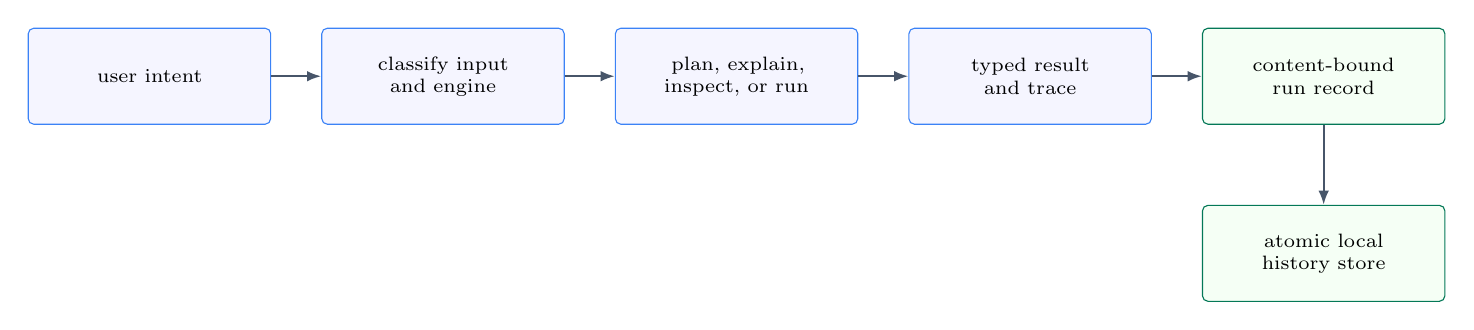
\begin{tikzpicture}[
  node distance=0.25in,
  n/.style={draw=OBlue,rounded corners=2pt,fill=blue!4,
    text width=1.12in,minimum height=0.48in,align=center,font=\scriptsize},
  r/.style={draw=OGreen,rounded corners=2pt,fill=green!4,
    text width=1.12in,minimum height=0.48in,align=center,font=\scriptsize},
  a/.style={-{Latex[length=1.8mm]},thick,color=OSlate}
]
  \node[n] (argv) {user intent};
  \node[n,right=of argv] (classify) {classify input\\and engine};
  \node[n,right=of classify] (act) {plan, explain,\\inspect, or run};
  \node[n,right=of act] (result) {typed result\\and trace};
  \node[r,right=of result] (record) {content-bound\\run record};
  \node[r,below=0.40in of record] (store) {atomic local\\history store};
  \foreach \x/\y in {argv/classify,classify/act,act/result,result/record}
    {\draw[a] (\x) -- (\y);}
  \draw[a] (record) -- (store);
\end{tikzpicture}
\caption{The lowercase front door converts command intent into a resolved
execution path and a durable record that can be inspected later.}
\label{fig:o-front-door}
\end{figure}

\src{scripts/o-cli.sh}{18--26}
\src{src/bin/o-cli.rs}{42--68}
\src{src/bin/o-cli.rs}{403--410}
\src{src/bin/o-cli.rs}{472--517}
\src{src/bin/o-cli.rs}{931--990}
\src{src/bin/o-cli.rs}{992--1066}
\src{src/bin/o-cli.rs}{1641--1676}
\src{crates/ostadix-api/src/intent/record.rs}{25--29}
\src{crates/ostadix-api/src/intent/record.rs}{53--100}
\src{crates/ostadix-api/src/intent/record.rs}{894--955}
\src{crates/ostadix-api/src/intent/store.rs}{1--6}
\src{crates/ostadix-api/src/intent/store.rs}{27--35}
\src{crates/ostadix-api/src/intent/store.rs}{84--144}

\subsection{Graph V2, Evidence V6, Admission V6, and Why V2}
\label{sec:v6}

Graph V2 is the executable identity of a solved hosted program. Its canonical
digest covers graph nodes, typed values, actor identities, the complete typed
fidelity assessment, executable operations, effects, sequence dependencies,
roots, and bindings. A semantic change in any of those fields produces a
different graph coordinate.

Evidence V6 binds that graph to the complete lowering and execution context.
The bundle carries the OIR and plan identities, Graph V2 identity, analyzer
coordinate, backend Catalog V5 projection, backend artifact bindings, runtime
binding, environment binding, ambient World binding, and one typed assessment
for every executable operation. The analyzer first validates the caller graph
against a freshly solved Graph V2 before emitting the bundle.

Admission V6 is the executable authority compiler. It checks the schema and
analyzer coordinate, re-solves and re-analyzes the graph, matches the complete
operation inventory, verifies every hard assessment, materializes admission
evidence nodes, validates the admitted graph, and constructs its ready
schedule. The coordinator and evaluator accept the resulting
\texttt{AdmittedExecution} object.

Why V2 is the reader-facing explanation of that authority. For a selected plan
node it reports the admitted operation, its inputs and outputs, effect and
actor rails, dependency witnesses, typed fidelity decision, and schedule
position. It is derived from Admission V6 as an inspection operation.

\begin{figure}[htbp]
\centering
\resizebox{\linewidth}{!}{%
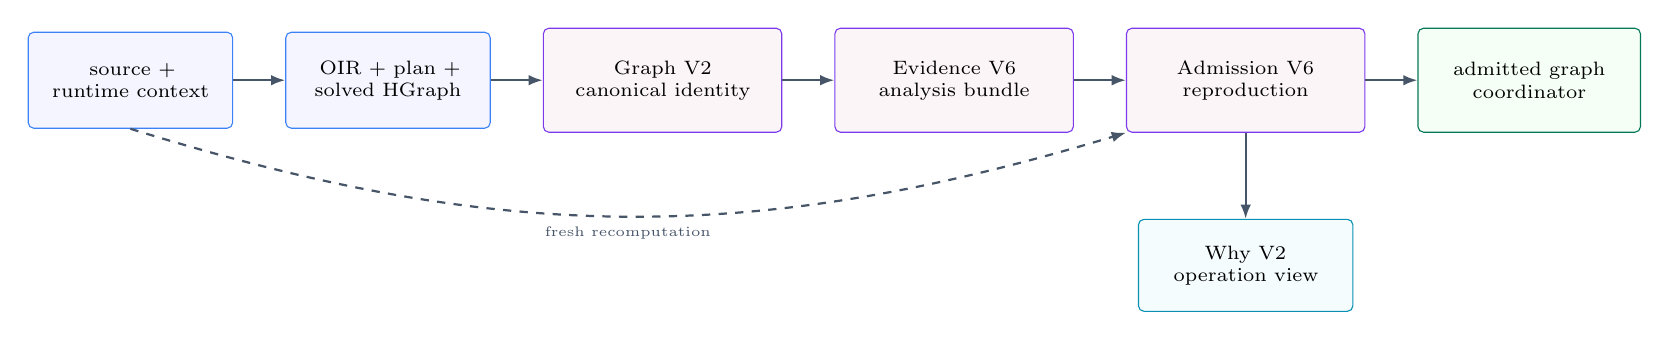
\begin{tikzpicture}[
  node distance=0.26in,
  every node/.style={font=\scriptsize},
  source/.style={draw=OBlue,rounded corners=2pt,fill=blue!4,
    text width=0.93in,minimum height=0.48in,align=center},
  proof/.style={draw=OPurple,rounded corners=2pt,fill=purple!4,
    text width=1.10in,minimum height=0.52in,align=center},
  exec/.style={draw=OGreen,rounded corners=2pt,fill=green!4,
    text width=1.02in,minimum height=0.52in,align=center},
  view/.style={draw=OCyan,rounded corners=2pt,fill=cyan!4,
    text width=0.98in,minimum height=0.46in,align=center},
  arr/.style={-{Latex[length=1.8mm]},thick,color=OSlate}
]
  \node[source] (src) {source +\\runtime context};
  \node[source,right=of src] (lower) {OIR + plan +\\solved HGraph};
  \node[proof,right=of lower] (graph) {Graph V2\\canonical identity};
  \node[proof,right=of graph] (evidence) {Evidence V6\\analysis bundle};
  \node[proof,right=of evidence] (admit) {Admission V6\\reproduction};
  \node[exec,right=of admit] (run) {admitted graph\\coordinator};
  \node[view,below=0.43in of admit] (why) {Why V2\\operation view};
  \foreach \x/\y in {src/lower,lower/graph,graph/evidence,evidence/admit,admit/run}
    {\draw[arr] (\x) -- (\y);}
  \draw[arr] (admit) -- (why);
  \draw[arr,dashed] (src.south) to[bend right=17]
    node[below,font=\tiny] {fresh recomputation} (admit.south west);
\end{tikzpicture}
}
\caption{Current hosted execution is a proof-producing and proof-consuming
pipeline. Admission reproduces the analyzer result before execution begins.}
\label{fig:v6-pipeline}
\end{figure}

\begin{longtable}{P{0.17\textwidth} P{0.30\textwidth} P{0.45\textwidth}}
\toprule
\textbf{Coordinate} & \textbf{Primary object} & \textbf{Mechanism} \\
\midrule
\endhead
Graph V2 & Solved executable \hgraph{} & Canonical identity over executable
shape, typed values, effects, actor state, fidelity, roots, and bindings. \\
Evidence V6 & \texttt{EvidenceBundleV6} & Analyzer result bound to graph,
lowering, catalog, artifacts, runtime, environment, and World. \\
Admission V6 & \texttt{AdmittedExecution} & Fresh reproduction, complete
per-operation validation, evidence materialization, and ready scheduling. \\
Why V2 & \texttt{ScheduleWhyV2} & Stable operation neighborhood projected
from the admitted schedule for human and tool inspection. \\
\bottomrule
\end{longtable}

\src{crates/ostadix-api/src/evidence/fact.rs}{10--15}
\src{crates/ostadix-api/src/evidence/fact.rs}{460--493}
\src{crates/ostadix-api/src/evidence/analyze.rs}{33--36}
\src{crates/ostadix-api/src/evidence/analyze.rs}{239--272}
\src{crates/ostadix-api/src/evidence/analyze.rs}{624--676}
\src{crates/ostadix-api/src/evidence/analyze.rs}{702--769}
\src{crates/ostadix-api/src/evidence/analyze.rs}{792--809}
\src{crates/ostadix-api/src/evidence/analyze.rs}{818--953}
\src{crates/ostadix-api/src/evidence/admit.rs}{105--114}
\src{crates/ostadix-api/src/evidence/admit.rs}{195--231}
\src{crates/ostadix-api/src/evidence/admit.rs}{274--330}
\src{crates/ostadix-api/src/evidence/admit.rs}{1882--1989}
\src{crates/ostadix-api/src/evidence/admit.rs}{2201--2335}
\src{src/bin/olangc.rs}{1332--1372}

\subsection{The ten-tool Ostadix MCP}
\label{sec:mcp}

The Ostadix MCP is part of this master snapshot. It is a standalone
Rust/\texttt{rmcp} stdio server with its own lockfile, built by default through
\texttt{setup.sh} and registered by the repository's \path{.mcp.json}. Its ten
tools expose environment, runtime, Information, compilation, execution, and
diagnostic operations through resolved repository and command-line contracts.

\begin{longtable}{P{0.25\textwidth} P{0.67\textwidth}}
\toprule
\textbf{Tool} & \textbf{Owned operation} \\
\midrule
\endhead
\texttt{o\_env} & Report the resolved repository, backend, binary, and runtime
environment used by subsequent tools. \\
\texttt{o\_runtimes} & Enumerate every canonical evaluator backend and report
its executable requirements and current local availability. \\
\texttt{o\_information\_inspect} & Read the current Information root through
the bounded existing-root inspection path. \\
\texttt{o\_smoke} & Execute the canonical hosted smoke program and report its
result. \\
\texttt{o\_run} & Run a hosted input through the direct evaluator path. \\
\texttt{o\_analyze\_intent} & Resolve an intent, compute current analysis,
and return a bounded execution handle. \\
\texttt{o\_execute\_intent} & Consume one analysis handle and ask the root O
process to reproduce and admit the execution. \\
\texttt{o\_olangc} & Invoke the compiler's IR, DOT, script, binary, or WASM
surface with checked arguments. \\
\texttt{o\_doctor} & Diagnose repository, backends, binaries, and runtime
availability. \\
\texttt{o\_search\_run} & Run a named a18re search tool from an explicitly
selected work directory, \texttt{A18\_WORK}, or the local a18re default, using
the resolved O executable and backend directory. \\
\bottomrule
\end{longtable}

Analyze then execute forms a one-use authorization protocol. The server binds
the handle to program bytes, working directory, repository root, backend
directory, source identity, and resolved intent. It gives the entry a bounded
lifetime and removes it before execution validation. The root O process
receives the bound request, recomputes current Graph V2 and Evidence V6, and
constructs fresh Admission V6 authority. A successful response therefore
connects the agent-visible intent to the same current execution constitution
used by the language runtime.

\begin{figure}[htbp]
\centering
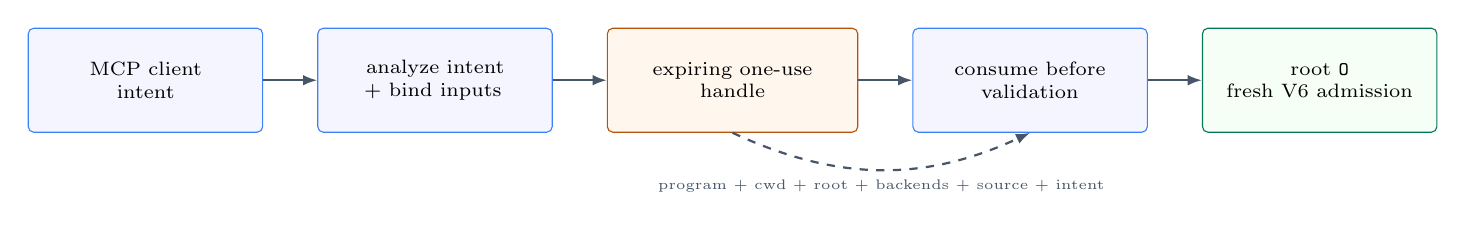
\begin{tikzpicture}[
  node distance=0.27in,
  n/.style={draw=OBlue,rounded corners=2pt,fill=blue!4,
    text width=1.08in,minimum height=0.52in,align=center,font=\scriptsize},
  token/.style={draw=OAmber,rounded corners=2pt,fill=orange!7,
    text width=1.16in,minimum height=0.52in,align=center,font=\scriptsize},
  e/.style={draw=OGreen,rounded corners=2pt,fill=green!4,
    text width=1.08in,minimum height=0.52in,align=center,font=\scriptsize},
  a/.style={-{Latex[length=1.8mm]},thick,color=OSlate}
]
  \node[n] (client) {MCP client\\intent};
  \node[n,right=of client] (analyze) {analyze intent\\+ bind inputs};
  \node[token,right=of analyze] (handle) {expiring one-use\\handle};
  \node[n,right=of handle] (consume) {consume before\\validation};
  \node[e,right=of consume] (root) {root \texttt{O}\\fresh V6 admission};
  \foreach \x/\y in {client/analyze,analyze/handle,handle/consume,consume/root}
    {\draw[a] (\x) -- (\y);}
  \draw[a,dashed] (handle.south) to[bend right=25]
    node[below,font=\tiny] {program + cwd + root + backends + source + intent}
    (consume.south);
\end{tikzpicture}
\caption{The MCP analyze/execute protocol carries a bounded intent binding
into a fresh root-runtime admission.}
\label{fig:mcp-handle}
\end{figure}

\src{mcp/ostadix_lang_mcp_server/Cargo.toml}{1--12}
\src{mcp/ostadix_lang_mcp_server/Cargo.toml}{26--32}
\src{setup.sh}{886--910}
\src{setup.sh}{1582--1586}
\src{.mcp.json}{1--7}
\src{mcp/ostadix_lang_mcp_server/src/main.rs}{43--68}
\src{mcp/ostadix_lang_mcp_server/src/main.rs}{77--187}
\src{mcp/ostadix_lang_mcp_server/src/main.rs}{1663--1766}
\src{mcp/ostadix_lang_mcp_server/src/main.rs}{1768--1864}
\src{mcp/ostadix_lang_mcp_server/src/main.rs}{1858--2015}
\src{mcp/ostadix_lang_mcp_server/src/main.rs}{2018--2207}
\src{mcp/ostadix_lang_mcp_server/src/main.rs}{2209--2222}
\src{src/main.rs}{81--128}
\src{src/main.rs}{161--225}
\src{crates/ostadix-api/src/eval.rs}{2455--2506}

\subsection{Reciprocal LAN pairing and pinned TLS}
\label{sec:pairing}

Node trust begins with a reciprocal, one-use, ten-digit pairing code. Each node
creates an ephemeral SPAKE2 role and validates the peer transcript. Directional
HKDF and HMAC keys bind the code, both node identities, both endpoints, both
nonces, and the full request/response transcript. Each destination then issues
the client certificate it will accept for the peer. Private keys remain local;
the stored peer record carries the destination CA, destination server name,
client certificate, and generation needed for the next TLS session.

The data plane uses TLS 1.3 with the Ostadix ALPN token. Outbound connection
validation loads the paired destination CA and checks the stored server name.
The node listener validates client certificates against its pairing CA before
the application protocol receives a request. Discovery supplies addresses;
the paired record supplies identity and cryptographic continuity.

\begin{figure}[htbp]
\centering
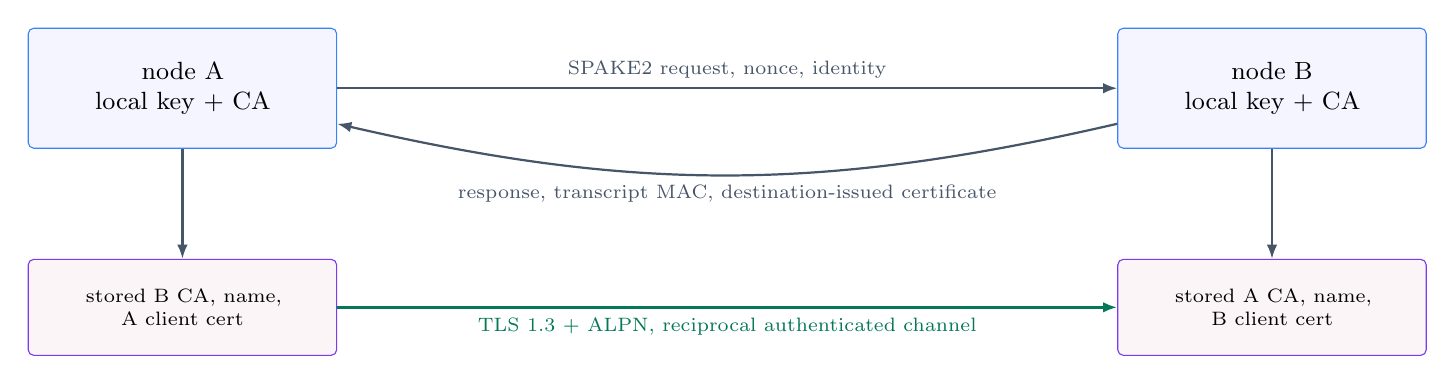
\begin{tikzpicture}[
  node distance=0.30in and 0.68in,
  host/.style={draw=OBlue,rounded corners=2pt,fill=blue!4,
    text width=1.45in,minimum height=0.60in,align=center,font=\small},
  fact/.style={draw=OPurple,rounded corners=2pt,fill=purple!4,
    text width=1.45in,minimum height=0.48in,align=center,font=\scriptsize},
  a/.style={-{Latex[length=1.8mm]},thick,color=OSlate}
]
  \node[host] (a) {node A\\local key + CA};
  \node[host,right=3.9in of a] (b) {node B\\local key + CA};
  \node[fact,below=0.55in of a] (ap) {stored B CA, name,\\A client cert};
  \node[fact,below=0.55in of b] (bp) {stored A CA, name,\\B client cert};
  \draw[a] (a) -- node[above,font=\scriptsize] {SPAKE2 request, nonce,
    identity} (b);
  \draw[a] (b) to[bend left=13] node[below,font=\scriptsize] {response,
    transcript MAC, destination-issued certificate} (a);
  \draw[a] (a) -- (ap);
  \draw[a] (b) -- (bp);
  \draw[a,very thick,OGreen] (ap) -- node[below,font=\scriptsize]
    {TLS 1.3 + ALPN, reciprocal authenticated channel} (bp);
\end{tikzpicture}
\caption{Pairing turns a short shared code into reciprocal destination pins and
client credentials. Those persisted facts establish later node channels.}
\label{fig:pairing}
\end{figure}

\src{crates/ostadix-api/src/hosted_remote/pairing.rs}{1--7}
\src{crates/ostadix-api/src/hosted_remote/pairing.rs}{24--76}
\src{crates/ostadix-api/src/hosted_remote/pairing.rs}{79--193}
\src{crates/ostadix-api/src/hosted_remote/pairing.rs}{195--387}
\src{crates/ostadix-api/src/hosted_remote/pairing.rs}{389--586}
\src{crates/ostadix-api/src/hosted_remote/pairing.rs}{684--815}
\src{crates/ostadix-api/src/hosted_remote/lan.rs}{693--870}
\src{src/bin/o-node.rs}{1070--1175}
\src{src/bin/octl.rs}{874--970}
\src{crates/ostadix-api/src/hosted_remote/tls.rs}{61--156}
\src{crates/ostadix-api/src/hosted_remote/tls.rs}{204--303}

\subsection{Capacity-first Project Mesh}
\label{sec:mesh}

Project Mesh distributes a project at the route-branch scale. The planner
selects the requested route branch and closes it over prerequisite routes,
inputs, declared artifacts, and bundle provenance. Candidate nodes come from
paired authenticated discovery and carry current profile, compatibility, and
capacity facts. Ranking places usable execution capacity first, then applies
the route and policy constraints that preserve semantic compatibility.

The selected node receives a source-closed project payload and a bounded
execution request. Generation fences bind discovery, reservation, attempt,
and result state. Retry contracts record why an attempt can continue, while
concurrent selection policies record all relevant attempts and their terminal
settlement. Mesh traces therefore connect placement decisions to the exact
project branch, node generation, and returned artifacts.

\begin{figure}[htbp]
\centering
\resizebox{\linewidth}{!}{%
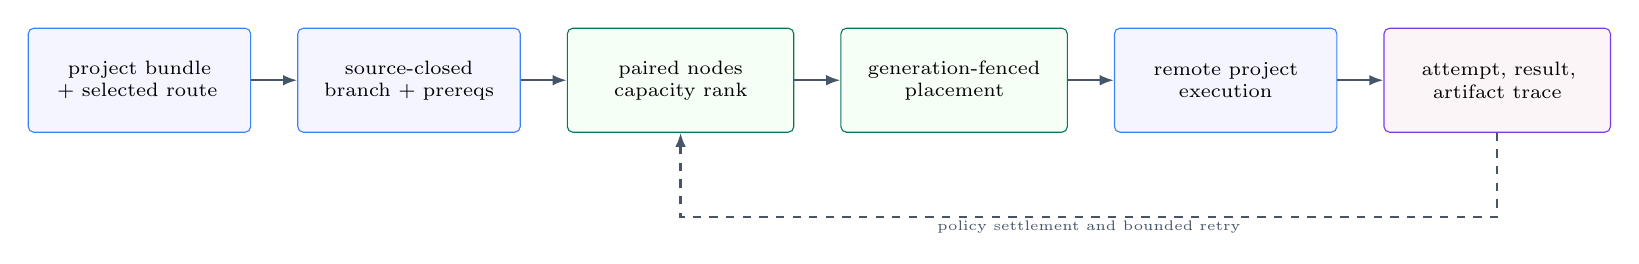
\begin{tikzpicture}[
  node distance=0.23in,
  n/.style={draw=OBlue,rounded corners=2pt,fill=blue!4,
    text width=1.02in,minimum height=0.52in,align=center,font=\scriptsize},
  c/.style={draw=OGreen,rounded corners=2pt,fill=green!4,
    text width=1.04in,minimum height=0.52in,align=center,font=\scriptsize},
  t/.style={draw=OPurple,rounded corners=2pt,fill=purple!4,
    text width=1.04in,minimum height=0.52in,align=center,font=\scriptsize},
  a/.style={-{Latex[length=1.8mm]},thick,color=OSlate}
]
  \node[n] (project) {project bundle\\+ selected route};
  \node[n,right=of project] (closure) {source-closed\\branch + prereqs};
  \node[c,right=of closure] (rank) {paired nodes\\capacity rank};
  \node[c,right=of rank] (place) {generation-fenced\\placement};
  \node[n,right=of place] (execute) {remote project\\execution};
  \node[t,right=of execute] (trace) {attempt, result,\\artifact trace};
  \foreach \x/\y in {project/closure,closure/rank,rank/place,place/execute,execute/trace}
    {\draw[a] (\x) -- (\y);}
  \coordinate (retryR) at ([yshift=-0.42in]trace.south);
  \coordinate (retryL) at ([yshift=-0.42in]rank.south);
  \draw[a,dashed] (trace.south) -- (retryR) --
    node[below,font=\tiny,fill=white,inner sep=1pt]
      {policy settlement and bounded retry}
    (retryL) -- (rank.south);
\end{tikzpicture}
}
\caption{Project Mesh moves a complete route branch, chooses capacity, binds
node generations, and returns a causally connected attempt trace.}
\label{fig:project-mesh}
\end{figure}

\src{crates/ostadix-api/src/hosted_remote/project_mesh.rs}{1--6}
\src{crates/ostadix-api/src/hosted_remote/project_mesh.rs}{45--112}
\src{crates/ostadix-api/src/hosted_remote/project_mesh.rs}{278--375}
\src{crates/ostadix-api/src/hosted_remote/project_mesh.rs}{804--895}
\src{crates/ostadix-api/src/hosted_remote/project_mesh.rs}{1024--1117}
\src{crates/ostadix-api/src/hosted_remote/project_mesh.rs}{1810--2018}
\src{crates/ostadix-api/src/hosted_remote/project_mesh.rs}{2092--2243}
\src{crates/ostadix-api/src/hosted_remote/project_mesh.rs}{2260--2335}
\src{crates/ostadix-api/src/hosted_remote/mesh.rs}{1510--1719}

\subsection{Information Kernel, Bridge, and Provenance}
\label{sec:information}

The Information Kernel turns observations into content-addressed information
state. An entity descriptor identifies what a fact is about. An Information
Atom binds that entity, a typed payload tier, assertions, and provenance.
Snapshots assemble atom identities into one immutable view. Revisions advance
named roots through compare-and-swap, so a reader can identify the exact view
it observed and a writer can prove the predecessor it replaced.

Payload tiers keep size and meaning explicit. T0 carries bounded public
scalars. T1 identifies content held by the managed blob store. T2 identifies
external content through canonical schema, media type, digest, and logical
length. Canonical CBOR and domain-separated SHA-256 give every atom, blob,
snapshot, and revision a stable identity.

Information Bridge V1 defines exactly eight bounded projections:

\begin{enumerate}
  \item parsed document identity and structural counts;
  \item allowlisted public scalar value identity;
  \item solved HGraph metadata;
  \item exact Evidence V6 metadata;
  \item verified Registry V1 profile metadata;
  \item verified World receipt identity and semantic digest;
  \item logical project graph identity; and
  \item Hosted V2 journal-entry identity.
\end{enumerate}

Each projection has a private wire shape, strict schema check, bounded
canonical-CBOR decoder, and canonical re-encode check. The bridge chooses the
metadata that belongs in Information and hashes identifiers whose native
locator vocabulary should remain outside the Information record.

Information Provenance V2 adds a content-addressed sidecar over frozen atom
identities. Typed witnesses describe acquisition, producer authentication,
procedure, signer authorization, receipt currentness, plan-node attribution,
execution and effect fidelity, and morphism fidelity. Admission recomputes the
sidecar image, verifies the bound World receipt and execution evidence, then
derives a recovery assessment with intrinsic loss, discharged obligations,
and unresolved obligations. Exact recovery establishes an origin statement
that can be presented to Information readers.

\begin{figure}[htbp]
\centering
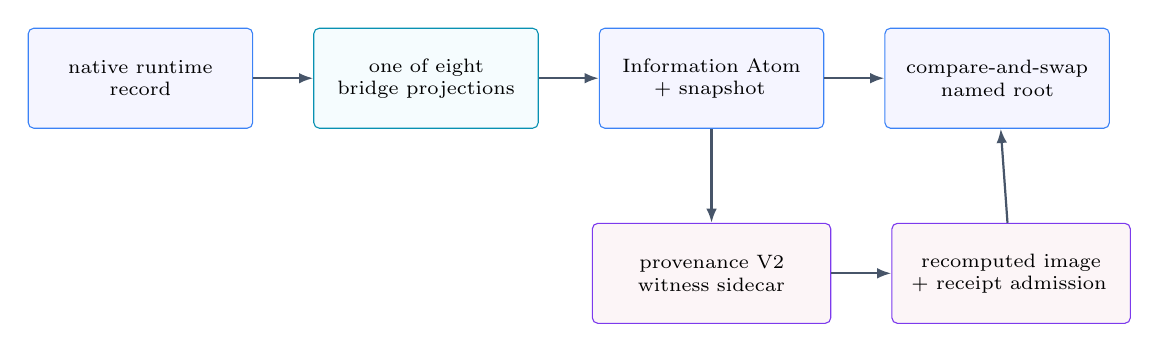
\begin{tikzpicture}[
  node distance=0.23in and 0.30in,
  every node/.style={font=\scriptsize},
  k/.style={draw=OBlue,rounded corners=2pt,fill=blue!4,
    text width=1.03in,minimum height=0.50in,align=center},
  b/.style={draw=OCyan,rounded corners=2pt,fill=cyan!4,
    text width=1.03in,minimum height=0.50in,align=center},
  p/.style={draw=OPurple,rounded corners=2pt,fill=purple!4,
    text width=1.10in,minimum height=0.50in,align=center},
  a/.style={-{Latex[length=1.8mm]},thick,color=OSlate}
]
  \node[k] (native) {native runtime\\record};
  \node[b,right=of native] (project) {one of eight\\bridge projections};
  \node[k,right=of project] (atom) {Information Atom\\+ snapshot};
  \node[k,right=of atom] (root) {compare-and-swap\\named root};
  \node[p,below=0.47in of atom] (sidecar) {provenance V2\\witness sidecar};
  \node[p,right=of sidecar] (admit) {recomputed image\\+ receipt admission};
  \foreach \x/\y in {native/project,project/atom,atom/root,sidecar/admit}
    {\draw[a] (\x) -- (\y);}
  \draw[a] (atom) -- (sidecar);
  \draw[a] (admit) -- (root);
\end{tikzpicture}
\caption{Native facts enter the Information Kernel through explicit bounded
projections; provenance sidecars add typed recovery evidence to frozen atom
identity.}
\label{fig:information-path}
\end{figure}

\src{crates/ostadix-api/src/information/mod.rs}{1--7}
\src{crates/ostadix-api/src/information/mod.rs}{22--60}
\src{crates/ostadix-api/src/information/model.rs}{20--38}
\src{crates/ostadix-api/src/information/model.rs}{143--245}
\src{crates/ostadix-api/src/information/model.rs}{275--298}
\src{crates/ostadix-api/src/information/model.rs}{354--410}
\src{crates/ostadix-api/src/information/model.rs}{448--500}
\src{crates/ostadix-api/src/information/root.rs}{5--123}
\src{crates/ostadix-api/src/information/provenance.rs}{1--8}
\src{crates/ostadix-api/src/information/provenance.rs}{119--213}
\src{crates/ostadix-api/src/information/provenance.rs}{424--475}
\src{crates/ostadix-api/src/information/provenance.rs}{721--810}
\src{crates/ostadix-api/src/information_bridge/mod.rs}{1--6}
\src{crates/ostadix-api/src/information_bridge/mod.rs}{25--54}
\src{crates/ostadix-api/src/information_bridge/mod.rs}{74--164}
\src{crates/ostadix-api/src/information_bridge/mod.rs}{283--317}
\src{crates/ostadix-api/src/information_bridge/mod.rs}{527--601}
\src{crates/ostadix-api/src/information_bridge/mod.rs}{871--1037}
\src{crates/ostadix-api/src/information_provenance/mod.rs}{1--7}
\src{crates/ostadix-api/src/information_provenance/mod.rs}{28--38}
\src{crates/ostadix-api/src/information_provenance/mod.rs}{74--194}
\src{crates/ostadix-api/src/information_provenance/mod.rs}{330--505}

\subsection{Registry V1}
\label{sec:registry}

Registry V1 is an append-only Ed25519 namespace and node-profile chain. A
namespace root establishes the trust anchor and validity interval. A root or
delegate can authorize a strict descendant namespace. Profile publications
bind a namespace, node identity, generation-bearing node profile, issue time,
and expiry. Every event carries its sequence, predecessor digest, namespace,
signer key, and signed body.

Verification walks the chain from configured anchors, validates signatures and
delegation scope, enforces time bounds and profile freshness, and maintains the
highest accepted generation for each node. Sequence, predecessor, rollback,
and equivocation checks turn a local event file into a verifiable publication
history. The resulting \texttt{VerifiedRegistryProfileV1} is the profile form
consumed by placement and Information projection.

\begin{figure}[htbp]
\centering
\resizebox{\linewidth}{!}{%
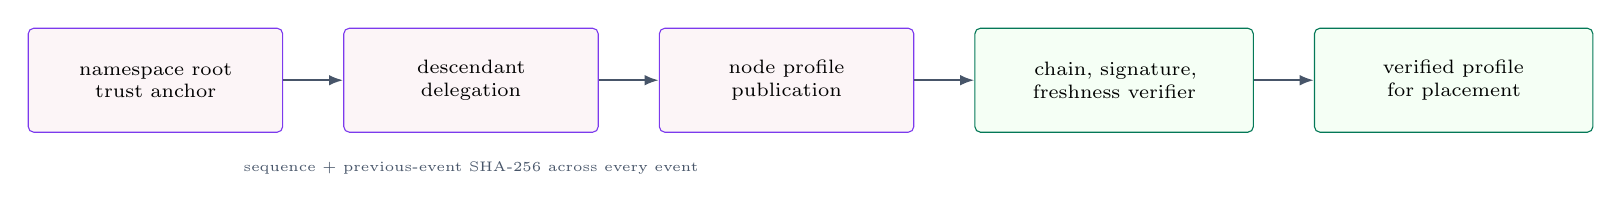
\begin{tikzpicture}[
  node distance=0.30in,
  e/.style={draw=OPurple,rounded corners=2pt,fill=purple!4,
    text width=1.18in,minimum height=0.52in,align=center,font=\scriptsize},
  v/.style={draw=OGreen,rounded corners=2pt,fill=green!4,
    text width=1.30in,minimum height=0.52in,align=center,font=\scriptsize},
  a/.style={-{Latex[length=1.8mm]},thick,color=OSlate}
]
  \node[e] (root) {namespace root\\trust anchor};
  \node[e,right=of root] (delegation) {descendant\\delegation};
  \node[e,right=of delegation] (profile) {node profile\\publication};
  \node[v,right=of profile] (verify) {chain, signature,\\freshness verifier};
  \node[v,right=of verify] (owned) {verified profile\\for placement};
  \foreach \x/\y in {root/delegation,delegation/profile,profile/verify,verify/owned}
    {\draw[a] (\x) -- (\y);}
  \node[font=\tiny\color{OSlate},below=0.10in of delegation]
    {sequence + previous-event SHA-256 across every event};
\end{tikzpicture}
}
\caption{Registry V1 turns signed namespace events into a freshness-checked
node profile suitable for placement decisions.}
\label{fig:registry}
\end{figure}

\src{crates/ostadix-api/src/registry/mod.rs}{1--5}
\src{crates/ostadix-api/src/registry/mod.rs}{18--67}
\src{crates/ostadix-api/src/registry/model.rs}{9--22}
\src{crates/ostadix-api/src/registry/model.rs}{24--74}
\src{crates/ostadix-api/src/registry/model.rs}{76--152}
\src{crates/ostadix-api/src/registry/model.rs}{154--245}
\src{crates/ostadix-api/src/registry/model.rs}{299--340}
\src{crates/ostadix-api/src/registry/crypto.rs}{14--60}
\src{crates/ostadix-api/src/registry/crypto.rs}{70--225}
\src{crates/ostadix-api/src/registry/verify.rs}{55--226}
\src{crates/ostadix-api/src/registry/verify.rs}{227--348}
\src{crates/ostadix-api/src/registry/verify.rs}{393--442}

\subsection{World identities, values, protocols, and receipts}
\label{sec:world-codecs}

The World layer uses four separate canonical formats. Separation keeps each
decoder's vocabulary, size ceiling, and authority meaning explicit.

\begin{longtable}{P{0.17\textwidth} P{0.20\textwidth} P{0.47\textwidth}}
\toprule
\textbf{Format} & \textbf{Primary unit} & \textbf{Mechanism} \\
\midrule
\endhead
\texttt{OWIDENT V1} & World identity atom & Deterministic identity-only
records with strict nonzero generation, term, version, and index rules plus
hierarchical stale and logical comparison. \\
\texttt{OWPROTO V1} & Bounded protocol record & Big-endian framing, four fixed
record kinds, exact-length and reserved-field validation, and deterministic
version and record-limit negotiation. \\
\texttt{OWVALUE V1} & Portable value & Self-framed allowlisted value tree with
bounded bytes, depth, and nodes; ordered records and scalar-key maps; root
extension envelope with a portable payload. \\
\texttt{OWRECEIPT V1} & Execution receipt & Canonical execution identity,
World generations, content digests, descriptive rights, terminal and commit
fields, evidence gate, and domain-separated Ed25519 signature envelope. \\
\bottomrule
\end{longtable}

The Rust and O-core implementations share the wire definitions and canonical
corpora. Receipt verification returns a typed verified receipt. Semantic
projection removes signer-dependent envelope variation so hosted execution
and native Mode 32 can compare the same execution meaning.

\begin{figure}[htbp]
\centering
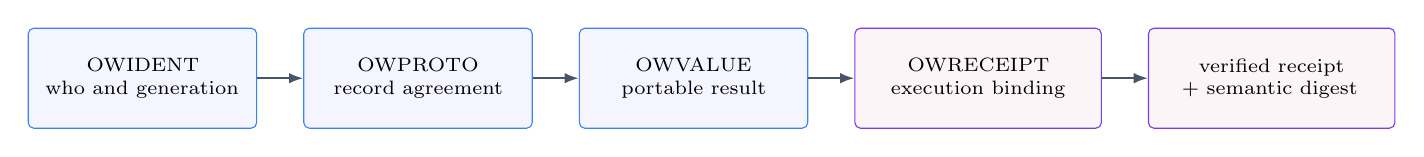
\begin{tikzpicture}[
  node distance=0.23in,
  n/.style={draw=OBlue,rounded corners=2pt,fill=blue!4,
    text width=1.05in,minimum height=0.50in,align=center,font=\scriptsize},
  r/.style={draw=OPurple,rounded corners=2pt,fill=purple!4,
    text width=1.14in,minimum height=0.50in,align=center,font=\scriptsize},
  a/.style={-{Latex[length=1.8mm]},thick,color=OSlate}
]
  \node[n] (ident) {OWIDENT\\who and generation};
  \node[n,right=of ident] (proto) {OWPROTO\\record agreement};
  \node[n,right=of proto] (value) {OWVALUE\\portable result};
  \node[r,right=of value] (receipt) {OWRECEIPT\\execution binding};
  \node[r,right=of receipt] (verify) {verified receipt\\+ semantic digest};
  \foreach \x/\y in {ident/proto,proto/value,value/receipt,receipt/verify}
    {\draw[a] (\x) -- (\y);}
\end{tikzpicture}
\caption{The World formats compose identity, protocol, portable value, and
signed execution evidence while retaining separate canonical envelopes.}
\label{fig:world-codecs}
\end{figure}

\src{crates/ostadix-api/src/world/identity_wire.rs}{18--39}
\src{crates/ostadix-api/src/world/identity_wire.rs}{62--77}
\src{crates/ostadix-api/src/world/identity_wire.rs}{98--249}
\src{crates/ostadix-api/src/world/protocol.rs}{10--12}
\src{crates/ostadix-api/src/world/protocol.rs}{148--212}
\src{crates/ostadix-api/src/world/codec.rs}{17--55}
\src{crates/ostadix-api/src/world/codec.rs}{67--115}
\src{crates/ostadix-api/src/world/codec.rs}{118--233}
\src{crates/ostadix-api/src/world/value_codec.rs}{1--6}
\src{crates/ostadix-api/src/world/value_codec.rs}{22--51}
\src{crates/ostadix-api/src/world/value_codec.rs}{88--143}
\src{crates/ostadix-api/src/world/value_codec.rs}{221--340}
\src{crates/ostadix-api/src/world/receipt.rs}{1--6}
\src{crates/ostadix-api/src/world/receipt.rs}{20--28}
\src{crates/ostadix-api/src/world/receipt.rs}{600--769}
\src{crates/ostadix-api/src/world/receipt.rs}{806--839}
\src{crates/ostadix-api/src/world/receipt_codec.rs}{27--40}
\src{crates/ostadix-api/src/world/receipt_codec.rs}{56--131}
\src{crates/ostadix-api/src/world/receipt_codec.rs}{152--227}
\src{crates/ostadix-api/src/world/receipt_codec.rs}{230--326}

\section{Hosted surface language}
\label{sec:syntax}

\subsection{Implemented structural grammar}

The implementation AST has five semantic forms:
\texttt{RawText}, \texttt{VarRef}, \texttt{LetBinding},
\texttt{TypedExpr}, and \texttt{Call}. \src{crates/ostadix-api/src/parser.rs}{22--59}
The following EBNF is an implementation-oriented summary; context rules below
are part of the grammar.

\begin{lstlisting}[style=plaincode]
cli_source   ::= [ shebang newline ] document
shebang      ::= "#!" raw_line
document     ::= sequence
sequence     ::= { comment | raw | var | typed | binding | call }

typed        ::= raw_tag "^(" body ")_" raw_tag
raw_tag      ::= ident [ "[" uint "]" ] [ attributes ]
attributes   ::= "{" attribute { "," attribute } "}"
attribute    ::= ident | ident "=" visible_value
visible_value ::= visible_attr_char { visible_attr_char }

var          ::= "$" ident
binding      ::= "let" ident "=" ( typed | call )
call         ::= ident "(" [ call_arg { "," call_arg } ] ")"
call_arg     ::= var | call
comment      ::= "#" { non_newline_byte } [ newline ]

ident        ::= ( letter | "_" ) { letter | digit | "_" }
uint         ::= digit { digit }
letter       ::= "A"..."Z" | "a"..."z"
digit        ::= "0"..."9"
\end{lstlisting}

\texttt{visible\_attr\_char} is visible ASCII excluding braces, comma, and
equals. \texttt{raw} is one or more source bytes up to the next unescaped
structural token recognized in the current context; \texttt{raw\_line} and
\texttt{non\_newline\_byte} end at LF or CR/LF. At document level and inside
\texttt{O} or \texttt{quote}, the recognized tokens are comments, bindings,
calls, variables, and registered typed openers. Inside every other evaluator
body, only variables and registered typed openers are structural. A backslash
escapes an otherwise structural opener, closer, or variable splice. The CLI
entrypoints strip one leading shebang before invoking the parser.

\subsubsection{Exact tag symmetry}

The parser closes a typed expression only when its language, environment, and
attribute text exactly reproduce the opener. This lexical symmetry makes the
extent of every evaluator invocation locally decidable, even when foreign
source contains parentheses of its own. A missing environment is represented
internally by \texttt{u32::MAX} and selects a fresh ephemeral actor. An
explicit \texttt{LANG[n]} selects a persistent evaluator actor. Language
aliases canonicalize in the AST, and reconstruction emits the canonical form.
\src{crates/ostadix-api/src/parser.rs}{590--738} \src{crates/ostadix-api/src/parser.rs}{1030--1120}

\subsubsection{Structural versus opaque contexts}

\texttt{\$name} and registered nested typed blocks are recognized throughout
foreign bodies. The sequencing forms \texttt{let}, calls, and \texttt{\#}
comments are recognized at document level and inside \texttt{O} and
\texttt{quote}. Everywhere else, the parser preserves backend source
verbatim. Registry membership therefore controls which apparent tag forms
become structural nodes, while ordinary backend syntax retains its native
meaning. \src{crates/ostadix-api/src/parser.rs}{6--20}
\src{crates/ostadix-api/src/parser.rs}{215--410}

\subsubsection{Intentional smallness}

O delegates literal construction and ordinary computation to its evaluators.
A binding right-hand side is a typed block or call, and a call argument is a
variable load or nested call. Every resulting value therefore has an explicit
origin in an evaluator or orchestration builtin, which keeps the host grammar
small while preserving the full expression systems of its member languages.
\src{crates/ostadix-api/src/parser.rs}{412--561}

\subsection{First example: evaluator-indexed expressions}

\begin{lstlisting}[style=ostyle]
html^(
  <p>The answer is python^(
__oval_result__ = sum(x*x for x in range(10))
)_python.</p>
)_html
\end{lstlisting}

The inner Python evaluator produces a typed result. Before the outer HTML
backend runs, the runtime renders that result according to HTML's splice
rules. The splice is a first-class child node with its own evaluator identity,
environment, result type, and data dependency. This is the central syntactic
move: foreign source remains idiomatic while cross-language composition is
visible to parsing, planning, and scheduling.

\begin{figure}[htbp]
\centering
\resizebox{\linewidth}{!}{%
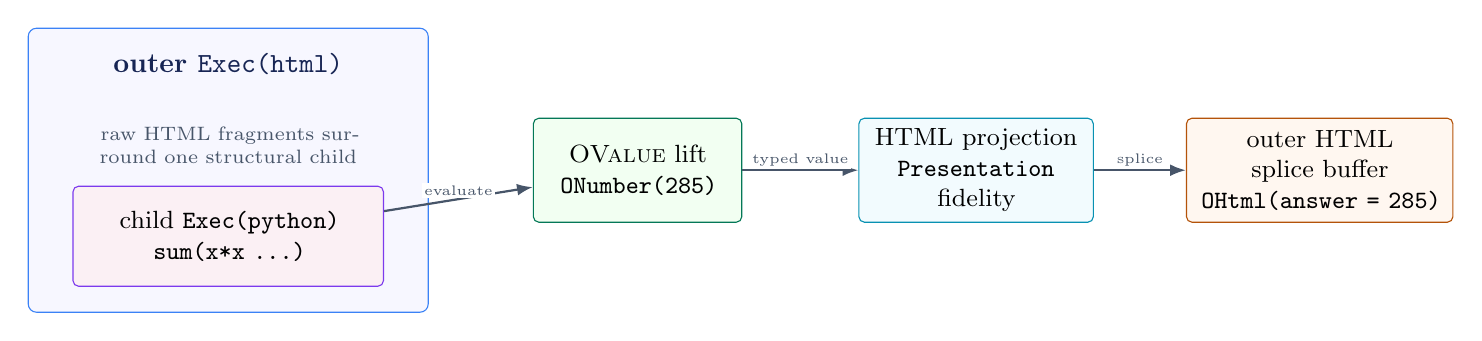
\begin{tikzpicture}[
  every node/.style={font=\small},
  outer/.style={draw=OBlue,rounded corners=3pt,fill=blue!3,
    minimum width=2.00in,minimum height=1.42in,align=center},
  inner/.style={draw=OPurple,rounded corners=2pt,fill=purple!6,
    text width=1.46in,minimum height=0.50in,align=center},
  value/.style={draw=OGreen,rounded corners=2pt,fill=green!5,
    text width=0.95in,minimum height=0.52in,align=center},
  project/.style={draw=OCyan,rounded corners=2pt,fill=cyan!5,
    text width=1.08in,minimum height=0.52in,align=center},
  result/.style={draw=OAmber,rounded corners=2pt,fill=orange!6,
    text width=1.24in,minimum height=0.52in,align=center},
  arr/.style={-{Latex[length=2mm]},thick,color=OSlate}
]
  \node[outer] (html) {};
  \node[font=\bfseries\color{ONavy},anchor=north] at
    ([yshift=-0.08in]html.north) {outer \texttt{Exec(html)}};
  \node[inner,anchor=south] (python) at
    ([yshift=0.13in]html.south) {child \texttt{Exec(python)}\\
      \texttt{sum(x*x ...)} };
  \node[font=\scriptsize\color{OSlate},text width=1.76in,align=center,anchor=south] at
    ([yshift=0.70in]html.south) {raw HTML fragments surround one structural child};

  \node[value,right=0.52in of html] (oval) {\ovalue{} lift\\
    \texttt{ONumber(285)}};
  \node[project,right=0.58in of oval] (renderer) {HTML projection\\
    \texttt{Presentation} fidelity};
  \node[result,right=0.46in of renderer] (source) {outer HTML splice buffer\\
    \texttt{OHtml(answer = 285)}};

  \draw[arr] (python) -- node[above,font=\tiny,fill=white,inner sep=1pt]
    {evaluate} (oval);
  \draw[arr] (oval) -- node[above,font=\tiny,fill=white,inner sep=1pt]
    {typed value} (renderer);
  \draw[arr] (renderer) -- node[above,font=\tiny,fill=white,inner sep=1pt]
    {splice} (source);
\end{tikzpicture}
}
\caption{A nested evaluator is a typed child in the program tree. Its result
crosses the evaluator boundary as \ovalue{}, then the receiving inline HTML
projection assembles the outer \texttt{OHtml} value.}
\label{fig:nested-evaluator}
\end{figure}

\subsection{Bindings and dependencies}

\begin{lstlisting}[style=ostyle]
let answer = python^(
__oval_result__ = 40 + 2
)_python

python^(
__oval_result__ = $answer + 1
)_python
\end{lstlisting}

\texttt{let} lowers to \texttt{Store}; \texttt{\$answer} lowers to
\texttt{Load}. Plan construction connects the load to the most recent visible
store with an explicit data edge. Each shim also receives the complete visible
scope. The first mechanism makes dependencies schedulable; the second lets
callbacks and backend adapters inspect the same lexical state that the host
used to construct the invocation.
\src{crates/ostadix-api/src/ir.rs}{760--991} \src{crates/ostadix-api/src/eval.rs}{2818--3118}

\Needspace{9\baselineskip}
\subsection{Persistent and ephemeral evaluators}

\begin{lstlisting}[style=ostyle]
python[0]^(
x = 40
)_python[0]

python[0]^(
__oval_result__ = x + 2
)_python[0]
\end{lstlisting}

Both blocks share the same language, explicit environment ID, and process
policy, so the process registry reuses one actor and Python state persists.
Bare \texttt{python\string^(...\string)\_python} blocks each receive a fresh
ephemeral identity and are cleaned up after execution. Different numeric IDs
isolate interpreter-local state; ambient \texttt{HostWorld} resources remain
shared. \src{crates/ostadix-api/src/process.rs}{1480--2129}

\begin{claimbox}[Two explicit state domains]
Root \texttt{Store} nodes commit to the caller's O scope, and nested stores
belong to the nested evaluation scope. Persistent evaluator actors retain the
backend's own process state under their environment identity. This separation
gives O lexical state a graph-visible lifetime while allowing a backend such
as Python to preserve its native runtime state across selected invocations.
\end{claimbox}

\begin{figure}[htbp]
\centering
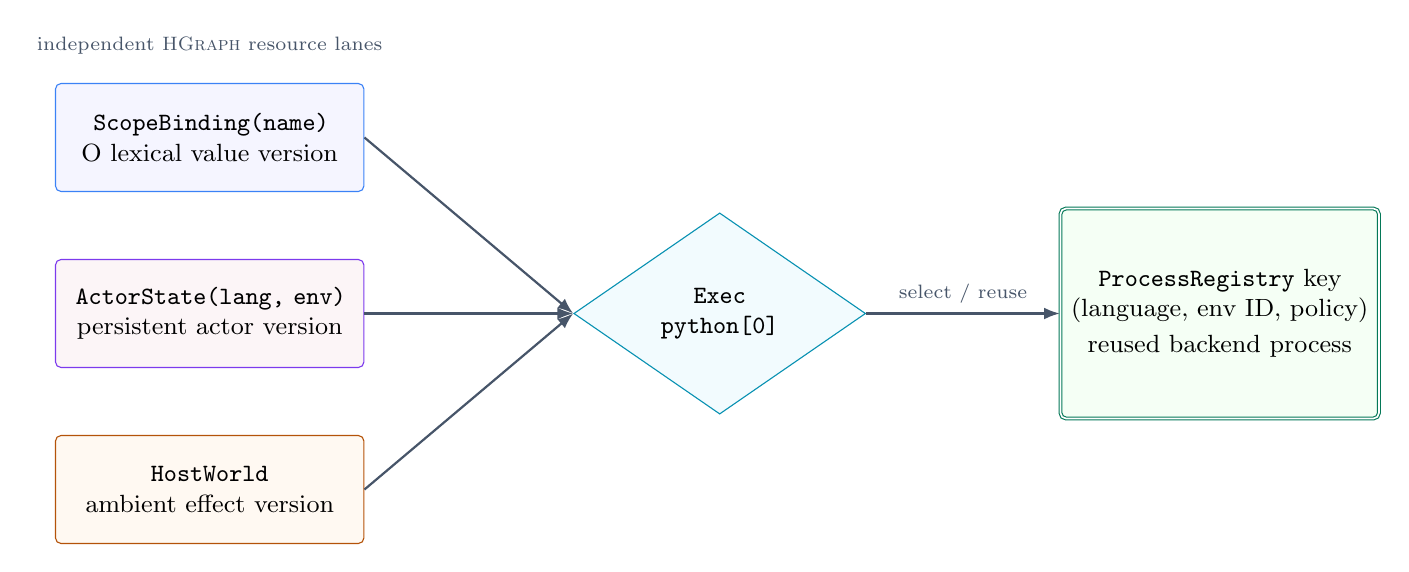
\begin{tikzpicture}[
  x=1in,y=1in,
  every node/.style={font=\small},
  scope/.style={draw=OBlue,rounded corners=2pt,fill=blue!4,
    text width=1.45in,minimum height=0.54in,align=center},
  actor/.style={draw=OPurple,rounded corners=2pt,fill=purple!4,
    text width=1.45in,minimum height=0.54in,align=center},
  world/.style={draw=OAmber,rounded corners=2pt,fill=orange!5,
    text width=1.45in,minimum height=0.54in,align=center},
  exec/.style={diamond,aspect=1.45,draw=OCyan,fill=cyan!5,
    text width=1.02in,align=center,inner sep=1pt},
  process/.style={draw=OGreen,double,rounded corners=2pt,fill=green!4,
    text width=1.50in,minimum height=1.05in,align=center},
  arr/.style={-{Latex[length=2mm]},thick,color=OSlate}
]
  \node[scope] (scope) at (0,0.88) {\texttt{ScopeBinding(name)}\\O lexical value version};
  \node[actor] (actor) at (0,0) {\texttt{ActorState(lang, env)}\\persistent actor version};
  \node[world] (world) at (0,-0.88) {\texttt{HostWorld}\\ambient effect version};
  \node[exec] (exec) at (2.55,0) {\texttt{Exec}\\\texttt{python[0]}};
  \node[process] (process) at (5.05,0) {\texttt{ProcessRegistry} key\\
    (language, env ID, policy)\\[2pt]reused backend process};

  \draw[arr] (scope.east) -- (exec.west);
  \draw[arr] (actor.east) -- (exec.west);
  \draw[arr] (world.east) -- (exec.west);
  \draw[arr] (exec.east) -- node[above,font=\scriptsize] {select / reuse} (process.west);
  \node[font=\scriptsize\color{OSlate}] at (0,1.34)
    {independent \hgraph{} resource lanes};
\end{tikzpicture}
\caption{Lexical bindings, persistent actor state, and ambient host effects
remain separate graph resources. \texttt{ActorState} uses canonical language
and environment identity; concrete process reuse additionally includes the
sandbox policy.}
\label{fig:state-domains}
\end{figure}

\section{Hosted dynamic semantics}
\label{sec:semantics}

\subsection{Evaluation order}

The default public path strips a shebang, parses the document, lowers it, and
executes the graph. \texttt{O\_EXECUTOR=serial} selects the reference
interpreter; \texttt{graph} is the default. The graph executor preserves
required data, sequence, completion, and resource-state dependencies.
\src{src/main.rs}{15--315} \src{crates/ostadix-api/src/eval.rs}{726--763}

At document level, evaluation returns the last non-null root result. Raw
regions preserve backend source. A typed block:

\begin{enumerate}
  \item evaluates structural children and loads visible bindings;
  \item renders child values using the selected backend's splice renderer;
  \item resolves an inline evaluator or an external backend actor;
  \item sends source, environment identity, bindings, and policy;
  \item decodes the backend result into \ovalue{}.
\end{enumerate}

\subsection{Quotation and meta-evaluation}

\texttt{quote} returns an unevaluated \texttt{OExpr}. A Python shim can invoke
\texttt{O.eval(expr)}, which reparses and lowers the quoted form under a cloned
callback scope. \texttt{O.scope(map)} constructs an explicit detached scope,
and the two-argument \texttt{O.eval(expr, scope)} form chooses it.
\src{crates/ostadix-api/src/eval.rs}{2039--2087} \src{crates/ostadix-api/src/eval.rs}{2938--3118}

\begin{lstlisting}[style=ostyle]
python[0]^(
q = quote^(python^(6 * 7)_python)_quote
__oval_result__ = O.eval(q)
)_python[0]
\end{lstlisting}

The callback path clones or explicitly selects an O scope, reparses the quoted
expression, and sends its result back through the waiting actor protocol.
Actor identity also provides a deadlock guard: an actor waiting on its own
callback rejects recursive re-entry. Deferred shim forcing follows a
single-level process path. \src{crates/ostadix-api/src/eval.rs}{1875--1987}
\src{crates/ostadix-api/src/process.rs}{919--929}

\subsection{Demand policies and requests}

The evaluator exposes three demand policies:

\begin{longtable}{P{0.18\textwidth} P{0.35\textwidth} P{0.39\textwidth}}
\toprule
\textbf{Policy} & \textbf{Effect} & \textbf{Resolution rule} \\
\midrule
\endhead
Eager &
Resolve normal calls and blocks immediately. &
The ordinary document policy. \\
Lazy &
Construct a request or cache-safe deferred value. &
\texttt{\{lazy\}} is accepted only for trusted inline renderers whose
fingerprint covers the relevant inputs. \\
Autonomous &
Buffer eligible requests for scheduler resolution. &
Strict cache behavior can turn a missing result into an error after flush. \\
\bottomrule
\end{longtable}

\texttt{\{defer\}} captures an evaluator request for explicit forcing with
\texttt{now}; its request remains non-cacheable, and an unforced splice is a
typed evaluation error. \texttt{\{lazy\}} attaches a cache-safety contract to
trusted inline evaluation, so the runtime can force it on demand and reuse the
fingerprinted result.
\src{crates/ostadix-api/src/execution_contract.rs}{83--162}
\src{crates/ostadix-api/src/execution_contract.rs}{218--285}
\src{crates/ostadix-api/src/eval.rs}{1875--2022}
\src{crates/ostadix-api/src/eval.rs}{2874--2924}

Autonomous resolution is a fingerprint-keyed, two-level scheduler. It first
collects the transitive request closure and deduplicates the DAG, promotes
results through an L1 memory cache and an L2 JSON disk cache, then dispatches
uncached ready nodes in topological waves. Default parallelism is the smaller
of the available CPU count and eight, with an explicit caller override. The L2
path resolves through \texttt{XDG\_CACHE\_HOME}, then \texttt{HOME}, then the
platform temporary directory. Each cache entry is written beside its final
path and atomically renamed. A missing, unreadable, malformed, or unwritable
cache entry is a soft cache event: execution proceeds and preserves the result
contract. \src{crates/ostadix-api/src/scheduler.rs}{1--38}
\src{crates/ostadix-api/src/scheduler.rs}{76--147}
\src{crates/ostadix-api/src/scheduler.rs}{233--350}

The Nix request ladder is explicit:

\[
\texttt{NixExpr}
\xrightarrow{\ \texttt{instantiate}\ }
\texttt{Derivation}
\xrightarrow{\ \texttt{realise}\ }
\texttt{StorePath}
\xrightarrow{\ \texttt{activate}\ }
\texttt{System}.
\]

\texttt{dry\_activate} constructs a preview request,
\texttt{activate(path)} performs the ambient-authority activation, and
\texttt{current\_system} produces a referential system value. Separate request
constructors make inspection and state-changing activation distinct in the
value algebra and scheduler.

The perform boundary is concrete. \texttt{instantiate} wraps the source as
\texttt{(let v = (BODY); in v.drvPath)}, runs
\texttt{nix eval --raw --impure --expr}, validates the returned
\texttt{/nix/store/*.drv} path, and asks \texttt{nix derivation show} for its
output names, using \texttt{out} when output inspection fails. \texttt{realise}
runs \texttt{nix build DRV\string^out --no-link --print-out-paths} and validates the
printed store path. Activation executes the closure's
\texttt{bin/switch-to-configuration} with \texttt{switch} or
\texttt{dry-activate} and supplies the chosen profile in \texttt{NIX\_PROFILE}.
\src{crates/ostadix-api/src/eval.rs}{3167--3340}
\src{crates/ostadix-api/src/nix_ops.rs}{33--145}
\src{crates/ostadix-api/src/nix_ops.rs}{176--258}
\src{crates/ostadix-api/src/nixos_ops.rs}{29--101}

\subsection{Coordination groups}

\begin{longtable}{P{0.16\textwidth} P{0.40\textwidth} P{0.36\textwidth}}
\toprule
\textbf{Mode} & \textbf{Settlement} & \textbf{Current behavior} \\
\midrule
\endhead
\texttt{batch} &
Collect every outcome in member order; failures become structured error
values. &
Threadable work respects scheduler parallelism. \\
\texttt{all} &
Require every member to succeed; otherwise fail the group. &
Threadable work respects scheduler parallelism. \\
\texttt{any} &
Return the first success; fail only when all fail. &
Probe serial members in source order; if none succeeds, launch the complete
threadable cohort. \\
\texttt{race} &
Return the first settlement, success or failure. &
The first serial member settles the group when one is present; otherwise race
the complete threadable cohort. \\
\bottomrule
\end{longtable}

Group constructors capture unevaluated arguments, preserving their computation
topology until group resolution. Only Nix-family requests are classified as
threadable in the group path; arbitrary shim evaluation remains serial.
\src{crates/ostadix-api/src/eval.rs}{1540--1873}

\begin{claimbox}[Two concurrency planes]
Graph-level parallelism is derived from value, completion, and resource
dependencies, then admitted for verified-safe inline operations. Group-level
concurrency is selected explicitly by \texttt{batch}, \texttt{all},
\texttt{any}, or \texttt{race} and currently dispatches the threadable Nix
request family. One plane extracts parallel work from program structure; the
other gives the program an explicit settlement topology.
\end{claimbox}

\section{The OValue semantic boundary}
\label{sec:ovalue}

\ovalue{} is the cross-evaluator tagged algebra. It carries values, references,
control objects, and error information across runtimes.
\src{crates/ostadix-api/src/value.rs}{679--986}

\begin{figure}[htbp]
\centering
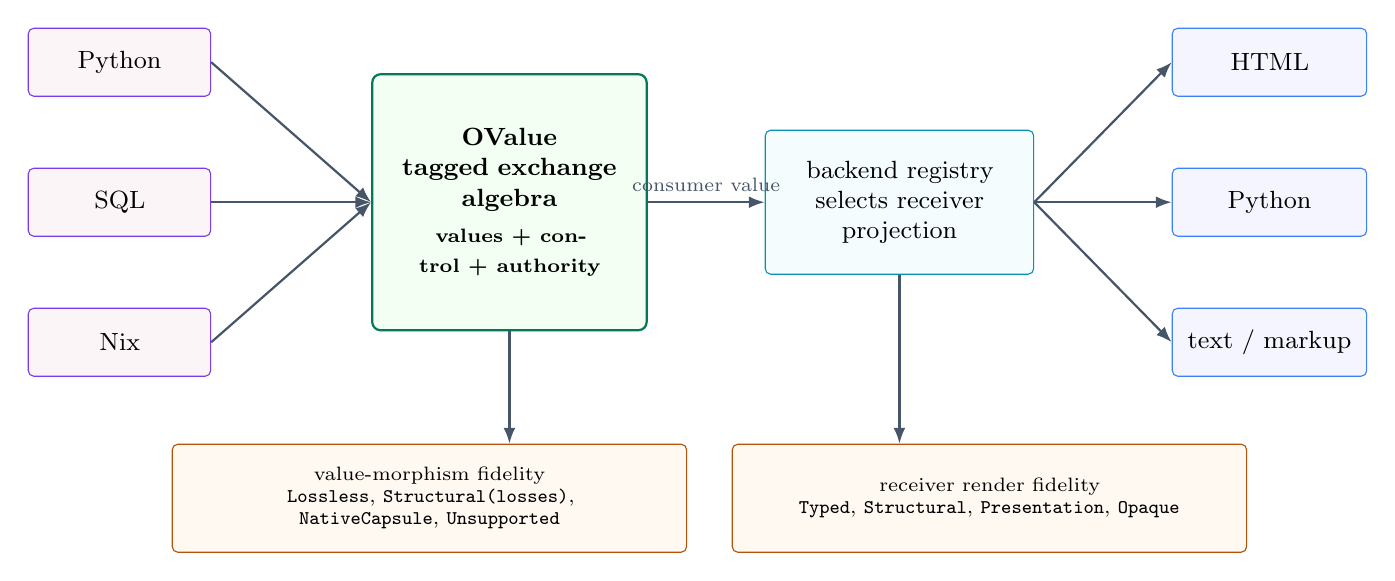
\begin{tikzpicture}[
  x=1in,y=1in,
  every node/.style={font=\small},
  producer/.style={draw=OPurple,rounded corners=2pt,fill=purple!4,
    text width=0.82in,minimum height=0.34in,align=center},
  hub/.style={draw=OGreen,rounded corners=3pt,fill=green!5,line width=0.8pt,
    text width=1.28in,minimum height=1.28in,align=center},
  registry/.style={draw=OCyan,rounded corners=2pt,fill=cyan!4,
    text width=1.25in,minimum height=0.72in,align=center},
  consumer/.style={draw=OBlue,rounded corners=2pt,fill=blue!4,
    text width=0.88in,minimum height=0.34in,align=center},
  fidelity/.style={draw=OAmber,rounded corners=2pt,fill=orange!5,
    text width=2.48in,minimum height=0.54in,align=center,font=\scriptsize},
  arr/.style={-{Latex[length=2mm]},thick,color=OSlate}
]
  \node[producer] (py) at (0,0.70) {Python};
  \node[producer] (sql) at (0,0) {SQL};
  \node[producer] (nix) at (0,-0.70) {Nix};
  \node[hub] (oval) at (1.95,0) {\bfseries\ovalue{}\\tagged exchange\\algebra\\[2pt]
    \scriptsize values + control + authority};
  \node[registry] (registry) at (3.90,0) {backend registry\\selects receiver\\projection};
  \node[consumer] (html) at (5.75,0.70) {HTML};
  \node[consumer] (python) at (5.75,0) {Python};
  \node[consumer] (text) at (5.75,-0.70) {text / markup};
  \node[fidelity] (morphism) at (1.55,-1.48) {value-morphism fidelity\\
    \texttt{Lossless}, \texttt{Structural(losses)},
    \texttt{NativeCapsule}, \texttt{Unsupported}};
  \node[fidelity] (rendering) at (4.35,-1.48) {receiver render fidelity\\
    \texttt{Typed}, \texttt{Structural},
    \texttt{Presentation}, \texttt{Opaque}};

  \foreach \p in {py,sql,nix} {\draw[arr] (\p.east) -- (oval.west);}
  \draw[arr] (oval) -- node[above,font=\scriptsize] {consumer value} (registry);
  \foreach \c in {html,python,text} {\draw[arr] (registry.east) -- (\c.west);}
  \draw[arr] (oval.south) -- (oval.south |- morphism.north);
  \draw[arr] (registry.south) -- (registry.south |- rendering.north);
\end{tikzpicture}
\caption{Every producer lifts into one inspectable algebra. The receiving
backend then projects that value into its own source domain. Value conversion
and source rendering retain distinct, composable fidelity judgments.}
\label{fig:ovalue-hub}
\end{figure}

\begin{longtable}{P{0.20\textwidth} P{0.72\textwidth}}
\toprule
\textbf{Family} & \textbf{Implemented variants} \\
\midrule
\endhead
Scalars &
Null, Bool, Number, Text, Char, HTML, store paths, and expressions. \\
Numbers &
Arbitrary-precision integers, rationals, decimals including special values, binary
floats, arbitrary-precision floats, and complex numbers. \\
Collections &
List, Map, Seq, Object, entry-preserving map, Set, Symbol, and Keyword. \\
Rich payloads &
Blob, Bytes, Graph, and Native capsule. \\
Execution state &
Scope, Snapshot, Thunk, Request, Group, structured Error. \\
World references &
NixExpr, Derivation, System, Capability. \\
\bottomrule
\end{longtable}

The public subalgebras make collection shape, authority, snapshots, native
rehydration, and runtime persistence explicit:

\begin{longtable}{P{0.24\textwidth} P{0.68\textwidth}}
\toprule
\textbf{Subalgebra} & \textbf{Variants} \\
\midrule
\endhead
\texttt{SeqKind} & List, Tuple, Vector. \\
\texttt{SetKind} & Ordered, Unordered. \\
\texttt{CapabilityKind} & File, MemoryRegion, Device, Clock,
NetworkEndpoint, Process, Service, SystemActivation, BackendExecution. \\
\texttt{SnapshotKind} & System, Service, Filesystem, Device. \\
\texttt{RequestKind} & Instantiate, Realise, Eval, Activate. \\
\texttt{NativeCodecSafety} & DataOnly, SourceBacked, UnsafeOpaque, LiveHandle. \\
\texttt{NativeBoundary} & Pure, Referential, Effectful. \\
\texttt{RehydratePolicy} & Portable, SameBackend, SameProcess, Never. \\
\texttt{RuntimeBoundary} & Pure, Referential, Effectful. \\
\texttt{Fidelity} & Lossless, Structural, NativeCapsule, Unsupported. \\
\texttt{AnnotationKind} & TypeTag, NumericPrecision, NumericExactness,
Encoding, Ordering, Identity, Constraint, Capability, Presentation, and an
extensible BackendSpecific label. \\
\bottomrule
\end{longtable}

\subsection{Authorable tagged OValue schema}

Every JSON or CBOR OValue is selected by its top-level \texttt{t} field.
Fields named as values, items, members, bindings, metadata, or state contain
OValues recursively.

\begin{longtable}{P{0.22\textwidth} P{0.70\textwidth}}
\toprule
\textbf{\texttt{t} tag} & \textbf{Fields and nested vocabulary} \\
\midrule
\endhead
\texttt{null}; \texttt{bool} & Null consists exactly of the \texttt{t} tag.
Bool adds Boolean \texttt{v}. \\
\texttt{number} & \texttt{v.kind} is
\texttt{int\{v\}}, \texttt{rational\{num,den\}},
\texttt{decimal\{coeff,exp10,special?\}},
\texttt{binary\_float\{format,bits\}},
\texttt{big\_float\{mantissa,exp2,precision?,special?\}}, or
\texttt{complex\{re,im\}}. A question mark identifies an optional or nullable
field. Canonical big integers are decimal strings;
formats are \texttt{f32}|\texttt{f64}; specials are \texttt{nan},
\texttt{pos\_inf}, \texttt{neg\_inf}, \texttt{pos\_zero}, and
\texttt{neg\_zero}. \\
\texttt{text}; \texttt{char}; \texttt{html}; \texttt{store\_path};
\texttt{expr} & Text has \texttt{v\{utf8,encoding?\}}; char has
\texttt{scalar}; HTML has \texttt{v}; store path has \texttt{path}; expression
has \texttt{src}. \\
\texttt{list}; \texttt{map} & List \texttt{v} is an array; map \texttt{v} is
a string-keyed object. \\
\texttt{seq}; \texttt{object}; \texttt{entries\_map}; \texttt{set} & Seq has
\texttt{kind=list|tuple|vector} and \texttt{items}; object has string
\texttt{fields}; entries-map has an \texttt{entries} array of key/value pairs;
set has \texttt{kind=ordered|unordered} and \texttt{items}. \\
\texttt{symbol}; \texttt{keyword}; \texttt{scope} & Symbol and keyword
\texttt{v} each contain optional or nullable \texttt{namespace} and required
\texttt{name}; scope has string-keyed \texttt{bindings}. \\
\texttt{blob}; \texttt{bytes} & Blob has base64 \texttt{v} and \texttt{mime}.
Bytes has \texttt{v\{bytes,media\_type\}}, with an octet array and nullable
media type. \\
\texttt{graph} & \texttt{root} is a node ID; \texttt{nodes} contain
\texttt with \texttt{value}, or \texttt with
\texttt{target}. \\
\texttt{native} & \texttt{v} contains \texttt{lang}, nullable
\texttt{implementation}/\texttt{version}, \texttt{type\_name},
\texttt{identity\{stable?,live?\}}, \texttt{codec}, optional or nullable byte
\texttt{payload}, \texttt{boundary}, \texttt{safety},
\texttt{capabilities}, \texttt{metadata}, and \texttt{rehydrate}. Boundary is
\texttt{pure|referential|effectful}; safety is
\texttt{data\_only|source\_backed|unsafe\_opaque|live\_handle}; rehydration is
\texttt{portable|same\_backend|same\_process|never}. \\
\texttt{nix\_expr}; \texttt{derivation} & Nix expression has \texttt{body},
\texttt{deps}, and \texttt{fingerprint}; derivation has \texttt{drv\_path},
\texttt{outputs}, and \texttt{deps}. \\
\texttt{request}; \texttt{system} & Request has \texttt{kind},
\texttt{source}, and \texttt{fingerprint}. Kind is \texttt{instantiate},
\texttt{realise}, an \texttt{eval} object with \texttt{lang},
\texttt{env\_id}, \texttt{cacheable}, nullable \texttt{authority}, and
\texttt{permissions}, or an \texttt{activate} object with \texttt{profile},
\texttt{dry\_run}, and nullable \texttt{authority}. System has
\texttt{profile\_path}. \\
\texttt{capability}; \texttt{snapshot} & Capability has \texttt{kind}, opaque
\texttt{identity}, and descriptive \texttt{metadata}. Snapshot has
\texttt{kind=system|service|filesystem|device}, \texttt{identity}, and
\texttt{state}. \\
\texttt{thunk}; \texttt{group}; \texttt{error} & Thunk has \texttt{body},
\texttt{deps}, and \texttt{fingerprint}. Group has
\texttt{mode=batch|all|any|race}, \texttt{members}, and \texttt{fingerprint}.
Error has \texttt{msg}. \\
Legacy input tags & \texttt{int\{v\}}, \texttt{float\{v\}}, and
\texttt{str\{v\}} are accepted and normalize to canonical number or text. \\
\bottomrule
\end{longtable}

Capability kinds are \texttt{file}, \texttt{memory\_region}, \texttt{device},
\texttt{clock}, \texttt{network\_endpoint}, \texttt{process},
\texttt{service}, \texttt{system\_activation}, and
\texttt{backend\_execution}. \src{crates/ostadix-api/src/value.rs}{94--663}
\src{crates/ostadix-api/src/value.rs}{679--1246}
\src{crates/ostadix-api/src/value.rs}{1257--1475}

\subsection{Fidelity}

Conversions carry one of four fidelity states:
\texttt{Lossless}, an accumulated set of structural losses,
\texttt{NativeCapsule}, or \texttt{Unsupported}. Composition terminates at a
fixpoint and preserves the weakest accumulated guarantee.
\src{crates/ostadix-api/src/value.rs}{155--547}

\texttt{BackendMorphismV1} defines bounded Python, JavaScript, and Rust
crossing profiles with explicit input projection, output injection, rejection
kinds, two fidelity legs, and a checked lossless round-trip law. Catalog V5
binds each profile to its canonical backend entry. The HGraph solver exposes
the resulting assessment beside its compatibility fidelity result in shadow
mode, making profile divergences inspectable while the established admission,
rendering, and dispatch paths retain their current authority.
\src{crates/ostadix-api/src/backend_morphism.rs}{1--7}
\src{crates/ostadix-api/src/backend_morphism.rs}{19--40}
\src{crates/ostadix-api/src/backend_morphism.rs}{126--271}
\src{crates/ostadix-api/src/backend_morphism.rs}{365--404}
\src{crates/ostadix-api/src/hgraph/solve.rs}{874--881}

\subsection{Representation-sensitive identity}

\begin{itemize}
  \item Rational identity preserves the supplied numerator, denominator, and
        sign representation after rejecting a zero denominator.
  \item Unordered sets sort canonical item encodings; ordered sets preserve
        declared order; both preserve encoded multiplicity.
  \item System identity is referential and based on profile path.
  \item Snapshot identity uses kind and referential identity, leaving changing
        snapshot state outside the stable identity key.
  \item Schema encoding preserves descriptors for capabilities, scopes,
        native handles, and host effects; their live authority remains bound
        to the runtime that owns them.
\end{itemize}

\src{crates/ostadix-api/src/value.rs}{1507--1518}
\src{crates/ostadix-api/src/value.rs}{1785--1858}
\src{crates/ostadix-api/src/value.rs}{1954--2254}
\src{crates/ostadix-api/src/value.rs}{2529--2795}

\subsection{Wire protocol}

Backend commands and responses use four-byte big-endian length-prefixed CBOR
with a 128 MiB frame limit. Map encoding is canonicalized. Decoding rejects
trailing bytes, indefinite encodings, malformed forms, non-text map keys, and
non-finite encodings outside the defined value schema.
\src{crates/ostadix-api/src/wire.rs}{1--105}
\src{crates/ostadix-api/src/canonical_cbor.rs}{1--23}
\src{crates/ostadix-api/src/canonical_cbor.rs}{49--85}
\src{crates/ostadix-api/src/canonical_cbor.rs}{157--220}

The Rust serializer emits canonical \texttt{number} and \texttt{text} frames.
Compatibility shims can emit legacy \texttt{int}, \texttt{float}, and
\texttt{str} frames; Rust decoding normalizes them into \texttt{ONumber} and
\texttt{OText} before the value enters the hosted algebra.

The complete shim-extension vocabulary is:

\begin{longtable}{P{0.24\textwidth} P{0.68\textwidth}}
\toprule
\textbf{Direction} & \textbf{Tagged CBOR body} \\
\midrule
\endhead
Runtime to shim & \texttt{cmd=exec} with \texttt{code} and a string-keyed
\texttt{bindings} map of OValues. \\
Runtime to shim & Fieldless \texttt{cmd=cleanup} and \texttt{cmd=ping}. \\
Runtime to shim & \texttt{cmd=eval\_result} with \texttt{value}. \\
Shim to runtime & \texttt{status=ok} with \texttt{value}; or
\texttt{status=err} with \texttt{message}. \\
Shim to runtime & \texttt{status=eval\_request} with \texttt{src} and optional
\texttt{scope}. The runtime evaluates that O source, returns
\texttt{eval\_result}, and the paused shim resumes until \texttt{ok} or
\texttt{err}. \\
\bottomrule
\end{longtable}
\src{crates/ostadix-api/src/value.rs}{3318--3380}

\section{Backends, actors, and authority}
\label{sec:backends}

\subsection{Static registry}

The compile-time Rust registry binds each recognized language tag to its
renderer, execution mode, cache-safety classification, and required authority.
It declares 30 canonical tags plus six aliases. Seven structural/value
handlers execute inline or as builtins; external evaluation is mediated by
native adapters and bundled compatibility shims. A single registry entry
therefore connects surface syntax to planning metadata, state support,
morphism profile, runtime requirements, and runtime dispatch.
\src{crates/ostadix-api/src/backend_catalog.rs}{623--685}
\src{crates/ostadix-api/src/backend_catalog.rs}{841--921}
\src{crates/ostadix-api/src/backend_catalog.inc.rs}{161--590}
\src{crates/ostadix-api/src/shims.rs}{7--182}

\begin{longtable}{P{0.21\textwidth} P{0.71\textwidth}}
\toprule
\textbf{Class} & \textbf{Registered canonical tags} \\
\midrule
\endhead
Structural/value &
\texttt{O}, \texttt{quote}, \texttt{nix\_expr}, \texttt{html},
\texttt{markdown}, \texttt{latex}, \texttt{text}. \\
Nix and systems tests &
\texttt{nix}, \texttt{nix\_store}, \texttt{nixos\_test},
\texttt{ubuntu\_vm}. \\
Data and scripting &
\texttt{sql}, \texttt{python}, \texttt{bash}, \texttt{shell},
\texttt{javascript}, \texttt{ruby}, \texttt{matlab},
\texttt{mathematica}. \\
Compiled and functional &
\texttt{haskell}, \texttt{ocaml}, \texttt{webassembly}, \texttt{rust},
\texttt{racket}, \texttt{csharp}, \texttt{c}, \texttt{cpp},
\texttt{lisp}, \texttt{common\_lisp}, \texttt{java}. \\
\bottomrule
\end{longtable}

The six aliases are exact parser spellings: \texttt{o} maps to \texttt{O};
\texttt{py} maps to \texttt{python}; \texttt{md} maps to
\texttt{markdown}; \texttt{tex} maps to \texttt{latex}; and
\texttt{plain} maps to \texttt{text}; \texttt{ubuntu} maps to
\texttt{ubuntu\_vm}. Block attributes attach execution
metadata directly to the evaluator-indexed form. The implemented attribute
surface is \texttt{cap=name}, the four authority flags \texttt{fs\_read},
\texttt{fs\_write}, \texttt{network}, and \texttt{process},
\texttt{lazy}, \texttt{defer},
\texttt{effects=pure|unknown}, \texttt{reads=...}, \texttt{writes=...}, and
\texttt{serial=host}. Effect-resource lists use \texttt{+} or \texttt{;} as
separators. The resource spellings are:

\begin{center}
\begin{tabular}{lll}
\texttt{project:path} & \texttt{host:path} & \texttt{env:NAME} \\
\texttt{scope:name} & \texttt{network:endpoint} & \texttt{service:name} \\
\texttt{actor:language[index]} & \texttt{evaluator} & \texttt{stdio} \\
\texttt{hostworld} & &
\end{tabular}
\end{center}

These spellings let source describe graph resources in the same vocabulary
used by the planner. \src{crates/ostadix-api/src/parser.rs}{590--738}
\src{crates/ostadix-api/src/effects.rs}{1--434}

The repeatable backend-grant syntax is
\texttt{NAME=LANG[:RIGHT,RIGHT]}. \texttt{NAME} begins with an ASCII letter or
underscore and continues with ASCII letters, digits, or underscores.
\texttt{LANG} is nonempty; known aliases canonicalize, and \texttt{*} creates
a wildcard. Parser dispatch still requires a registered source tag. Rights are
\texttt{fs\_read}, \texttt{fs\_write},
\texttt{network}, and \texttt{process}; commas separate them and duplicates
collapse. An omitted or empty rights list produces a zero-rights bearer. A
block that declares one or more authority flags uses \texttt{cap=NAME} as its
first bearer candidate. A match must contain every declared right; an absent
or insufficient binding follows the evaluator's default-authority path. The
release CLI gate executed
\texttt{runner=python:process}. \src{crates/ostadix-api/src/eval.rs}{1217--1227}
\src{tests/test_cli.sh}{888--898}

At invocation time, the adapter resolves its host executable and converts the
subset of \ovalue{} accepted by that runtime. This keeps language recognition
deterministic while allowing the executable environment to be selected by the
host installation.

\subsection{Actor process model}

Production external evaluation self-spawns the current executable in hidden
\texttt{--o-backend} mode. The process registry key is
\[
(\textit{language},\ \textit{environment ID},\ \textit{sandbox policy}).
\]
Persistent keys reuse a process; ephemeral keys are removed after evaluation.
Most backends are Rust adapters that invoke local executables. Python and
\texttt{nixos\_test} use legacy Python proxy shims. Python retains this path
for the host callback protocol used by \texttt{O.eval}.
\src{crates/ostadix-api/src/process.rs}{554--609}
\src{crates/ostadix-api/src/backend.rs}{77--743}

Backend stdout is decoded in a defined fallback order: tagged or ordinary
JSON, integer/big integer, float, then text. SQL additionally collapses a
single-row, single-column result. Environment conversion is narrower than
the full \ovalue{} universe. \src{crates/ostadix-api/src/backend.rs}{1229--1503}

\subsection{Hosted authority model}

The source contains random 256-bit bearer identities, typed backend rights
(\texttt{fs\_read}, \texttt{fs\_write}, \texttt{network},
\texttt{process}), broker checks, revocation, and policy-partitioned process
reuse. \src{crates/ostadix-api/src/capability.rs}{13--188}

The ordinary CLI executes backends with the ambient authority of the O
process. Its launch path realizes that model in five steps:

\begin{enumerate}
  \item evaluator startup mints a wildcard bearer with all four rights;
  \item source \texttt{cap=} resolution falls back to that wildcard;
  \item normal shim launch policies expand to all rights;
  \item the production Python proxy runs under the outer process policy;
  \item the macOS profile begins with \texttt{allow default} and derives
        denials from rights omitted by a narrowed embedding policy.
\end{enumerate}

\src{crates/ostadix-api/src/eval.rs}{766--796}
\src{crates/ostadix-api/src/eval.rs}{1230--1304}
\src{crates/ostadix-api/src/process.rs}{167--241}
\src{crates/ostadix-api/src/process.rs}{637--683}

\begin{claimbox}[Authority is explicit runtime state]
Hosted capability machinery supplies random bearer identity, typed rights,
revocation, policy-partitioned actor reuse, deferred-request revalidation, and
embedding hooks. The public CLI chooses the ambient policy, maximizing
backend compatibility and execution capacity. An embedding can supply a
narrowed process policy and reuse the same identity and revalidation path.
\end{claimbox}

\section{OIR, plans, effects, and HGraph execution}
\label{sec:hgraph}

\subsection{OIR is orchestration IR}

\oir{} has five node forms:

\begin{center}
\texttt{Text}\qquad
\texttt{Load}\qquad
\texttt{Store}\qquad
\texttt{Invoke}\qquad
\texttt{Exec}.
\end{center}

These forms model the complete hosted orchestration surface: source fragments,
lexical dataflow, binding publication, builtin invocation, and evaluator
execution. Lowering from the parser AST is structural; validation then turns
that representation into an executable plan. The compact vocabulary makes
every hosted construct projectable into the same graph ontology.
\src{crates/ostadix-api/src/ir.rs}{1--21}
\src{crates/ostadix-api/src/ir.rs}{78--171}

\begin{figure}[htbp]
\centering
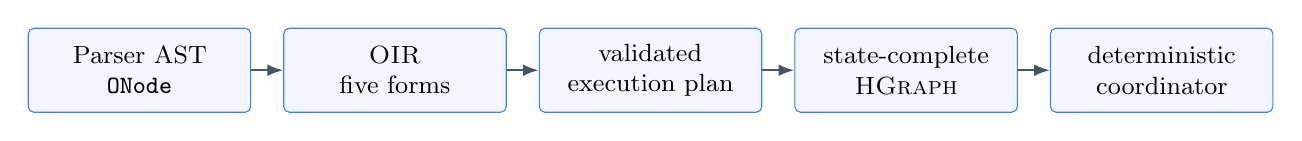
\begin{tikzpicture}[
  node distance=0.20in and 0.16in,
  n/.style={draw=OBlue,rounded corners=2pt,fill=blue!4,
    minimum height=0.42in,text width=1.02in,align=center,font=\small},
  a/.style={-{Latex[length=2mm]},thick,color=OSlate}
]
  \node[n] (ast) {Parser AST\\\texttt{ONode}};
  \node[n,right=of ast] (oir) {\oir{}\\five forms};
  \node[n,right=of oir] (plan) {validated\\execution plan};
  \node[n,right=of plan] (hg) {state-complete\\\hgraph{}};
  \node[n,right=of hg] (coord) {deterministic\\coordinator};
  \draw[a] (ast) -- (oir);
  \draw[a] (oir) -- (plan);
  \draw[a] (plan) -- (hg);
  \draw[a] (hg) -- (coord);
\end{tikzpicture}
\caption{Every ordinary hosted execution is mediated by the same lowering
seam; serial execution remains a differential oracle.}
\end{figure}

\subsection{Execution plan}

Plan node IDs are preorder-stable. Edges encode child-before-parent
structure, sibling sequencing, binding dataflow, capability dependencies, and
the full visible scope sent to shims. Each executable node freezes the
registry-derived \texttt{BackendInterface}; execution rejects an interface
that no longer matches the registry. \src{crates/ostadix-api/src/ir.rs}{540--657}
\src{crates/ostadix-api/src/ir.rs}{760--991} \src{crates/ostadix-api/src/eval.rs}{2704--2891}

\subsection{State-complete HGraph}

Each ordinary plan node maps to one value node. Every executable hyperedge
also consumes required completion tokens and versioned resource states, then
atomically produces:

\begin{enumerate}
  \item one ordinary value;
  \item one completion token;
  \item successor versions for every accessed resource.
\end{enumerate}

\begin{figure}[htbp]
\centering
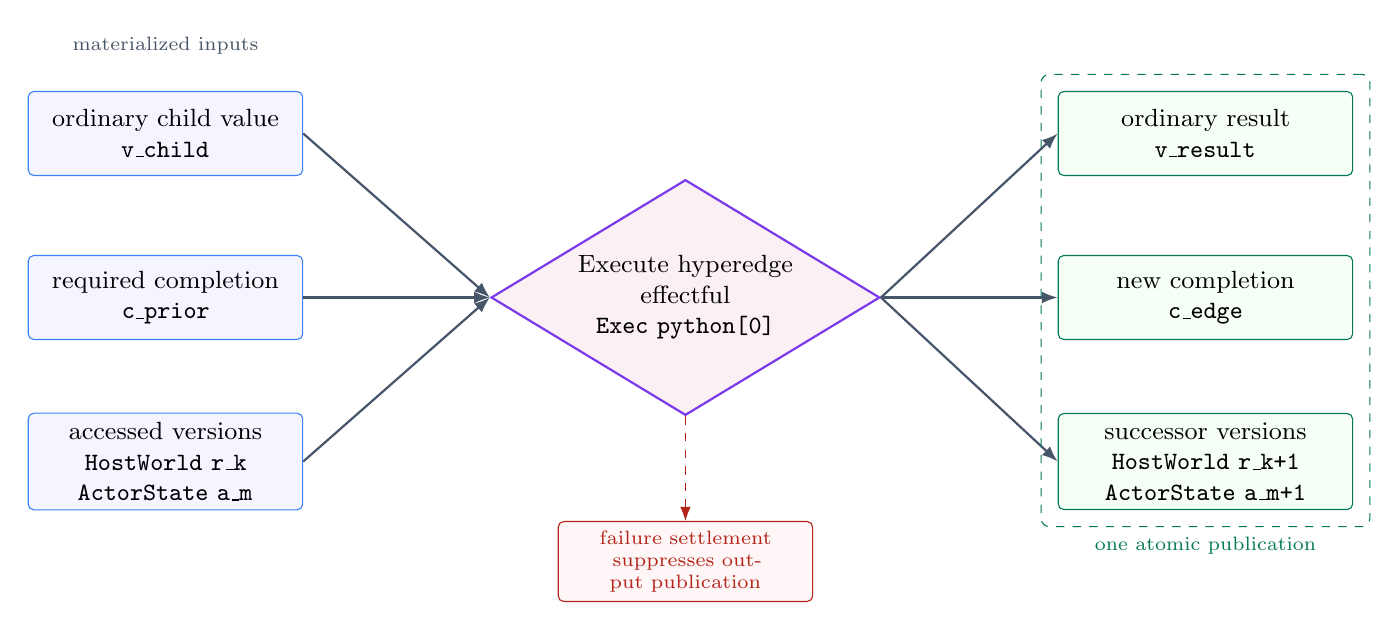
\begin{tikzpicture}[
  x=1in,y=1in,
  every node/.style={font=\small},
  input/.style={draw=OBlue,rounded corners=2pt,fill=blue!4,
    text width=1.28in,minimum height=0.42in,align=center},
  operation/.style={diamond,aspect=1.65,draw=OPurple,fill=purple!6,
    line width=0.8pt,text width=1.18in,align=center,inner sep=1pt},
  output/.style={draw=OGreen,rounded corners=2pt,fill=green!4,
    text width=1.38in,minimum height=0.42in,align=center},
  arr/.style={-{Latex[length=2mm]},thick,color=OSlate}
]
  \node[input] (valuein) at (0,0.82) {ordinary child value\\\texttt{v\_child}};
  \node[input] (donein) at (0,0) {required completion\\\texttt{c\_prior}};
  \node[input] (statein) at (0,-0.82) {accessed versions\\
    \texttt{HostWorld r\_k}\\\texttt{ActorState a\_m}};

  \node[operation] (edge) at (2.60,0) {Execute hyperedge\\effectful\\\texttt{Exec python[0]}};

  \node[output] (valueout) at (5.20,0.82) {ordinary result\\\texttt{v\_result}};
  \node[output] (doneout) at (5.20,0) {new completion\\\texttt{c\_edge}};
  \node[output] (stateout) at (5.20,-0.82) {successor versions\\
    \texttt{HostWorld r\_k+1}\\\texttt{ActorState a\_m+1}};

  \foreach \i in {valuein,donein,statein} {\draw[arr] (\i.east) -- (edge.west);}
  \foreach \o in {valueout,doneout,stateout} {\draw[arr] (edge.east) -- (\o.west);}
  \node[draw=OGreen,dashed,rounded corners=3pt,fit=(valueout)(doneout)(stateout),
    inner sep=6pt,label={[font=\scriptsize\color{OGreen}]below:one atomic publication}] {};
  \node[font=\scriptsize\color{OSlate}] at (0,1.26) {materialized inputs};
  \node[draw=ORed,rounded corners=2pt,fill=red!3,text=ORed,font=\scriptsize,
    text width=1.18in,align=center] (failure) at (2.60,-1.32)
    {failure settlement\\suppresses output publication};
  \draw[-{Latex[length=1.8mm]},dashed,color=ORed] (edge.south) -- (failure.north);
\end{tikzpicture}
\caption{An executable \hgraph{} hyperedge consumes value, completion, and
resource state together. This persistent evaluator example advances
\texttt{HostWorld} and \texttt{ActorState(python[0])}. Success publishes the
result, completion token, and every successor resource version as one graph
transition; failure withholds those graph outputs.}
\label{fig:hgraph-hyperedge}
\end{figure}

\src{crates/ostadix-api/src/hgraph/from_oir.rs}{35--291}

Validation checks unique producers, complete outputs, exact source/plan
provenance, sequence preservation, contiguous resource chains, and executable
acyclicity. The ready schedule is derived from unresolved inputs and their
producers with stable wave and ordinal ordering.
\src{crates/ostadix-api/src/hgraph/graph.rs}{368--515}
\src{crates/ostadix-api/src/hgraph/graph.rs}{1454--1908}
\src{crates/ostadix-api/src/hgraph/schedule.rs}{10--173}

\subsection{Effects and explicit resource state}

Resources include \texttt{HostWorld}, evaluator state, scope/bindings, project
and host paths, environment variables, stdio, network endpoints, services,
and actor state. Work with the general effect classification receives a
\texttt{HostWorld} dependency, serializing it against other world-mutating
operations. Source declarations add restrictions and dependencies; verified
purity is assigned by the trusted inline registry classification.
\src{crates/ostadix-api/src/effects.rs}{46--636}

Only attribute-free inline text, HTML, Markdown, and LaTeX work is treated as
verified pure and worker-eligible. Effectful ready work executes one operation
at a time in deterministic ordinal order. Successful outputs publish
atomically; the root scope commits deterministically.
\src{crates/ostadix-api/src/effects.rs}{776--843}
\src{crates/ostadix-api/src/executor/coordinator.rs}{103--1094}

\begin{claimbox}[Why the state-complete graph matters]
The graph is richer than a syntax tree because it represents value,
completion, and mutable-world dependencies separately. Its present execution
policy preserves observable equivalence and deterministic settlement while
parallelizing independently verified inline work. The same resource model
identifies the exact admission point for additional concurrent adapters: they
must declare effects precisely enough to remove unnecessary
\texttt{HostWorld} dependencies.
\end{claimbox}

\section{Projects, linking, and route policies}
\label{sec:projects}

\subsection{Project lifting and literal linking}

\texttt{o-link} has two materially different composition lanes:

\begin{itemize}
  \item A bare single directory follows the literal lane and runs the linked
        result. Explicit \texttt{--literal} emits the literal linked document;
        \texttt{--literal --run} executes it.
  \item Explicit \texttt{--project} captures a deterministic route-preserving
        project bundle. \texttt{--project --run} selects and executes a route
        through the project coordinator.
\end{itemize}

\begin{figure}[htbp]
\centering
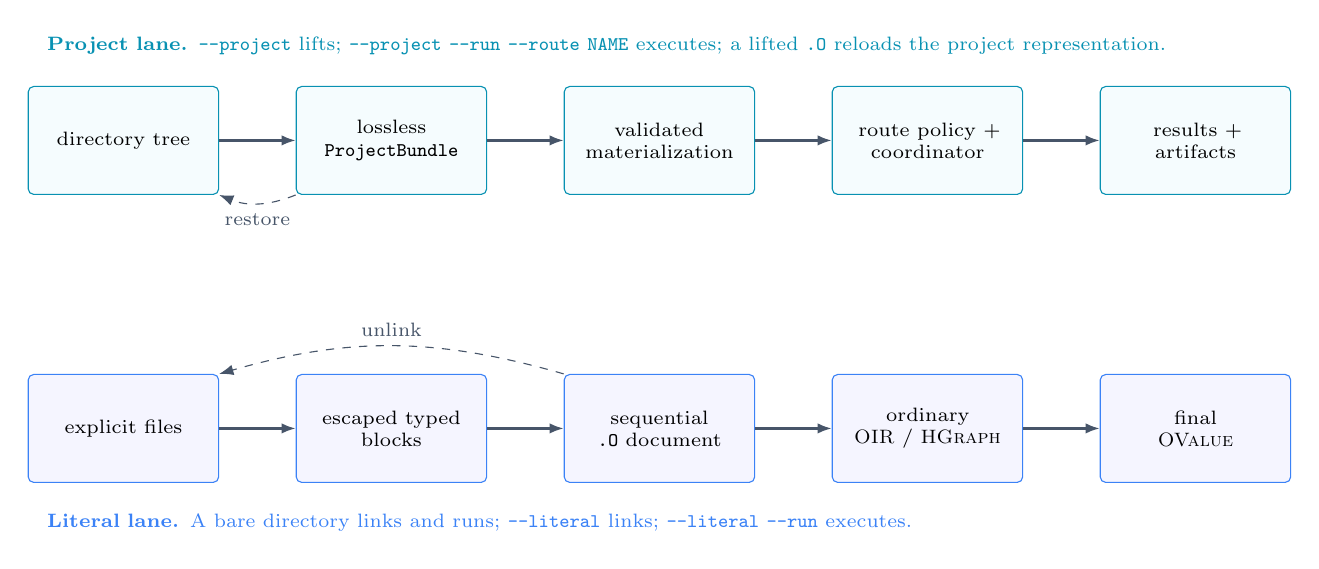
\begin{tikzpicture}[
  x=1in,y=1in,
  every node/.style={font=\scriptsize},
  project/.style={draw=OCyan,rounded corners=2pt,fill=cyan!4,
    text width=0.86in,minimum height=0.54in,align=center},
  literal/.style={draw=OBlue,rounded corners=2pt,fill=blue!4,
    text width=0.86in,minimum height=0.54in,align=center},
  arr/.style={-{Latex[length=1.8mm]},thick,color=OSlate},
  rev/.style={-{Latex[length=1.8mm]},dashed,color=OSlate}
]
  \node[font=\scriptsize\color{OCyan},text width=5.9in,align=left,
    anchor=south west] at (-0.43,1.10)
    {\textbf{Project lane.} \texttt{-{}-project} lifts;
     \texttt{-{}-project -{}-run -{}-route NAME} executes; a lifted
     \texttt{.O} reloads the project representation.};
  \node[project] (dir) at (0,0.72) {directory tree};
  \node[project] (bundle) at (1.34,0.72) {lossless\\\texttt{ProjectBundle}};
  \node[project] (workspace) at (2.68,0.72) {validated\\materialization};
  \node[project] (route) at (4.02,0.72) {route policy +\\coordinator};
  \node[project] (artifacts) at (5.36,0.72) {results +\\artifacts};

  \node[font=\scriptsize\color{OBlue},text width=5.9in,align=left,
    anchor=north west] at (-0.43,-1.10)
    {\textbf{Literal lane.} A bare directory links and runs;
     \texttt{-{}-literal} links; \texttt{-{}-literal -{}-run} executes.};
  \node[literal] (files) at (0,-0.72) {explicit files};
  \node[literal] (blocks) at (1.34,-0.72) {escaped typed\\blocks};
  \node[literal] (doc) at (2.68,-0.72) {sequential\\\texttt{.O} document};
  \node[literal] (graph) at (4.02,-0.72) {ordinary\\\oir{} / \hgraph{}};
  \node[literal] (result) at (5.36,-0.72) {final\\\ovalue{}};

  \draw[arr] (dir) -- (bundle);
  \draw[arr] (bundle) -- (workspace);
  \draw[arr] (workspace) -- (route);
  \draw[arr] (route) -- (artifacts);
  \draw[rev] (bundle.south west) to[bend left=22]
    node[below] {restore} (dir.south east);
  \draw[arr] (files) -- (blocks);
  \draw[arr] (blocks) -- (doc);
  \draw[arr] (doc) -- (graph);
  \draw[arr] (graph) -- (result);
  \draw[rev] (doc.north west) to[bend right=16]
    node[above] {unlink} (files.north east);
\end{tikzpicture}
\caption{\texttt{o-link} preserves two composition semantics. Explicit
project lift captures a reversible tree and selects whole-project routes;
literal linking constructs one hosted program and a bare single directory
runs that program by default.}
\label{fig:project-lanes}
\end{figure}

\src{src/bin/olink.rs}{183--565}
\src{src/bin/olink.rs}{841--1029}

\subsection{Compiler-emitted Project HGraph from an o-linked codebase}
\label{sec:linked-project-dot}

The tracked fixture in \path{tests/fixtures/project_hgraph/} is a complete
project codebase with one input file, a manifest, one prerequisite route, two
implementation routes, declared inputs and outputs, an environment guard, and
a \texttt{verify\_equivalent} route set named \texttt{main}. I lifted that
directory through the project form of \texttt{o-link}, asked
\texttt{olangc --target dot} to render the selected route set, and compared the
result with direct directory planning.

\begin{lstlisting}[style=plaincode]
mkdir -p output/current-master
./target/release/o-link tests/fixtures/project_hgraph --project \
    -o output/current-master/o-linked-project.O

./target/release/olangc output/current-master/o-linked-project.O \
    --target dot --route main --shim-dir backends \
    > output/current-master/o-linked-codebase-hgraph.dot

./target/release/olangc tests/fixtures/project_hgraph \
    --target dot --route main --shim-dir backends \
    > output/current-master/project-hgraph-direct.dot

cmp output/current-master/o-linked-codebase-hgraph.dot \
    output/current-master/project-hgraph-direct.dot

cp output/current-master/o-linked-codebase-hgraph.dot \
    docs/figures/o-linked-codebase-hgraph.dot
dot -Tsvg output/current-master/o-linked-codebase-hgraph.dot \
    -o docs/figures/o-linked-codebase-hgraph.svg
dot -Tpdf output/current-master/o-linked-codebase-hgraph.dot \
    -o docs/figures/o-linked-codebase-hgraph.pdf
\end{lstlisting}

The lifted artifact is 7,501 bytes with SHA-256
\breakcode{a6d97fd5b95b829c3e3a754722767960f2963e0644ba8c89da7c15d48d922bb1}.
The compiler-emitted DOT is 13,065 bytes with SHA-256
\breakcode{bf16748f53a377e950a67b9c27d48ff260dcc987a69d86c5f29ca6289df7f00b}.
The direct-directory DOT and lifted-artifact DOT are byte-identical. The SVG
is 61,756 bytes with SHA-256
\breakcode{44d7d33abf7d34ed73e3f4f37ebee77dbe5545f52cfc0077c64c021015310d01}.
The included vector PDF is 27,210 bytes with SHA-256
\breakcode{75c7d219d208a2afddc51a5c9c682c506d26cd9729145828019f88f1c6a8e90e}.

\src{tests/fixtures/project_hgraph/olang.project.toml}{1--38}
\src{src/bin/olink.rs}{713--749}
\src{src/bin/olangc.rs}{556--580}
\src{crates/ostadix-api/src/project/plan.rs}{1--25}
\src{crates/ostadix-api/src/project/plan.rs}{46--87}
\src{crates/ostadix-api/src/project/plan.rs}{91--140}

\subsubsection*{How to read the emitted graph}

The figure declares 53 semantic vertices and 62 directed edges. Twelve rose
\texttt{Execute} boxes are project operations. The other 41 vertices are
values, completion tokens, and versioned resources. Read it in seven passes:

\begin{enumerate}
  \item Begin at \texttt{Value N0}. It identifies the exact project bundle
        consumed by both alternative branches.
  \item Find \texttt{Execute E0} through \texttt{Execute E4}. This is the
        \texttt{impl-a} branch: materialize the project, build and run
        \texttt{prepare}, then build and run \texttt{impl-a}.
  \item Find \texttt{Execute E5} through \texttt{Execute E9}. This is the
        independently materialized \texttt{impl-b} branch with its own
        \texttt{prepare} prerequisite and \texttt{impl-b} execution.
  \item Follow completion diamonds from each build operation into its run
        operation. A completion edge expresses successful prerequisite
        settlement; a value edge carries an ordinary result.
  \item Follow cyan resource nodes. \texttt{HostWorld} advances from
        \texttt{@0} through \texttt{@6}; project input, build, and output
        resources advance through the operations that read or write them.
  \item Find \texttt{Execute E10}. It compares the two route results required
        by \texttt{verify\_equivalent} after both alternatives have completed.
  \item Finish at \texttt{Execute E11}. It selects the route-set result from
        the comparison outcome and publishes the final value and completion.
\end{enumerate}

The graph should be read by dependency, then by page position. Arrow labels
name the port through which a node participates:
\texttt{input:value}, \texttt{input:completion},
\texttt{input:resource-state}, \texttt{result}, \texttt{completion}, and
\texttt{resource-state}. Each \texttt{P\# ordinal \#} label binds an execute
box to its project plan operation and gives deterministic ordering among
simultaneously ready operations. A resource version belongs to the state after
the operation that produced it. A completion token belongs to the terminal
settlement of its producing operation.

\begin{figure}[htbp]
\centering
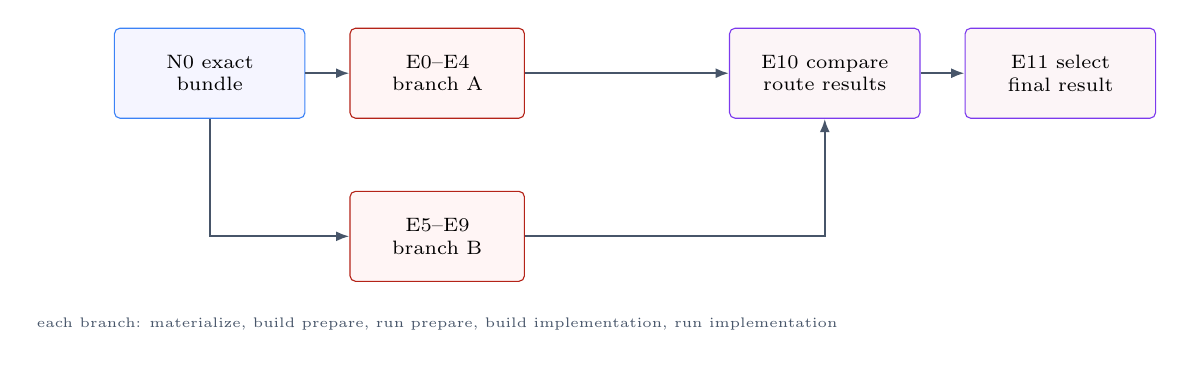
\begin{tikzpicture}[
  node distance=0.22in,
  every node/.style={font=\scriptsize},
  n/.style={draw=OBlue,rounded corners=2pt,fill=blue!4,
    text width=0.86in,minimum height=0.45in,align=center},
  e/.style={draw=ORed,rounded corners=2pt,fill=red!4,
    text width=0.78in,minimum height=0.45in,align=center},
  c/.style={draw=OPurple,rounded corners=2pt,fill=purple!4,
    text width=0.86in,minimum height=0.45in,align=center},
  a/.style={-{Latex[length=1.7mm]},thick,color=OSlate}
]
  \node[n] (bundle) {N0 exact\\bundle};
  \node[e,right=of bundle] (a0) {E0--E4\\branch A};
  \node[e,below=0.36in of a0] (b0) {E5--E9\\branch B};
  \node[c,right=1.02in of a0] (cmp) {E10 compare\\route results};
  \node[c,right=of cmp] (sel) {E11 select\\final result};
  \draw[a] (bundle) -- (a0);
  \draw[a] (bundle) |- (b0);
  \draw[a] (a0) -- (cmp);
  \draw[a] (b0) -| (cmp);
  \draw[a] (cmp) -- (sel);
  \node[font=\tiny\color{OSlate},below=0.13in of b0]
    {each branch: materialize, build prepare, run prepare, build implementation, run implementation};
\end{tikzpicture}
\caption{Reading map for the current compiler-emitted project graph. The two
source-closed alternative branches converge through comparison and final
selection.}
\label{fig:linked-reading-map}
\end{figure}

The panorama preserves the exact compiler artifact. The four detail figures
that follow it enlarge overlapping horizontal windows from that same vector
PDF. Read them from left to right. The overlap carries crossing arrows into
the next window, so a port that leaves one page can be found again at the
matching edge of the following page.

\begin{landscape}
\thispagestyle{empty}
\begin{center}
{\small\bfseries Topology index}\par
{\footnotesize\color{OSlate}Use this panorama to see branch shape and
convergence. Read node and port labels in the four enlarged panels that
follow.}\par\vspace{0.05in}

\includegraphics[width=0.98\linewidth,height=0.79\textheight,keepaspectratio]{figures/o-linked-codebase-hgraph.pdf}
\captionof{figure}{The exact directed Project HGraph emitted by
\texttt{olangc --target dot --route main} from the o-linked
\texttt{tests/fixtures/project\_hgraph} codebase. The graph contains 12 executable
operations, 41 value, completion, and resource vertices, and 62 directed
dependency edges.}
\label{fig:linked-codebase-dot}
\vfill
{\small\color{OSlate}Lee Daghlar Ostadi\hfill
Ostadix-lang Technical Whitepaper\hfill
\thepage\ / \pageref{LastPage}}
\end{center}
\end{landscape}

\begin{landscape}
\thispagestyle{empty}
\begin{center}

\includegraphics[viewport=0 0 1800 808,clip,width=0.98\linewidth,height=0.72\textheight,keepaspectratio]{figures/o-linked-codebase-hgraph.pdf}
\captionof{figure}{Project HGraph detail 1 of 4. Begin at the exact project
identity, then follow materialization and the opening operations of the
\texttt{impl-a} branch.}
\label{fig:linked-codebase-dot-detail-1}
\vfill
{\small\color{OSlate}Lee Daghlar Ostadi\hfill
Ostadix-lang Technical Whitepaper\hfill
\thepage\ / \pageref{LastPage}}
\end{center}
\end{landscape}

\begin{landscape}
\thispagestyle{empty}
\begin{center}

\includegraphics[viewport=1750 0 3570 808,clip,width=0.98\linewidth,height=0.72\textheight,keepaspectratio]{figures/o-linked-codebase-hgraph.pdf}
\captionof{figure}{Project HGraph detail 2 of 4. Complete the
\texttt{impl-a} route, then locate the independently materialized opening of
the \texttt{impl-b} branch.}
\label{fig:linked-codebase-dot-detail-2}
\vfill
{\small\color{OSlate}Lee Daghlar Ostadi\hfill
Ostadix-lang Technical Whitepaper\hfill
\thepage\ / \pageref{LastPage}}
\end{center}
\end{landscape}

\begin{landscape}
\thispagestyle{empty}
\begin{center}

\includegraphics[viewport=3520 0 5340 808,clip,width=0.98\linewidth,height=0.72\textheight,keepaspectratio]{figures/o-linked-codebase-hgraph.pdf}
\captionof{figure}{Project HGraph detail 3 of 4. Follow the build and run
operations of \texttt{impl-b}, including their completion and resource-state
ports.}
\label{fig:linked-codebase-dot-detail-3}
\vfill
{\small\color{OSlate}Lee Daghlar Ostadi\hfill
Ostadix-lang Technical Whitepaper\hfill
\thepage\ / \pageref{LastPage}}
\end{center}
\end{landscape}

\begin{landscape}
\thispagestyle{empty}
\begin{center}

\includegraphics[viewport=5290 0 7083 808,clip,width=0.98\linewidth,height=0.72\textheight,keepaspectratio]{figures/o-linked-codebase-hgraph.pdf}
\captionof{figure}{Project HGraph detail 4 of 4. Settle the second branch,
compare both route results at E10, and publish the selected route-set result at
E11.}
\label{fig:linked-codebase-dot-detail-4}
\vfill
{\small\color{OSlate}Lee Daghlar Ostadi\hfill
Ostadix-lang Technical Whitepaper\hfill
\thepage\ / \pageref{LastPage}}
\end{center}
\end{landscape}

The diagram exposes why project planning is a language operation. Directory
capture, prerequisite closure, alternative isolation, input and output
resources, equivalence comparison, and selection all become typed graph
operations. The exact-equality check shows that lifting preserves the project
semantics consumed by the compiler.

\subsection{Bundle model}

\texttt{ProjectFile} preserves relative path, raw bytes, Unix mode, symlink
metadata, evaluator hint, role, and content hash. A project carries route
specifications, guards, provenance, effects, and policy. Traversal is
deterministic and skips generated/build/cache subtrees. Materialization
validates relative paths, ancestor symlinks, and in-root symlink targets.
\src{crates/ostadix-api/src/project/model.rs}{13--290}
\src{crates/ostadix-api/src/project/bundle.rs}{28--137}
\src{crates/ostadix-api/src/project/materialize.rs}{62--179}

The bundle fingerprint covers artifact identity through paths, content hashes,
modes, and symlink flags. Route metadata remains a separately selected
execution policy. On Unix, materialization reproduces modes and symlinks from
the captured model.
\src{crates/ostadix-api/src/project/bundle.rs}{123--137}
\src{crates/ostadix-api/src/project/materialize.rs}{195--223}

Six file roles classify the captured tree: \texttt{Source}, \texttt{Asset},
\texttt{Manifest}, \texttt{GeneratedRoute}\newline\texttt{Metadata},
\texttt{Entrypoint}, and
\texttt{Other}. Route discovery proceeds in a fixed ecosystem order covering
Rust, Python, JavaScript, shell, C-family, Java, .NET, Haskell, OCaml, Nix, and
generic entrypoints. An \texttt{olang.project.toml} manifest can state exact
routes and route sets while retaining the captured files as the artifact of
record. \src{crates/ostadix-api/src/project/discover.rs}{1--132}
\src{crates/ostadix-api/src/project/manifest.rs}{1--378}

\subsection{Routes}

The native project coordinator implements \texttt{explicit},
\texttt{default}, \texttt{fallback}, \texttt{any\_success},
\texttt{race\_success}, \texttt{race\_settle}, \texttt{all},
\texttt{verify\_equivalent}, and \texttt{benchmark\_and\_select}. Alternatives
run as subprocess routes with isolated or shared workspaces as required; both
race policies cooperatively cancel losing route processes.
\src{crates/ostadix-api/src/project/model.rs}{310--402}
\src{crates/ostadix-api/src/project/runtime.rs}{2735--3240}

The project coordinator owns whole-tree materialization, route selection,
subprocess lifecycle, result settlement, and workspace sharing. Ordinary
\oir{}/\hgraph{} execution owns expression-level evaluator composition. This
division gives project routes enough context to coordinate complete build and
run alternatives while preserving the hosted language's value graph.
\src{crates/ostadix-api/src/project/manifest.rs}{40--167}
\src{crates/ostadix-api/src/project/runtime.rs}{695--704}

\begin{longtable}{P{0.22\textwidth} P{0.28\textwidth} P{0.42\textwidth}}
\toprule
\textbf{Route model} & \textbf{Variants} & \textbf{Recorded execution facts} \\
\midrule
\endhead
Kind &
Interpreter command, compiled binary, build target, package entrypoint, shell
task, O evaluator, composite. &
Identity, command or evaluator, entrypoint, working directory, arguments,
environment, prerequisites, inputs, outputs, priority, and default status. \\
Codec &
Text, JSON, bytes. &
Defines stdout interpretation and the optional structured JSON result. \\
Guard &
Operating system, command availability, environment variable. &
Controls candidate eligibility before launch. \\
Provenance &
Manifest, discovery, CLI override. &
Records where executable policy entered the bundle. \\
Effects &
Pure or unknown, plus read and write resources. &
Connects project declarations to scheduling and workspace decisions. \\
Result &
One settled route execution. &
Route ID, exit status, stdout and stderr bytes, optional JSON, artifacts,
duration, command provenance, and workspace provenance. \\
\bottomrule
\end{longtable}

\subsubsection{Authoring project routes}

\texttt{olang.project.toml} exposes the complete manifest route vocabulary and
route-set policy as an authorable format. Manifest routes replace discovered
routes with the same ID, and route
sets replace sets with the same \texttt{provides} key. The reader tolerates
additional fields so future metadata can remain attached to a bundle.

\begin{longtable}{P{0.21\textwidth} P{0.71\textwidth}}
\toprule
\textbf{Section} & \textbf{Fields} \\
\midrule
\endhead
\texttt{[project]} & Optional \texttt{name} and \texttt{default\_route}. \\
\texttt{[[routes]]} & Required \texttt{id}; optional \texttt{label},
\texttt{command}, \texttt{kind}, \texttt{evaluator}, \texttt{entrypoint},
\texttt{cwd}, \texttt{args}, \texttt{env}, \texttt{depends\_on},
\texttt{inputs}, \texttt{outputs}, \texttt{provides},
\texttt{result\_codec}, \texttt{priority}, \texttt{default},
\texttt{guards}, and \texttt{pure}. \\
\texttt{[routes.guards]} & Optional \texttt{os},
\texttt{requires\_command}, and \texttt{requires\_env} gates on the preceding
route. \\
\texttt{[[route\_sets]]} & Required \texttt{provides} and
\texttt{alternatives}; optional \texttt{policy}: \texttt{explicit:ID},
\texttt{default}, \texttt{fallback}, \texttt{any\_success},
\texttt{race\_success}, \texttt{race\_settle}, \texttt{all},
\texttt{verify\_equivalent}, or \texttt{benchmark\_and\_select}. \\
\bottomrule
\end{longtable}

The repeatable \texttt{--route-decl} override uses semicolon-separated
\texttt{key=value} fields. \texttt{id} and \texttt{cmd} are required; the
remaining recognized keys are \texttt{label}, \texttt{cwd}, \texttt{args},
\texttt{env}, \texttt{provides}, \texttt{depends}, \texttt{outputs},
\texttt{codec}, \texttt{kind}, \texttt{priority}, and \texttt{default}.
Commands are whitespace-split, list values are comma-separated, and
\texttt{env} contains comma-separated \texttt{K=V} pairs.
\src{crates/ostadix-api/src/project/manifest.rs}{25--167}
\src{crates/ostadix-api/src/project/manifest.rs}{253--369}

\begin{lstlisting}[style=plaincode]
[project]
name = "project-policy-matrix"
default_route = "a"

[[routes]]
id = "a"
command = ["/bin/echo", "42"]
provides = ["value"]
result_codec = "json"
priority = 2
default = true

[[routes]]
id = "b"
command = ["/bin/echo", "42"]
provides = ["value"]
result_codec = "json"
priority = 1

[[route_sets]]
provides = "verify-case"
alternatives = ["a", "b"]
policy = "verify_equivalent"
\end{lstlisting}

\begin{figure}[htbp]
\centering
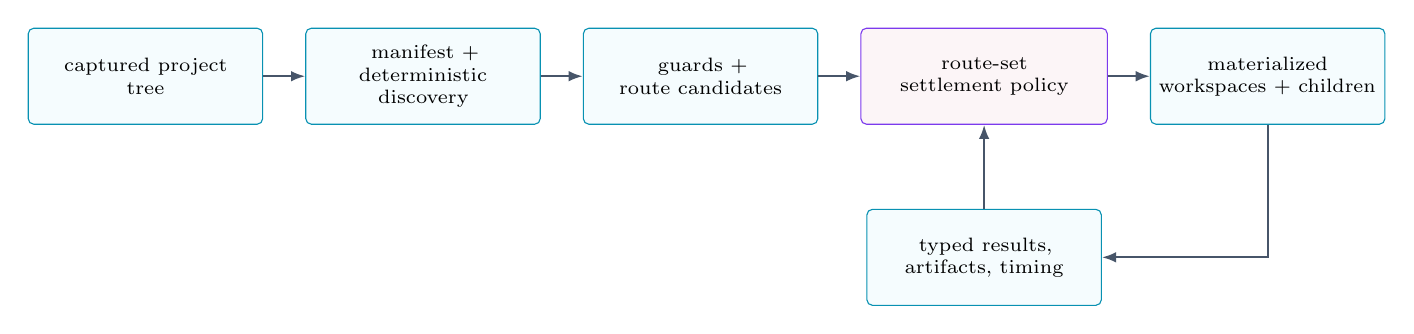
\begin{tikzpicture}[
  node distance=0.21in,
  n/.style={draw=OCyan,rounded corners=2pt,fill=cyan!4,
    text width=1.08in,minimum height=0.48in,align=center,font=\scriptsize},
  p/.style={draw=OPurple,rounded corners=2pt,fill=purple!4,
    text width=1.14in,minimum height=0.48in,align=center,font=\scriptsize},
  a/.style={-{Latex[length=1.8mm]},thick,color=OSlate}
]
  \node[n] (tree) {captured project\\tree};
  \node[n,right=of tree] (discover) {manifest +\\deterministic discovery};
  \node[n,right=of discover] (eligible) {guards +\\route candidates};
  \node[p,right=of eligible] (policy) {route-set\\settlement policy};
  \node[n,right=of policy] (run) {materialized\\workspaces + children};
  \node[n,below=0.42in of policy] (result) {typed results,\\artifacts, timing};
  \foreach \x/\y in {tree/discover,discover/eligible,eligible/policy,policy/run}
    {\draw[a] (\x) -- (\y);}
  \draw[a] (run) |- (result);
  \draw[a] (result.north) -- (policy.south);
\end{tikzpicture}
\caption{Project capture and policy settlement. A route set observes concrete
results until its policy can settle, cancel, compare, or rank candidates.}
\label{fig:project-route-loop}
\end{figure}

The nine public selectors encode distinct settlement algorithms.
\texttt{explicit} chooses a named route; \texttt{default} chooses the declared
default; \texttt{fallback} tries routes sequentially in descending priority
order; \texttt{any\_success} tries declaration order; \texttt{race\_success}
settles on the first success; \texttt{race\_settle} settles on the first
completion; \texttt{all} returns every sequential result, including nonzero
exits; \texttt{verify\_equivalent} runs alternatives concurrently, requires
success, and compares structured results; and
\texttt{benchmark\_and\_select} retains every parallel result while placing
the fastest success last as the effective selection. Route sets are declared
explicitly in the project manifest. A route's \texttt{provides} metadata
describes capability publication and remains independent of route-set
membership.

The tracked \path{tests/fixtures/project_hgraph/olang.project.toml} supplies a
compact authoring example. Its \texttt{main} route set chooses
\texttt{verify\_equivalent} over \texttt{impl-a} and \texttt{impl-b}; both
alternatives depend on \texttt{prepare}. The compiler graph in
Section~\ref{sec:linked-project-dot} shows the resulting isolated branches,
comparison operation, and final selection directly.

\begin{lstlisting}[style=plaincode]
./target/release/o-link tests/fixtures/project_hgraph --project \
  -o output/current-master/o-linked-project.O
./target/release/olangc output/current-master/o-linked-project.O \
  --target ir --route main --shim-dir backends
./target/release/olangc output/current-master/o-linked-project.O \
  --target dot --route main --shim-dir backends
\end{lstlisting}

\subsection{Unlinking}

\texttt{o-unlink} restores both embedded project bundles and literal linked
documents. Project restoration validates relative paths, ancestor symlinks,
and in-root symlink targets before writing. Literal restoration decodes the
escaped file boundaries and rejects absolute paths and parent traversal.
\src{src/bin/ounlink.rs}{49--148}

\section{Toolchain and implementation editions}
\label{sec:toolchain}

\subsection{Public binaries}

The root Cargo package declares fourteen binaries.

\begin{longtable}{P{0.32\textwidth} P{0.60\textwidth}}
\toprule
\textbf{Binary} & \textbf{Implemented role} \\
\midrule
\endhead
\texttt{O} &
Hosted interpreter, REPL, executor selection, compatibility backend grants,
and hidden backend worker mode. \\
\texttt{o-cli} &
Compiled lowercase intent front door for run, plan, explain, inspect, and
durable run records. \\
\texttt{olangc} &
Hosted packaging/compiler front end: binary, WASM, script, IR, and DOT. \\
\texttt{ocorec} &
\ocore{} compiler: AST, HIR, MIR, assembly, or relocatable object. \\
\texttt{o-link} / \texttt{o-unlink} &
Literal linking and safe project bundle lift/restoration. \\
\texttt{o-notebook} &
Feature-gated local notebook server with per-process O scope and typed result
rendering. \\
\texttt{ogit} &
Bounded semantic-receipt and policy-aware diff demonstration. \\
\texttt{o-live-host} &
Hosted Live-World lifecycle oracle. \\
\texttt{o-node} / \texttt{octl} &
Hosted node service, discovery, reciprocal pairing, paired TLS operation, and
node-control client. \\
\texttt{o-registry} / \texttt{o-info} &
Registry V1 event operations and Information-root inspection. \\
\path{ocore-kernel-world-record} &
Verify a strict package/payload pair and encode its deterministic native
admission record. \\
\bottomrule
\end{longtable}

\src{Cargo.toml}{20--76}

\subsection{What olangc targets mean}

\begin{longtable}{P{0.16\textwidth} P{0.47\textwidth} P{0.29\textwidth}}
\toprule
\textbf{Target} & \textbf{Implementation} & \textbf{Execution model} \\
\midrule
\endhead
\texttt{binary} &
Generates a temporary Cargo project containing embedded source, runtime
modules, shims, and a lockfile; builds a host executable. &
The generated executable embeds the hosted runtime, reparses its source at
startup, and evaluates through the ordinary graph path. \\
\texttt{wasm} &
Uses the generated-runtime path for \texttt{wasm32-wasip1}. &
Produces a WASI module containing the generated hosted runtime and embedded
program. \\
\texttt{script} &
Parses and invokes the normal evaluator inside \texttt{olangc}. &
This is the direct compiler-driver entry into hosted graph evaluation. \\
\texttt{ir} &
Prints \oir{}, the execution plan, and \hgraph{}. &
It exposes structural lowering, frozen interfaces, dependencies, and resource
state in one inspection stream. \\
\texttt{dot} &
Solves and renders directed graph operation ports. &
It visualizes executable operations and the value/resource ports connecting
them. \\
\bottomrule
\end{longtable}

\src{src/bin/olangc.rs}{130--258}
\src{src/bin/olangc.rs}{923--1473}
\src{src/bin/olangc.rs}{1910--2365}

Project inputs compile through binary, WASM, and script targets. The generated
project runtime restores the captured tree and executes its selected
subprocess route, carrying whole-project structure into the packaged artifact.
Project directories and lifted bundles also enter the IR and DOT targets,
which build the exact logical Project HGraph for the selected route or route
set. A generated project WASI module contains the project runtime; its route
operations use the process facilities supplied by the execution substrate.

\subsection{Reference implementations}

The Rust edition is authoritative and implements the full hosted graph,
project, Live-World, and \ocore{} surfaces. The Python edition identifies
itself as the original/reference implementation at version 0.4.0. It has a
compact recursive evaluator and uses environment 0 as persistent by default.
The C17 edition supplies a portable hosted interpreter and hosted AOT path.
Together, these editions provide independently executable semantic references
around the authoritative Rust graph runtime.
\src{o_lang/README.md}{1--14}
\src{o_lang/__init__.py}{31--40}
\src{o_lang/evaluator.py}{1--182}
\src{c_cpp/README.md}{1--133}

\begin{longtable}{P{0.18\textwidth} P{0.34\textwidth} P{0.40\textwidth}}
\toprule
\textbf{Edition} & \textbf{Parser-visible evaluator registry} &
\textbf{Implementation surface} \\
\midrule
\endhead
Rust 0.4.0 Unreleased &
30 canonical tags and six aliases listed in Section~\ref{sec:backends}. &
OIR, plans, HGraph, both schedulers, projects, native and WASI generation,
REPL, notebook, O-Git, Live-World, KernelWorld records, and \ocore{}. \\
Python 0.4.0 &
\texttt{python}, \texttt{markdown}, \texttt{html}, \texttt{latex},
\texttt{text}, \texttt{O}, \texttt{quote}, \texttt{nix},
\texttt{nix\_store}, \texttt{nixos\_test}; aliases \texttt{py},
\texttt{md}, \texttt{tex}, \texttt{plain}, \texttt{o}. &
Direct execution, AST dump, text/HTML/Markdown/LaTeX/JSON projections,
file output, the typed root API below, parser tests, and evaluator tests. \\
C17 interpreter &
\texttt{O}, \texttt{python}, \texttt{html}, \texttt{latex},
\texttt{markdown}, \texttt{bash}, \texttt{shell}, \texttt{rust},
\texttt{racket}, \texttt{nix}, \texttt{nix\_expr},
\texttt{nix\_store}, \texttt{nixos\_test}, \texttt{quote}. &
Portable hosted parsing, evaluation, embedding headers, and backend-process
execution through the C17 test corpus. \\
C17 AOT &
The interpreter registry plus \texttt{text}. &
Generated C, host compilation, hello execution, and meta-evaluation. \\
\bottomrule
\end{longtable}

The Python package root exposes its complete small embedding vocabulary:

\begin{longtable}{P{0.20\textwidth} P{0.72\textwidth}}
\toprule
\textbf{API family} & \textbf{Public names} \\
\midrule
\endhead
Parse and evaluate & \texttt{run}, \texttt{parse},
\texttt{evaluate\_document}, \texttt{EvalContext}, \texttt{pretty}. \\
Syntax tree & \texttt{Document}, \texttt{ExpressionNode}, \texttt{TextPart}. \\
Values & \texttt{OValue}, \texttt{ONull}, \texttt{OBool}, \texttt{OInt},
\texttt{OFloat}, \texttt{OStr}, \texttt{OHtml}, \texttt{OStorePath},
\texttt{OList}, \texttt{OMap}, \texttt{OScope}, \texttt{OBlob},
\texttt{OExpr}. \\
Conversion and rendering & \texttt{from\_python}, \texttt{to\_python},
\texttt{render\_plain}, \texttt{to\_json\_str}. \\
\bottomrule
\end{longtable}
\src{o_lang/__init__.py}{12--38}

The C17 edition publishes six headers as an embedding ABI:

\begin{longtable}{P{0.17\textwidth} P{0.75\textwidth}}
\toprule
\textbf{Header} & \textbf{Public integration surface} \\
\midrule
\endhead
\texttt{value.h} & Tagged OValue union, constructors, reference counting,
maps, content identity, JSON, length-prefixed CBOR frames, SHA-256, and base64. \\
\texttt{parser.h} & AST storage, registered-language sets, parser lifecycle,
tree destruction, and source reconstruction. \\
\texttt{eval.h} & Eager, lazy, and autonomous policy; evaluator lifecycle,
document and source evaluation, rendering, and shim lookup. \\
\texttt{process.h} & Backend processes, reentrant evaluation steps, and the
persistent $(language, environment)$ process registry. \\
\texttt{scheduler.h} & Disk cache, configurable autonomous scheduler, batch
callbacks, and transitive-request collection. \\
\texttt{nix\_ops.h} & Typed instantiate, realise, activate or dry-activate,
and current-system transitions. \\
\bottomrule
\end{longtable}
\src{c_cpp/include/value.h}{13--222}
\src{c_cpp/include/parser.h}{23--114}
\src{c_cpp/include/eval.h}{16--54}
\src{c_cpp/include/process.h}{13--73}
\src{c_cpp/include/scheduler.h}{13--49}
\src{c_cpp/include/nix_ops.h}{10--21}

\subsection{REPL and notebook state}

The interactive surfaces expose two deliberate state lifetimes. The REPL
retains O lexical bindings and evaluator-owned backend actors across entries.
Its \texttt{:r} command replaces the O lexical scope while leaving persistent
actor processes available. The notebook binds \texttt{127.0.0.1:8888} and
places one \texttt{Session} behind a process-wide mutex. Every browser client
therefore observes the same O scope and evaluator registry. A POST to
\texttt{/reset} replaces that complete session, clearing both lexical bindings
and actor state. GET \texttt{/} serves the embedded interface, while POST
\texttt{/eval} returns tagged null, text, HTML, or image output.

\begin{figure}[htbp]
\centering
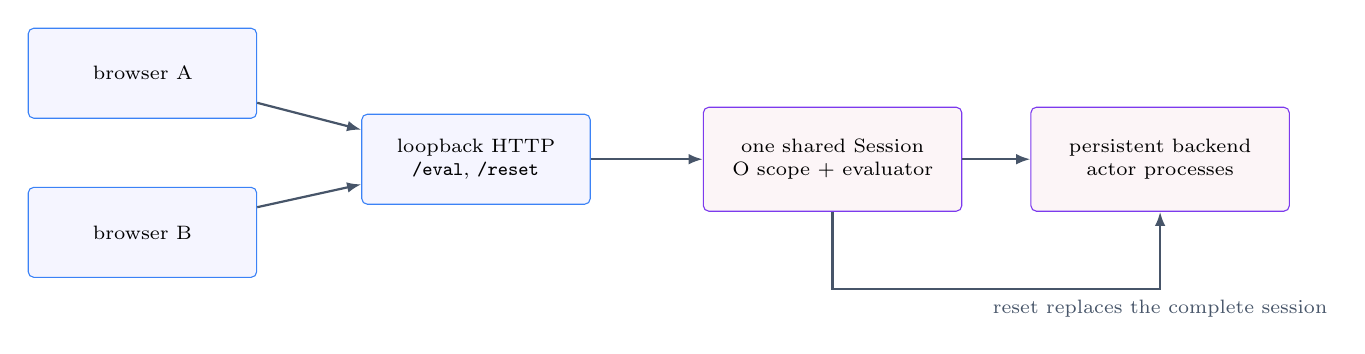
\begin{tikzpicture}[
  node distance=0.34in,
  c/.style={draw=OBlue,rounded corners=2pt,fill=blue!4,
    text width=1.05in,minimum height=0.45in,align=center,font=\scriptsize},
  s/.style={draw=OPurple,rounded corners=2pt,fill=purple!4,
    text width=1.20in,minimum height=0.52in,align=center,font=\scriptsize},
  a/.style={-{Latex[length=1.8mm]},thick,color=OSlate}
]
  \node[c] (b1) {browser A};
  \node[c,below=of b1] (b2) {browser B};
  \node[c,right=0.52in of b1,yshift=-0.43in] (http) {loopback HTTP\\\texttt{/eval}, \texttt{/reset}};
  \node[s,right=0.56in of http] (session) {one shared Session\\O scope + evaluator};
  \node[s,right=of session] (actors) {persistent backend\\actor processes};
  \draw[a] (b1) -- (http);
  \draw[a] (b2) -- (http);
  \draw[a] (http) -- (session);
  \draw[a] (session) -- (actors);
  \draw[a] (session) |- ++(0,-0.65in) -| node[below,font=\scriptsize]
    {reset replaces the complete session} (actors);
\end{tikzpicture}
\caption{The local notebook has one process-wide interactive state. Cell
evaluation preserves both O bindings and backend actors; reset creates a new
scope and evaluator together.}
\label{fig:notebook-state}
\end{figure}

\subsection{O-Git}

O-Git demonstrates semantic receipts and policy-aware diffs. A receipt records
source and target paths, group declarations, output, and qualitative
properties classified as preserved, lowered, erased, or assumed. The command
turns semantic transformation choices into a machine-readable artifact that
can be compared alongside ordinary repository history.
\par\src{src/bin/ogit.rs}{96--183}\quad
\src{src/bin/ogit.rs}{523--576}

The checked-in \path{examples/group_pipeline/main.O} and
\path{main.eager.O} are receipt inputs that expose a lazy-to-eager policy
change. O-Git lowers and executes its generated C target, then records the
semantic transformation. Direct hosted O evaluation encounters their
unforced \texttt{\{defer\}} splice, so an executable hosted variant would place
\texttt{now(...)} at that force point. This is the exact semantic distinction
the receipt is designed to preserve.

\section{O-core: the native language}
\label{sec:ocore}

\subsection{Language surface}

Every \texttt{.oc} unit begins with a module declaration. The lexer and AST
cover imports and visibility; functions, unsafe and extern declarations;
structures, enums, statics, and constants; conditional and loop control;
arrays and aggregate construction; direct calls; field and index access;
casts; volatile operations; and inline assembly.
\src{crates/ostadix-api/src/ocore/lexer.rs}{9--88}
\src{crates/ostadix-api/src/ocore/parser.rs}{23--107}
\src{crates/ostadix-api/src/ocore/ast.rs}{5--285}

Supported foreign interfaces include \texttt{extern "sysv64"},
\texttt{extern "C"}, and \texttt{extern "ocore"}. A \texttt{let} requires an
initializer, assignment is right-associative, and binary precedence is
encoded in the parser. Inline assembly has explicit syntax and operands.
\src{crates/ostadix-api/src/ocore/parser.rs}{335--755}

The checked-in minimal unit shows the source spelling that was compiled through
AST, HIR, MIR, assembly, and reproducible ELF object output in this release:

\begin{lstlisting}[style=plaincode]
module examples::minimal;

@export
pub fn add(left: u64, right: u64) -> u64 {
    return left + right;
}
\end{lstlisting}
\src{ocore/examples/minimal.oc}{1--6}

The module declaration names the unit, \texttt{@export} fixes external
visibility, \texttt{pub} admits cross-module lookup, the signature fixes every
machine type, and the explicit return becomes typed SSA before x86-64 lowering.
Structures, enums, imports, statics, constants, extern declarations, unsafe
blocks, volatile and atomic intrinsics, and \texttt{asm!} use the same direct
item-and-expression grammar across the current 132-file O-core source corpus:
77 runtime files, 46 kernel files, eight World files, and one example.
\src{docs/OCORE.md}{36--75}
\src{docs/OCORE.md}{140--190}

\subsection{Static semantics}

Type checking proceeds in dependency-aware passes:

\begin{center}
module scopes $\rightarrow$ type names $\rightarrow$ layouts
$\rightarrow$ signatures $\rightarrow$ constants/statics
$\rightarrow$ bodies.
\end{center}

Unsafe operations require an explicit unsafe context. Attributes are
whitelisted; unknown ones are rejected. Interrupt and naked functions,
aggregate calls, and floating-point ABI crossings receive explicit defensive
checks. \src{crates/ostadix-api/src/ocore/typeck.rs}{16--59}
\src{crates/ostadix-api/src/ocore/typeck.rs}{1881--2038}

\subsubsection{Types, aggregates, and layout}

The scalar set is \texttt{bool}; unsigned \texttt{u8}, \texttt{u16},
\texttt{u32}, \texttt{u64}, and \texttt{usize}; signed \texttt{i8},
\texttt{i16}, \texttt{i32}, \texttt{i64}, and \texttt{isize};
\texttt{f32}, \texttt{f64}, \texttt{void}, and \texttt{never}. Compound types
are fixed arrays \texttt{[T; N]}, immutable and mutable raw pointers,
declaration-ordered structures, tagged enums, and function-pointer types.
Structures support construction, fields, locals, statics, and aggregate copy.
Arrays support literals, repetition, indexing, locals, statics, and explicit
address operations. Enum layout combines the smallest adequate
\texttt{u8}/\texttt{u16}/\texttt{u32} tag with an aligned payload region.

\begin{center}
\begin{tabular}{lrr}
\toprule
\textbf{Type class} & \textbf{Size (bytes)} & \textbf{Alignment} \\
\midrule
\texttt{bool}, \texttt{u8}, \texttt{i8} & 1 & 1 \\
\texttt{u16}, \texttt{i16} & 2 & 2 \\
\texttt{u32}, \texttt{i32}, \texttt{f32} & 4 & 4 \\
\texttt{u64}, \texttt{i64}, \texttt{usize}, \texttt{isize},
\texttt{f64}, pointers & 8 & 8 \\
\texttt{void}, \texttt{never} & 0 & 1 \\
\bottomrule
\end{tabular}
\end{center}

Natural padding preserves declaration order. \texttt{@packed} selects
alignment 1 and removes inter-field padding; \texttt{@align(N)} raises
alignment to a power of two. System V scalar calls use RDI, RSI, RDX, RCX, R8,
and R9, followed by stack arguments, with RAX as the scalar result and
16-byte call alignment. \texttt{@interrupt} functions return with
\texttt{iretq}. \src{docs/OCORE.md}{95--193}

\subsubsection{Name, conversion, storage, and call semantics}

One \texttt{ocorec} invocation forms a compilation unit from one or more source
files, each with a unique module name. Unqualified lookup proceeds through
local bindings, current-module items, explicit imports, and predeclared
intrinsics. Cross-module functions receive deterministic mangled symbols;
\texttt{@export} and \texttt{@no\_mangle} state the external symbol contract.

An unsuffixed integer literal inherits an expected integer type. Every other
numeric or pointer conversion is written with \texttt{as}. Raw pointer
arithmetic and dereference, pointer/integer conversion, mutable-static access,
inline assembly, and privileged intrinsics require an explicit unsafe context.
Values use deterministic destruction-free storage. Stack objects, statics,
raw pointers, and explicitly linked runtime allocators state every storage
lifetime at the freestanding boundary. Heap allocation occurs through an
explicitly linked runtime allocator, keeping lifetime management explicit.

Direct scalar calls lower through the selected ABI, and function-pointer types
carry call signatures through parsing and type checking. Aggregate parameters
and aggregate returns are rejected across direct and extern call boundaries;
authors pass pointers explicitly. Floating-point values have fixed storage
layouts and bit-preserving transport. \src{docs/OCORE.md}{36--134}
\src{crates/ostadix-api/src/ocore/typeck.rs}{2028--2038}

\subsubsection{Machine operations and linkage}

The volatile/atomic surface is \path{volatile_load},
\path{volatile_store}, \path{atomic_load}, \path{atomic_store},
\path{atomic_exchange}, \path{atomic_compare_exchange}, and
\path{atomic_fetch_add}. Orders are \texttt{relaxed}, \texttt{acquire},
\texttt{release}, \texttt{acq\_rel}, and \texttt{seq\_cst}; the type checker
validates operation width, mutability, and legal order combinations before
code generation. Hardware intrinsics cover byte/word/dword port input and
output, interrupt enable/disable, halt, page invalidation, \texttt{syscall0}
through \texttt{syscall6}, and Intel-syntax \texttt{asm!} with explicit
register operands and memory/stack options.

The linkage attributes are \texttt{@export}, \texttt{@no\_mangle},
\texttt{@link\_section("name")}, \texttt{@align(N)}, \texttt{@used},
\texttt{@packed}, \texttt{@interrupt}, and \texttt{@naked}. Together they let
O-core source state symbol visibility, exact symbol names, ELF placement,
retention, layout, and entry/exit discipline directly. \texttt{@unsafe\_linkage}
explicitly admits a writable
static placed in an executable section. \src{docs/OCORE.md}{170--192}

\subsection{Compiler pipeline}

\begin{figure}[htbp]
\centering
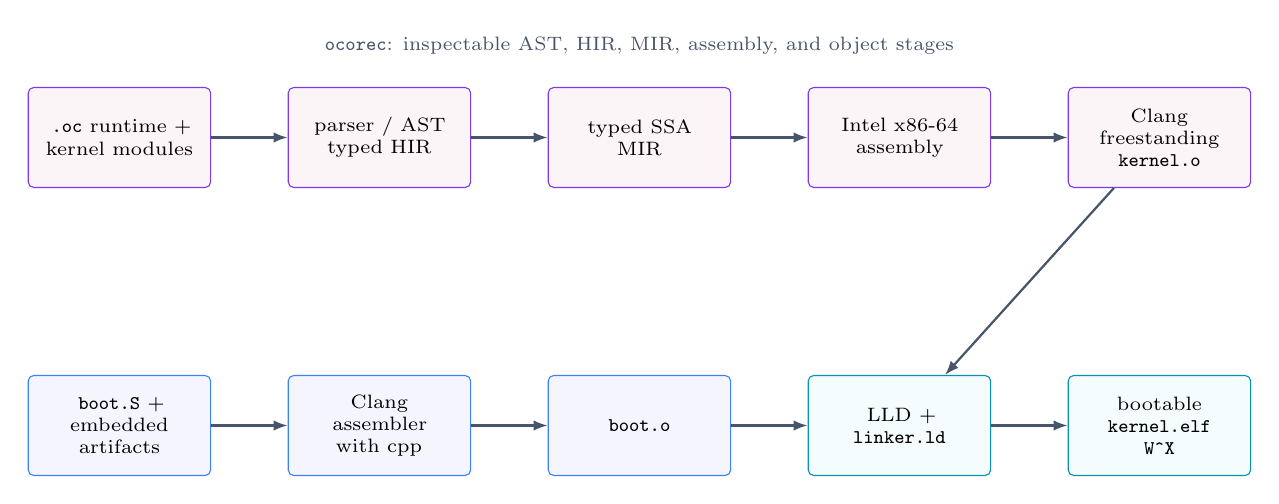
\begin{tikzpicture}[
  x=1in,y=1in,
  every node/.style={font=\scriptsize},
  compiler/.style={draw=OPurple,rounded corners=2pt,fill=purple!4,
    minimum height=0.50in,text width=0.82in,align=center},
  boot/.style={draw=OBlue,rounded corners=2pt,fill=blue!4,
    minimum height=0.50in,text width=0.82in,align=center},
  link/.style={draw=OCyan,rounded corners=2pt,fill=cyan!4,
    minimum height=0.50in,text width=0.82in,align=center},
  a/.style={-{Latex[length=1.8mm]},thick,color=OSlate}
]
  \node[compiler] (src) at (0,0.72) {\texttt{.oc} runtime +\\kernel modules};
  \node[compiler] (front) at (1.30,0.72) {parser / AST\\typed HIR};
  \node[compiler] (mir) at (2.60,0.72) {typed SSA\\MIR};
  \node[compiler] (asm) at (3.90,0.72) {Intel x86-64\\assembly};
  \node[compiler] (obj) at (5.20,0.72) {Clang\\freestanding\\\texttt{kernel.o}};

  \node[boot] (bootsrc) at (0,-0.72) {\texttt{boot.S} +\\embedded artifacts};
  \node[boot] (bootasm) at (1.30,-0.72) {Clang\\assembler with cpp};
  \node[boot] (bootobj) at (2.60,-0.72) {\texttt{boot.o}};
  \node[link] (lld) at (3.90,-0.72) {LLD +\\\texttt{linker.ld}};
  \node[link] (elf) at (5.20,-0.72) {bootable\\\texttt{kernel.elf}\\
    \texttt{W\textasciicircum X}};

  \foreach \a/\b in {src/front,front/mir,mir/asm,asm/obj,bootsrc/bootasm,bootasm/bootobj,bootobj/lld,lld/elf}
    {\draw[a] (\a) -- (\b);}
  \draw[a] (obj) -- (lld);
  \node[font=\scriptsize\color{OSlate}] at (2.60,1.18)
    {\texttt{ocorec}: inspectable AST, HIR, MIR, assembly, and object stages};
\end{tikzpicture}
\caption{The native build has two feeders. \texttt{ocorec} compiles O-core
modules into a freestanding object; boot assembly, embedded mode artifacts,
and the linker script complete the Multiboot2/Xen-PVH kernel image.}
\label{fig:ocore-kernel-build}
\end{figure}

MIR is typed SSA, while mutable locals and statics remain explicit memory
places. The code generator emits Intel-syntax x86-64 and gives every local
and SSA value stack storage. Clang assembles with
\texttt{x86\_64-unknown-none-elf}, freestanding settings, and the stack
protector disabled. \src{crates/ostadix-api/src/ocore/mir.rs}{1--173}
\src{crates/ostadix-api/src/ocore/codegen.rs}{1--20}
\src{crates/ostadix-api/src/ocore/codegen.rs}{162--317}
\src{crates/ostadix-api/src/ocore/driver.rs}{126--183}

\subsection{Current compiler profile}

The current backend targets freestanding x86-64 under the System V AMD64 ABI.
Its lowering uses stack storage for locals and SSA values, direct calls,
explicit aggregate layouts, integer and pointer operations, volatile memory,
and inline assembly. Programs manage memory through statics, stack objects,
pointers, and explicitly linked runtime facilities. \src{docs/OCORE.md}{351--365}

\begin{claimbox}[Native compiler substance]
\ocore{} has a complete parser, layout-aware type checker, typed SSA MIR,
defensive ABI rules, deterministic x86-64 assembly, and reproducible ELF
object tests. That pipeline makes the language executable at the machine
boundary and provides the source language for the Ostadix freestanding runtime
and kernel.
\end{claimbox}

\section{Kernel, capabilities, and native execution}
\label{sec:kernel}

\subsection{Freestanding kernel substrate}

The kernel build links a complete set of \texttt{.oc} runtime modules with
boot assembly and a linker script. It uses Rust/Cargo \texttt{ocorec} on the
host, Clang for assembly, and LLD for ELF linking. The image contains
Multiboot2 and Xen PVH metadata, \texttt{W\textasciicircum X} program headers,
fixed user RX and RW-NX
regions, guard-page checks, and fail-closed initialization of memory,
process/domain, scheduler, capability, mapping, and IPC state.
\src{ocore/kernel/build.sh}{358--529}
\src{ocore/kernel/linker.ld}{1--105}
\src{ocore/kernel/main.oc}{180--496}

\subsection{Native capability model}

Native handles encode
\[
(\textit{generation} \ll 32)\ |\ \textit{slot},
\]
while CSpace identity remains kernel-private. Validation checks the current
CSpace, slot, occupancy, generation, object kind, and rights. Reservation
and close are explicit transactions; generation exhaustion retires a slot.
Memory-view and delegated-resource authority is deliberately nontransferable.
\src{ocore/runtime/x86_64/capability.oc}{21--69}
\src{ocore/runtime/x86_64/capability.oc}{294--394}
\src{ocore/runtime/x86_64/capability.oc}{520--543}
\src{ocore/runtime/x86_64/capability.oc}{752--880}

The kernel syscall contract fixes authority checks to seventeen numbered
operations. A caller supplies generated handles; the dispatcher derives the
current PCB and CSpace, validates object kind, generation, and rights, and then
performs the operation.

\begin{longtable}{r P{0.28\textwidth} P{0.56\textwidth}}
\toprule
\textbf{No.} & \textbf{Operation} & \textbf{Contract} \\
\midrule
\endhead
0 & \texttt{debug\_write} & Capability-gated bounded copy from readable user memory. \\
1 & \texttt{cap\_close} & Close one generation-tagged CSpace entry. \\
2 & \texttt{cap\_copy} & Prepare an attenuation-only transfer ticket to an authorized endpoint's receiver. \\
3 & \texttt{page\_alloc} & Allocate a typed page object and return a kernel-selected capability. \\
4 & \texttt{yield} & Record or perform a cooperative scheduler transition. \\
5 & \texttt{ticks} & Return the diagnostic timer count. \\
6 & \texttt{exit} & Enter the configured trusted lifecycle continuation. \\
7 & \texttt{sleep} & Block until a scheduler-managed tick deadline. \\
8 & \texttt{endpoint\_create} & Create and return a generation-safe endpoint. \\
9 & \texttt{endpoint\_send} & Send two words plus an optional transfer ticket. \\
10 & \texttt{endpoint\_receive} & Receive one bounded 32-byte message. \\
11 & \texttt{endpoint\_cancel} & Cancel by endpoint and correlation identity. \\
12 & \texttt{serial\_read} & Read one nonblocking byte through the exact control capability. \\
13 & \texttt{control\_submit} & Submit one checked command of at most 192 bytes. \\
14 & \texttt{personality\_call} & Invoke the M6A scalar route with a deadline. \\
15 & \texttt{personality\_reply} & Complete an exact M6A request through a reply capability. \\
16 & \texttt{personality\_supervise} & Apply an M6A policy action to an exact generation and subject. \\
\bottomrule
\end{longtable}

The message path uses fault-aware bounded copy, FIFO endpoint queues, real TCB
block/wake epochs, request correlation, lifecycle cancellation, and exact
attenuation. The scalar personality calls use distinct call, reply, and
supervision capability kinds, so operation role is carried by authority rather
than a caller-provided mode bit. \src{docs/OCORE.md}{205--284}
\src{docs/OCORE.md}{442--496}

\begin{figure}[H]
\centering
\resizebox{0.98\textwidth}{!}{%
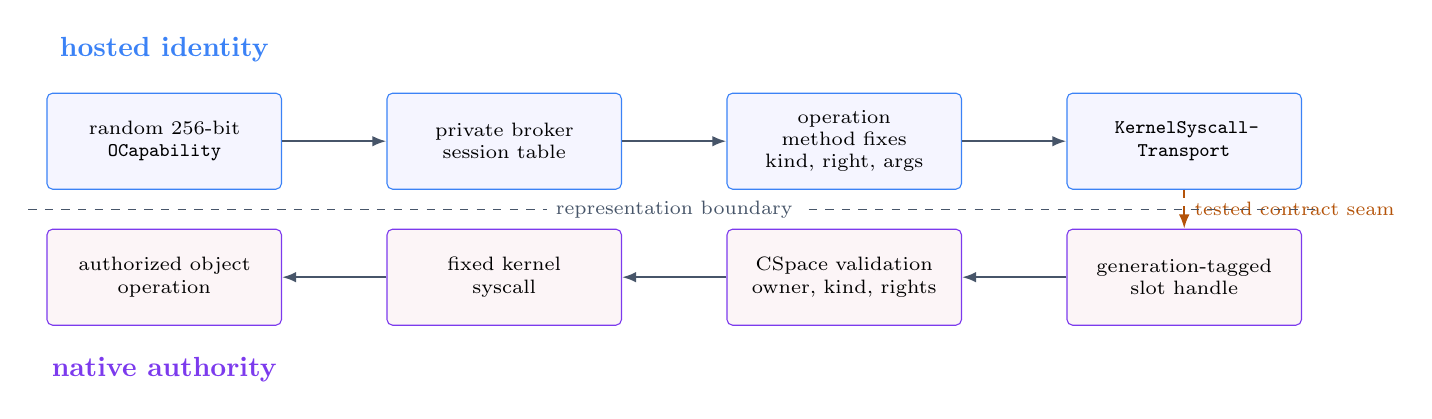
\begin{tikzpicture}[
  x=1in,y=1in,
  every node/.style={font=\scriptsize},
  hosted/.style={draw=OBlue,rounded corners=2pt,fill=blue!4,
    text width=1.08in,minimum height=0.48in,align=center},
  native/.style={draw=OPurple,rounded corners=2pt,fill=purple!4,
    text width=1.08in,minimum height=0.48in,align=center},
  arr/.style={-{Latex[length=1.8mm]},thick,color=OSlate},
  seam/.style={-{Latex[length=1.8mm]},thick,dashed,color=OAmber}
]
  \node[font=\bfseries\color{OBlue}] at (0,0.80) {hosted identity};
  \node[hosted] (bearer) at (0,0.34) {random 256-bit\\\texttt{OCapability}};
  \node[hosted] (broker) at (1.70,0.34) {private broker\\session table};
  \node[hosted] (method) at (3.40,0.34) {operation method fixes\\kind, right, args};
  \node[hosted] (transport) at (5.10,0.34) {\texttt{KernelSyscall-}\\\texttt{Transport}};

  \node[font=\bfseries\color{OPurple}] at (0,-0.80) {native authority};
  \node[native] (result) at (0,-0.34) {authorized object\\operation};
  \node[native] (syscall) at (1.70,-0.34) {fixed kernel\\syscall};
  \node[native] (validate) at (3.40,-0.34) {CSpace validation\\owner, kind, rights};
  \node[native] (handle) at (5.10,-0.34) {generation-tagged\\slot handle};

  \draw[arr] (bearer) -- (broker);
  \draw[arr] (broker) -- (method);
  \draw[arr] (method) -- (transport);
  \draw[seam] (transport) -- node[right,font=\scriptsize\color{OAmber}]
    {tested contract seam} (handle);
  \draw[arr] (handle) -- (validate);
  \draw[arr] (validate) -- (syscall);
  \draw[arr] (syscall) -- (result);
  \draw[OSlate,dashed] (-0.68,0) -- (5.78,0);
  \node[fill=white,font=\scriptsize\color{OSlate}] at (2.55,0)
    {representation boundary};
\end{tikzpicture}
}
\caption{The bridge preserves hosted bearer identity and kernel-owned native
authority. Operation-specific contracts cross the transport seam; CSpace
validation resolves generation, object kind, and rights before execution. A
private session table owns bearer-to-handle bindings, while recording and
failure transports verify the exact calls.}
\label{fig:capability-bridge}
\end{figure}

\par\src{crates/ostadix-api/src/ocore/capability_bridge.rs}{1--159}

\clearpage
\section{Live-World and KernelWorld}
\label{sec:world}

\begin{figure}[H]
\centering
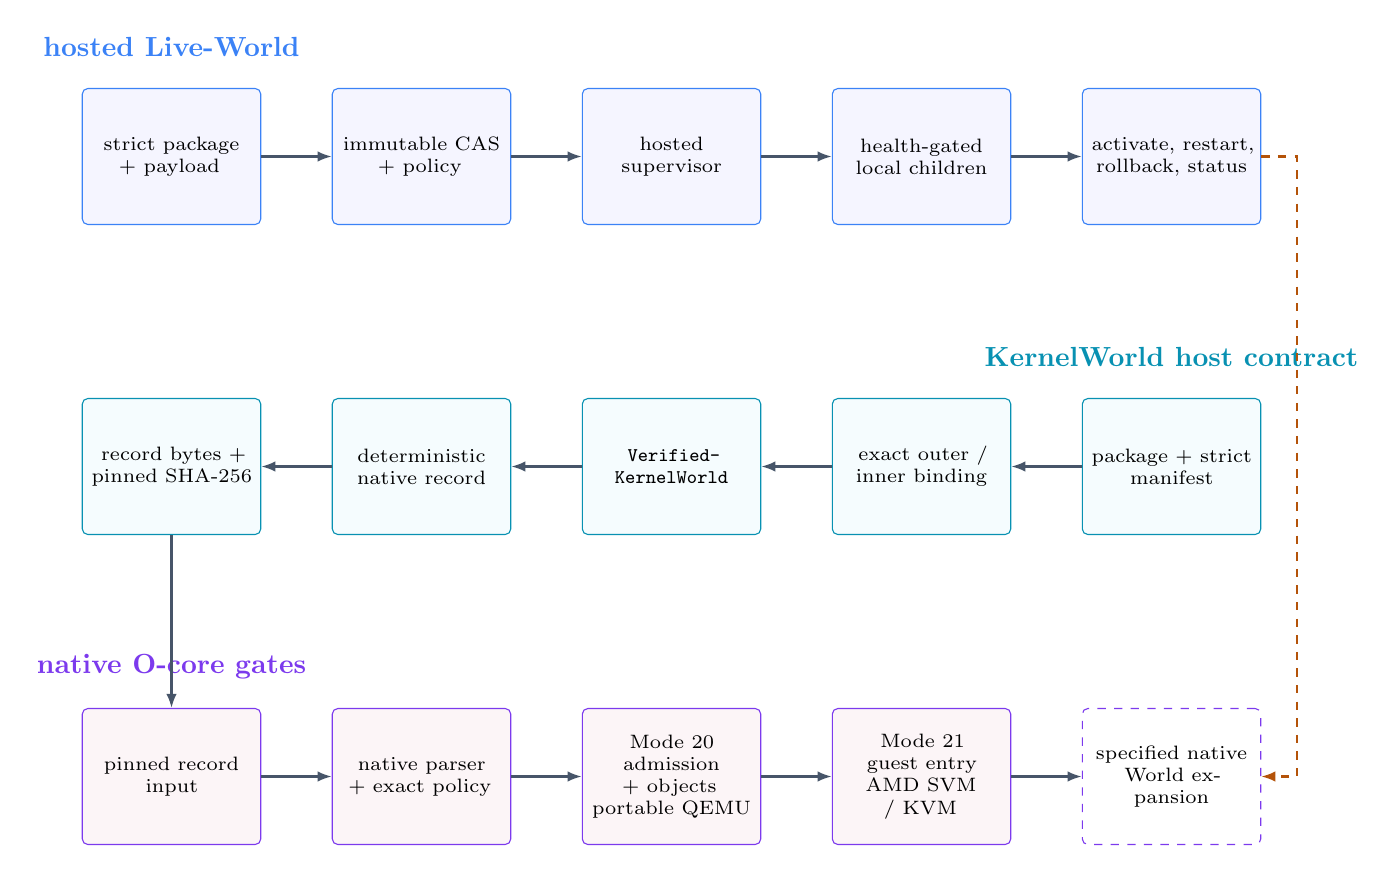
\begin{tikzpicture}[
  x=1in,y=1in,
  every node/.style={font=\scriptsize},
  hosted/.style={draw=OBlue,rounded corners=2pt,fill=blue!4,
    text width=0.80in,minimum height=0.68in,align=center},
  contract/.style={draw=OCyan,rounded corners=2pt,fill=cyan!4,
    text width=0.80in,minimum height=0.68in,align=center},
  native/.style={draw=OPurple,rounded corners=2pt,fill=purple!4,
    text width=0.80in,minimum height=0.68in,align=center},
  future/.style={native,dashed,fill=white},
  arr/.style={-{Latex[length=1.8mm]},thick,color=OSlate},
  compare/.style={-{Latex[length=1.8mm]},dashed,color=OAmber,thick}
]
  \node[font=\bfseries\color{OBlue}] at (0,2.10) {hosted Live-World};
  \node[hosted] (hpkg) at (0,1.55) {strict package\\+ payload};
  \node[hosted] (cas) at (1.25,1.55) {immutable CAS\\+ policy};
  \node[hosted] (supervisor) at (2.50,1.55) {hosted\\supervisor};
  \node[hosted] (children) at (3.75,1.55) {health-gated\\local children};
  \node[hosted] (lifeops) at (5.00,1.55) {activate, restart,\\rollback, status};
  \foreach \a/\b in {hpkg/cas,cas/supervisor,supervisor/children,children/lifeops}
    {\draw[arr] (\a) -- (\b);}

  \node[font=\bfseries\color{OCyan}] at (5.00,0.55) {KernelWorld host contract};
  \node[contract] (manifest) at (5.00,0) {package + strict\\manifest};
  \node[contract] (binding) at (3.75,0) {exact outer /\\inner binding};
  \node[contract] (verified) at (2.50,0) {\texttt{Verified-}\\\texttt{KernelWorld}};
  \node[contract] (record) at (1.25,0) {deterministic\\native record};
  \node[contract] (pinned) at (0,0) {record bytes +\\pinned SHA-256};
  \foreach \a/\b in {manifest/binding,binding/verified,verified/record,record/pinned}
    {\draw[arr] (\a) -- (\b);}

  \node[font=\bfseries\color{OPurple}] at (0,-1.00) {native O-core gates};
  \node[native] (nativebytes) at (0,-1.55) {pinned record\\input};
  \node[native] (parser) at (1.25,-1.55) {native parser\\+ exact policy};
  \node[native] (mode20) at (2.50,-1.55) {Mode 20\\admission + objects\\portable QEMU};
  \node[native] (mode21) at (3.75,-1.55) {Mode 21 guest entry\\AMD SVM / KVM};
  \node[future] (future) at (5.00,-1.55) {specified native\\World expansion};
  \foreach \a/\b in {nativebytes/parser,parser/mode20,mode20/mode21,mode21/future}
    {\draw[arr] (\a) -- (\b);}

  \draw[arr] (pinned) -- (nativebytes);
  \draw[compare] (lifeops.east) -- ++(0.18in,0) |- (future.east);
\end{tikzpicture}
\caption{World semantics, host verification, and native execution occupy
separate substrates. The record path is a solid authority chain into native
admission. The dashed path marks differential comparison between hosted
lifecycle behavior and the specified native continuation.}
\label{fig:world-substrates}
\end{figure}

\subsection{Three different layers}

\begin{longtable}{P{0.20\textwidth} P{0.38\textwidth} P{0.34\textwidth}}
\toprule
\textbf{Layer} & \textbf{Implemented substrate} & \textbf{Architectural role} \\
\midrule
\endhead
Hosted Live-World &
Local child processes, immutable content store, strict manifests, policy,
health checks, rollback/restart/reconstruction, and private bearers. &
Executable lifecycle semantics and a differential oracle for native World
stages. \\
Native M5 slice &
Separately loaded x86-64 ELF services and CSpaces under QEMU, a serial control
loop, and generation-based crash/restart behavior. &
Machine-level service isolation, capability routing, crash recovery, and
generation replacement in the M5 execution gate. \\
Target architecture &
Independent unprivileged endpoint-RPC services, durable reconstruction, and a
native build service. &
The specified expansion path from the implemented native service substrate to
a complete World lifecycle. \\
\bottomrule
\end{longtable}

\src{docs/HOSTED_LIVE_REFERENCE.md}{1--99}
\src{docs/LIVE_SYSTEM.md}{3--47}

Hosted advisory locks and revision compare-and-swap serialize lifecycle
transactions over the local immutable content store. Supervisor code
implements generation rotation, bearer issuance, exact live-binding
invocation, restart, and stale-generation denial.
\src{crates/ostadix-api/src/live_system/supervisor.rs}{770--1007}

\subsection{Live-World command and state model}

The public \texttt{o-live-host} surface is a complete local lifecycle. A
package enters an immutable content-addressed store, activation creates a
health-checked service generation, invocation resolves the exact active
binding, composition passes \ovalue{} between worlds, and every mutation
records enough state for reconstruction.

\begin{longtable}{P{0.16\textwidth} P{0.34\textwidth} P{0.42\textwidth}}
\toprule
\textbf{Command} & \textbf{State transition} & \textbf{Resulting state} \\
\midrule
\endhead
\texttt{pack} & Canonical manifest and payload $\rightarrow$ exact package digest. &
Emits the content identity calculated over canonical manifest semantics and
the exact captured payload tree. \\
\texttt{install} & Verified package $\rightarrow$ immutable CAS object. &
Writes the object and strict alias metadata into the content-addressed store. \\
\texttt{activate} & Policy admission + health $\rightarrow$ active generation. &
Publishes a health-checked service generation and its exact policy grants. \\
\texttt{invoke} & Active bearer + ABI + operation $\rightarrow$ tagged result. &
Resolves the exact live binding and returns a bounded tagged \ovalue{}. \\
\texttt{compose} & Invoke chain $\rightarrow$ \ovalue{} transfer between worlds. &
Passes each typed result into the next declared service operation. \\
\texttt{upgrade} & Candidate health + generation rotation $\rightarrow$ new active digest. &
Retains the prior healthy root and publishes fresh service generations. \\
\texttt{rollback} & One retained prior healthy root $\leftrightarrow$ current
package, with fresh service generations. &
Swaps the retained and active roots after health and policy validation. \\
\texttt{restart} & Selected service $\rightarrow$ fresh process and bearer generation. &
Rotates the service generation and invalidates the prior live binding. \\
\texttt{status} & Revisioned \texttt{active-set.json} + CAS + policy
$\rightarrow$ reconstructed and health-checked active set. &
Reconstructs exact package digests, services, generations, and policy grants
from those three state sources. \\
\texttt{demo} & Fixed acceptance scenario $\rightarrow$ nine lifecycle markers. &
Exercises immutable CAS, policy denial, health, composition, rollback,
stale-bearer rejection, crash isolation, restart, and reconstruction. \\
\bottomrule
\end{longtable}

\subsection{Authorable Live-World schemas}

The lifecycle is driven by four strict public data surfaces. These are the
formats a package author and operator write directly.

\begin{longtable}{P{0.20\textwidth} P{0.72\textwidth}}
\toprule
\textbf{Surface} & \textbf{Required shape} \\
\midrule
\endhead
Package manifest, TOML &
\texttt{schema = "ocore.package/v1"} plus required \texttt{name},
\texttt{version}, \texttt{architecture}, \texttt{payload\_sha256},
\texttt{runtime}, \texttt{services}, \texttt{capability\_requests},
\texttt{health}, and \texttt{build}. Runtime contains \texttt{kind},
\texttt{entry}, and \texttt{abi}; services contain \texttt{name} and
\texttt{protocol}; requests contain \texttt{kind}, \texttt{rights}, and
\texttt{purpose}; health contains \texttt{protocol} and \texttt{timeout\_ms};
build contains \texttt{source\_sha256} and \texttt{builder}. \\
Activation policy, TOML &
\texttt{schema = "ocore.hosted-activation-policy/v1"} plus
\texttt{grants}. Admission selects the exact $(package, kind, purpose)$ grant
and requires its rights set to contain every requested right. \\
Runtime program, TOML &
Required \texttt{schema = "ocore.runtime-program/v1"}, \texttt{world},
\texttt{health.status}, and at least one operation, where status is
\texttt{healthy} or \texttt{unhealthy}. The kinds are fieldless
\texttt{identity} and \texttt{crash}, \texttt{wrap.field},
\texttt{prefix.text}, \texttt{int\_pair.lhs/rhs},
\texttt{sum\_fields.lhs/rhs}, and \texttt{fail.message}. \\
Composition plan and input, JSON &
A nonempty array of \texttt{\{service, protocol, operation\}} steps receives
one tagged \ovalue{} JSON input. Each result becomes the next step's input. \\
\bottomrule
\end{longtable}

Package verification establishes the general \texttt{ocore.package/v1}
contract. Hosted activation and reconstruction then require
\texttt{architecture} to equal the host architecture,
\texttt{runtime.kind} to equal
\texttt{native\_\allowbreak test\_\allowbreak runtime},
\texttt{runtime.abi} to equal \path{ocore.runtime-service/v1}, and
\texttt{health.protocol} to equal \path{ocore.health/v1}. The runtime entry is an absolute
path inside the captured payload, such as \texttt{/bin/live}. Manifest health
timeouts range from 1 through 60,000 ms; the public CLI's default supervisor
admits at most 5,000 ms.

\begin{minipage}[t]{0.48\textwidth}
\begin{lstlisting}[style=plaincode]
schema = "ocore.runtime-program/v1"
world = "example.source"

[health]
status = "healthy"

[operations.produce]
kind = "int_pair"
lhs = 20
rhs = 22
\end{lstlisting}
\end{minipage}\hfill
\begin{minipage}[t]{0.48\textwidth}
\begin{lstlisting}[style=plaincode]
schema = "ocore.hosted-activation-policy/v1"

[[grants]]
package = "runtime/example"
kind = "endpoint"
purpose = "request channel"
rights = ["send", "receive"]
\end{lstlisting}
\end{minipage}

\begin{lstlisting}[style=plaincode]
[
  {"service":"world.source","protocol":"ocore.runtime-service/v1",
   "operation":"produce"},
  {"service":"world.sum","protocol":"ocore.runtime-service/v1",
   "operation":"compute"}
]
\end{lstlisting}

The plan's first input can be \texttt{\{"t":"null"\}} or any other tagged
\ovalue{} JSON value. The worker protocol carries the same algebra in bounded
canonical-CBOR frames, preserving type and structure between processes.
Unknown manifest, policy, runtime-program, and composition fields fail strict
deserialization before lifecycle mutation.
\src{crates/ostadix-api/src/live_system/manifest.rs}{35--90}
\src{src/bin/o-live-host.rs}{35--39}
\src{src/bin/o-live-host.rs}{149--163}
\src{src/bin/o-live-host.rs}{381--411}
\src{crates/ostadix-api/src/live_system/protocol.rs}{20--73}
\src{crates/ostadix-api/src/live_system/supervisor.rs}{168--188}
\src{crates/ostadix-api/src/live_system/manifest.rs}{554--577}
\src{crates/ostadix-api/src/live_system/supervisor.rs}{1076--1092}
\src{crates/ostadix-api/src/live_system/supervisor.rs}{1469--1492}

The runtime owns three further strict record families that connect installed
bytes to reconstructed services and typed process exchange.

\begin{longtable}{P{0.27\textwidth} P{0.65\textwidth}}
\toprule
\textbf{Runtime-owned format} & \textbf{Exact shape} \\
\midrule
\endhead
\path{ocore.store-object/v1} and
\path{ocore.store-alias/v1}, TOML &
An object records \texttt{schema}, \texttt{algorithm}, and \texttt{digest}.
An alias adds \texttt{alias}; both select \texttt{sha256}. \\
\path{ocore.hosted-active-set/v1}, JSON &
\texttt{schema}, monotonic \texttt{revision}, \texttt{active}, and
\texttt{rollback}. Each package record carries \texttt{package\_name},
\texttt{digest}, and \texttt{services}; each service carries \texttt{name},
\texttt{protocol}, and \texttt{generation}. One prior healthy root can be
retained per active package. \\
\path{ocore.runtime-service/v1}, canonical CBOR &
Requests tagged by \texttt{type}: \texttt{health\{nonce\}},
\texttt{invoke\{service, operation, input\}}, and \texttt{shutdown}.
Responses are \texttt{healthy\{nonce, world\}},
\texttt{unhealthy\{nonce, message\}}, \texttt{result\{value\}},
\texttt{error\{message\}}, and \texttt{stopped}. \\
\bottomrule
\end{longtable}
\src{crates/ostadix-api/src/live_system/store.rs}{16--23}
\src{crates/ostadix-api/src/live_system/store.rs}{109--124}
\src{crates/ostadix-api/src/live_system/supervisor.rs}{201--238}
\src{crates/ostadix-api/src/live_system/protocol.rs}{75--102}

Exact package identity is constructed from canonical semantics and captured
bytes. The manifest first becomes canonical identity bytes. Payload entries are
normalized and sorted, then encoded with a length-prefixed relative path, Unix
executable bit, and file contents. Separate
\texttt{ocore.payload-tree/v1} and \texttt{ocore.package-object/v1} SHA-256
domains distinguish the tree hash from the complete package hash. On Unix,
payload traversal is descriptor-relative and applies \texttt{O\_NOFOLLOW} at
every component. The scanner retains opened regular-file descriptors through
capture and compares metadata around the read. The resulting digest therefore
names the canonical manifest and the exact files opened for capture, and that
identity becomes the immutable CAS key used by activation, rollback, and
reconstruction. \src{crates/ostadix-api/src/live_system/manifest.rs}{602--930}
\src{crates/ostadix-api/src/live_system/manifest.rs}{1454--1482}

\begin{longtable}{P{0.21\textwidth} P{0.71\textwidth}}
\toprule
\textbf{Layer} & \textbf{Implemented fixed capacities} \\
\midrule
\endhead
Hosted Live-World &
64 KiB manifest; 128-byte logical name; 64-byte identifiers; 256-byte
protocol; 512-byte purpose; 4,096-byte runtime entry; 32 services; 64
capability requests with 16 rights each; 8,192 payload entries including
4,096 files; 32 path components of 255 bytes; 64 MiB per file; 256 MiB per
package; 4 KiB store metadata. \\
Hosted worker protocol &
1 MiB runtime program and frame; 256 operations; 4,096-byte operation
messages. \\
Hosted supervisor &
The public CLI defaults to a 5-second health ceiling, 5-second invocation
timeout, and 64 KiB structural-value limit. Configurable maxima are 60 seconds
and 512 KiB; public input files have a separate 512 KiB read ceiling. Fixed
bounds are a 1 MiB active-set file, 64 active packages, 256 active services,
64 rollback roots, 4,096 live bearers, 256 composition steps, 255-byte
operation names, and a 64 KiB activation policy with 256 exact grants. \\
KernelWorld host contract &
64 KiB manifest; 64 exports; 64 requests; 32 requirements; 16 rights per
request; 128-byte identifiers; 512-byte text fields; 256 vCPUs; 1,048,576 MiB
declared memory; 65,536 outstanding requests; 1,000,000 requests per
generation; 1 TiB shared memory; 256 devices; health timeout from 1 through
60,000 ms; 16 KiB native record. \\
Native admission &
The native record admits four exports and eight requests. Runtime admission
holds two worlds, four exports and eight requests per world, 16 policy rules,
and 512-byte policy fields. Mode 20 seals two VM, four vCPU, and eight
guest-page objects in its executed gate. \\
\bottomrule
\end{longtable}
\src{crates/ostadix-api/src/live_system/supervisor.rs}{40--163}
\src{src/bin/o-live-host.rs}{35--39}

\begin{figure}[htbp]
\centering
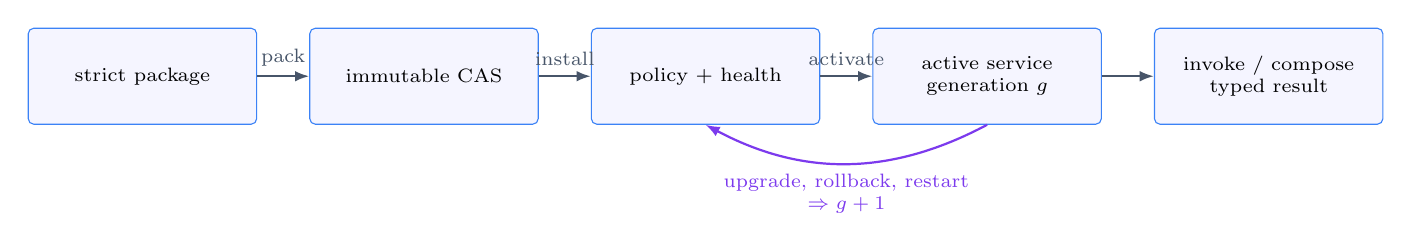
\begin{tikzpicture}[
  node distance=0.26in,
  n/.style={draw=OBlue,rounded corners=2pt,fill=blue!4,
    text width=1.05in,minimum height=0.48in,align=center,font=\scriptsize},
  a/.style={-{Latex[length=1.8mm]},thick,color=OSlate},
  r/.style={-{Latex[length=1.8mm]},thick,color=OPurple,bend left=28}
]
  \node[n] (pkg) {strict package};
  \node[n,right=of pkg] (cas) {immutable CAS};
  \node[n,right=of cas] (admit) {policy + health};
  \node[n,right=of admit] (active) {active service\\generation $g$};
  \node[n,right=of active] (invoke) {invoke / compose\\typed result};
  \draw[a] (pkg) -- node[above,font=\scriptsize]{pack} (cas);
  \draw[a] (cas) -- node[above,font=\scriptsize]{install} (admit);
  \draw[a] (admit) -- node[above,font=\scriptsize]{activate} (active);
  \draw[a] (active) -- (invoke);
  \draw[r] (active.south) to node[below,font=\scriptsize,align=center]
    {upgrade, rollback, restart\\$\Rightarrow g+1$} (admit.south);
\end{tikzpicture}
\caption{Admission and health create an executable Live-World generation.
Upgrade, rollback, and restart return through the gate and allocate a new
generation, making stale bearer identity explicit.}
\label{fig:live-state-machine}
\end{figure}

\subsection{KernelWorld authority chain}

\begin{figure}[htbp]
\centering
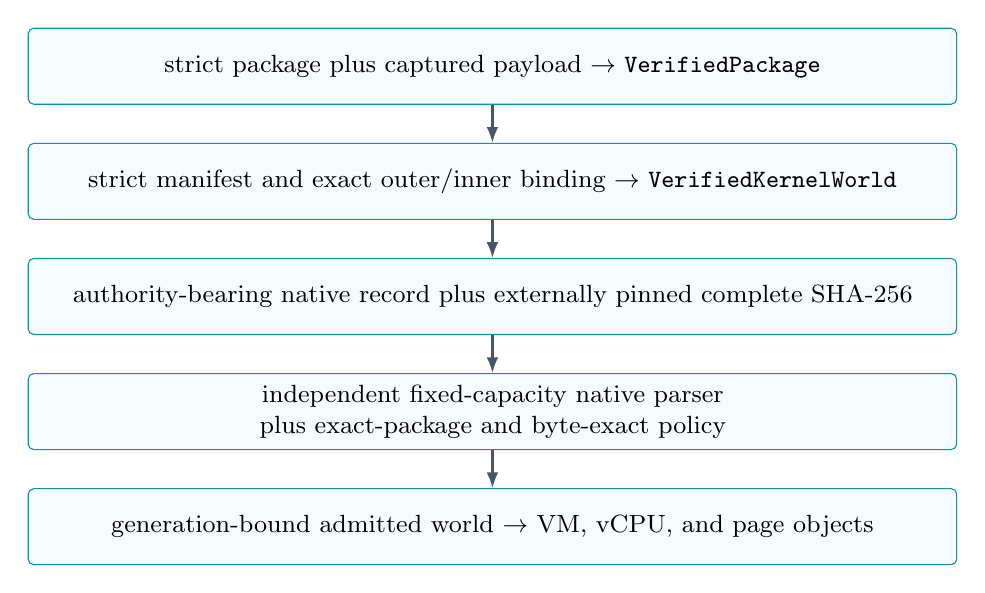
\begin{tikzpicture}[
  node distance=0.19in,
  n/.style={draw=OCyan,rounded corners=2pt,fill=cyan!4,
    minimum height=0.38in,text width=4.55in,align=center,font=\small},
  a/.style={-{Latex[length=2mm]},thick,color=OSlate}
]
  \node[n] (pkg) {strict package plus captured payload
    $\rightarrow$ \texttt{VerifiedPackage}};
  \node[n,below=of pkg] (world) {strict manifest and exact outer/inner binding
    $\rightarrow$ \texttt{VerifiedKernelWorld}};
  \node[n,below=of world] (record) {authority-bearing native record plus
    externally pinned complete SHA-256};
  \node[n,below=of record] (parse) {independent fixed-capacity native parser plus
    exact-package and byte-exact policy};
  \node[n,below=of parse] (grant) {generation-bound admitted world
    $\rightarrow$ VM, vCPU, and page objects};
  \draw[a] (pkg) -- (world);
  \draw[a] (world) -- (record);
  \draw[a] (record) -- (parse);
  \draw[a] (parse) -- (grant);
\end{tikzpicture}
\caption{KernelWorld verification and native admission.}
\end{figure}

Host verification joins the outer \texttt{ocore.package/v1} object to the
inner world manifest through exact equality. The outer runtime declares
\texttt{kind = "kernel-world"}; its ABI is
\path{ocore.kernel-world-control/v1}. Its absolute payload entry
names a non-executable UTF-8 manifest file. Outer and inner name, version,
architecture, health protocol, health timeout, service name/protocol set, and
normalized capability-request set match exactly. For a
\texttt{package\_payload} image, the declared SHA-256 equals the digest of the
exact image bytes opened from the verified payload. These equalities produce
one \texttt{VerifiedKernelWorld} bound to the immutable package digest. That
verified object creates the authority-bearing native record, whose native
codec checks every encoded bound exactly and rejects overflow.
\src{crates/ostadix-api/src/kernel_world.rs}{1--7}
\src{crates/ostadix-api/src/kernel_world.rs}{248--275}
\src{crates/ostadix-api/src/kernel_world.rs}{611--749}

The authorable KernelWorld manifest is strict TOML under
\texttt{ocore.kernel-world/v1}. Its required top-level fields are
\texttt{schema}, \texttt{name}, \texttt{version}, \texttt{integration},
\texttt{image}, \texttt{machine}, \texttt{lifecycle}, \texttt{quotas},
\texttt{exports}, \texttt{capability\_requests}, and \texttt{license}.

\begin{longtable}{P{0.20\textwidth} P{0.72\textwidth}}
\toprule
\textbf{Field group} & \textbf{Public vocabulary and cross-field contract} \\
\midrule
\endhead
Integration and image &
\texttt{source\_integrated} uses a \texttt{package\_payload} image,
\texttt{paravirtual} execution, and \texttt{direct} firmware.
\texttt{binary\_contained} uses \texttt{hardware\_virtualized} execution and
requests \texttt{vm.machine} \texttt{run} authority. Image kinds are
\texttt{package\_payload} with \texttt{path}/\texttt{sha256}, or
\texttt{user\_supplied} with \texttt{expected\_sha256}. \\
Machine &
\texttt{guest\_architecture}, \texttt{profile}, execution
\texttt{paravirtual}|\texttt{hardware\_virtualized}, firmware
\texttt{direct}|\texttt{uefi}, bounded min/max vCPUs and memory, and
requirements. \\
Lifecycle and quotas &
\texttt{health\_protocol}, \texttt{health\_timeout\_ms}, restart
\texttt{never}|\texttt{on\_failure}|\texttt{always}; outstanding requests,
requests per generation, shared-memory bytes, and device ceilings.
\texttt{max\_requests\_per\_generation} is at least
\texttt{max\_outstanding\_requests}. \\
Exports and authority &
Both lists are nonempty. Each export has \texttt{name}, plane
\texttt{device}|\texttt{abi}|\texttt{semantic}, and \texttt{protocol}. Each
capability request has \texttt{kind}, one or more \texttt{rights}, and
\texttt{purpose}. A device-plane export requires a \texttt{device.*} request
and a nonzero device quota. \\
License &
Redistribution is \texttt{redistributable}|\texttt{user\_supplied\_only},
paired with \texttt{external\_acceptance\_required}. A user-supplied image
selects \texttt{user\_supplied\_only} and requires external acceptance. \\
\bottomrule
\end{longtable}
\src{crates/ostadix-api/src/kernel_world.rs}{18--182}
\src{crates/ostadix-api/src/kernel_world.rs}{277--444}
\src{crates/ostadix-api/src/kernel_world.rs}{408--568}

The same public host contract includes \texttt{KernelWorldInstance}, a bounded
semantic oracle for lifecycle and request settlement. Its state path is
\texttt{Installed} $\rightarrow$ \texttt{Starting} $\rightarrow$
\texttt{Healthy}, with explicit \texttt{Failed} and \texttt{Stopped}
transitions. The manifest's \texttt{never}, \texttt{on\_failure}, or
\texttt{always} restart policy decides which terminal state may begin a fresh
generation. Healthy export resolution returns immutable package, world,
integration-mode, generation, and export provenance.

\begin{figure}[H]
\centering
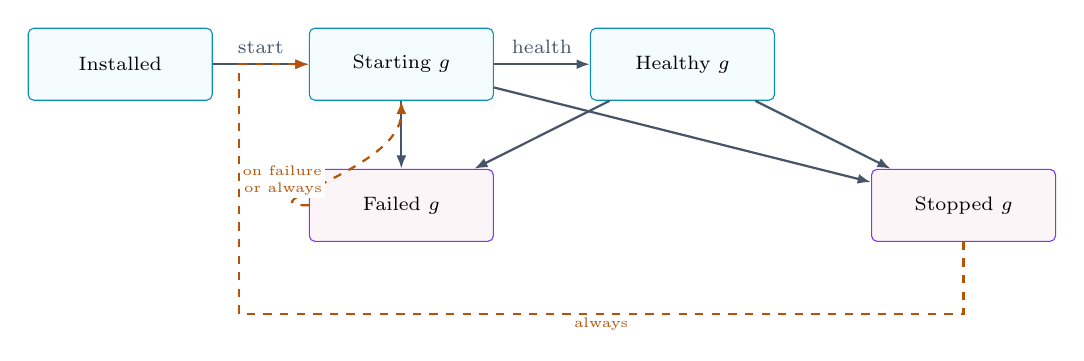
\begin{tikzpicture}[
  node distance=0.34in and 0.48in,
  s/.style={draw=OCyan,rounded corners=2pt,fill=cyan!4,
    minimum width=0.92in,minimum height=0.36in,align=center,font=\scriptsize},
  terminal/.style={s,draw=OPurple,fill=purple!4},
  a/.style={-{Latex[length=1.7mm]},thick,color=OSlate},
  r/.style={-{Latex[length=1.7mm]},thick,dashed,color=OAmber}
]
  \node[s] (installed) {Installed};
  \node[s,right=of installed] (starting) {Starting $g$};
  \node[s,right=of starting] (healthy) {Healthy $g$};
  \node[terminal,below left=of healthy] (failed) {Failed $g$};
  \node[terminal,below right=of healthy] (stopped) {Stopped $g$};
  \draw[a] (installed) -- node[above,font=\scriptsize]{start} (starting);
  \draw[a] (starting) -- node[above,font=\scriptsize]{health} (healthy);
  \draw[a] (starting) -- (failed);
  \draw[a] (starting) -- (stopped);
  \draw[a] (healthy) -- (failed);
  \draw[a] (healthy) -- (stopped);
  \draw[r] (failed.west) to[out=180,in=270,looseness=1.25]
    node[pos=0.48,left,font=\tiny,align=right,fill=white,inner sep=1pt]
      {on failure\\or always} (starting.south);
  \coordinate (restartStop) at ([yshift=-0.36in]stopped.south);
  \coordinate (restartLeft) at
    ([xshift=-0.35in,yshift=-0.36in]failed.south west);
  \draw[r] (stopped.south) -- (restartStop) --
    node[below,font=\tiny,fill=white,inner sep=1pt]{always}
    (restartLeft) |- (starting.west);
\end{tikzpicture}
\caption{The host-side KernelWorld lifecycle oracle. Restart policy controls
generation replacement, while health controls export publication.}
\label{fig:kernel-world-instance}
\end{figure}

Every \texttt{RequestId} is the pair $(generation, sequence)$. Outstanding and
per-generation quotas gate admission before insertion. Reply, cancellation,
deadline expiry, world failure, and world stop settle requests exactly once as
\texttt{Replied}, \texttt{Cancelled}, \texttt{DeadlineExceeded},
\texttt{WorldFailed}, or \texttt{WorldStopped}. Failure and stop drain all
in-flight requests into the corresponding terminal record; a replacement
generation resets the sequence and makes every earlier request ID stale.
\src{crates/ostadix-api/src/kernel_world.rs}{1208--1570}

Native admission consumes the deterministic normal form under an independently
registered immutable policy. It validates exact package identity and byte
content by kind and purpose, then creates a generation-bound grant after every
rule and cross-field constraint succeeds. The grant remains
\texttt{ADMITTED} until exact-generation revocation.
\src{ocore/runtime/x86_64/kernel_world_admission.oc}{1--11}
\src{ocore/runtime/x86_64/kernel_world_admission.oc}{1375--1478}
\src{ocore/runtime/x86_64/kernel_world_admission.oc}{1813--1934}

\subsection{Native execution ladder}

The native gates form one dependency-ordered execution ladder. Modes 0--20
establish the x86-64 bootstrap, isolation, process, scheduler, IPC, service,
personality, and KernelWorld prerequisites consumed by the later modes. Each
row names the new machine fact introduced at that point.

\begin{longtable}{P{0.10\textwidth} P{0.82\textwidth}}
\toprule
\textbf{Mode} & \textbf{Mode contract} \\
\midrule
\endhead
0 & Long-mode bootstrap, O-core kernel entry, serial output, allocator, IDT,
PIC/PIT, syscall entry, and one linked CPL3 personality. \\
1--8 & Fatal isolation probes for divide, invalid opcode, non-present access,
supervisor-page read, guard-stack access, NX instruction fetch, noncanonical
address, and invalid syscall return. \\
9 & Recoverable guarded \texttt{copy\_from\_user}/\texttt{copy\_to\_user} fault path. \\
10 & Normal process exit, exact lifecycle teardown, stale-handle denial, sibling
survival, and reclamation. \\
11 & Contained process-fault teardown with the unrelated sibling continuing. \\
12 & Four-TCB scheduler across two processes, preemption, yield, sleep/wake,
lifecycle, hostile saved-state containment, and one million identity switches. \\
13 & Kernel-side endpoint and capability-transfer foundation. \\
14 & Public CPL3 IPC with four-message FIFO blocking/wake, correlation,
attenuated transfer, death cleanup, and personality containment. \\
15 & Deterministic OVFS, static ELF loading, BSS/stack construction,
\texttt{W\textasciicircum X}
mappings, and service namespace. \\
16 & Four loaded service ELFs, serial activation, contained package-daemon
fault, health-gated restart, and final reclamation. \\
17 & Immutable package semantics, exact rollback, stale-generation denial,
restart, and control-parser behavior. \\
18 & Four-principal scalar personality RPC, unprivileged supervisor,
timeout/death settlement, restart, and exact capability rebind. \\
19 & Four request-scoped bounded-copy views, five lease classes, written-prefix
commit, terminal ordering, and delegated revocation. \\
20 & Exact KernelWorld record parsing, default-deny admission, and
generation-bound VM, vCPU, and guest-page object construction. \\
21 & AMD SVM/NPT synthetic-vCPU entry, controlled exit, injection, denied GPA,
teardown, and restart through the dedicated hardware gate. \\
\bottomrule
\end{longtable}

The implemented capacities make each native proof repeatable: 3,072 reclaiming
frames cover the fixed 4--16 MiB pool; M2 uses four TCBs, two processes, and
one CPU; M3 exposes four FIFO messages and 16 transfer tickets; M6A uses four
principals with 16 tombstones and nine retained identities; M6B provides four
views of 128 bytes each under a 256-byte aggregate charge and five lease
classes; Mode 20 constructs two VMs, four vCPUs, and eight guest pages.

The native artifact builders domain-separate OVFS, package, manifest, record,
and image identities. Each build gate recomputes those identities from the
exact current inputs and passes them to an independent validator before QEMU
consumes the artifact. Reproducers should retain the hashes printed by their
current-master run beside the gate transcript. Each source coordinate produces
its own artifact identities.

\src{ocore/kernel/build-m4-artifacts.sh}{1--40}
\src{ocore/kernel/build-m5-artifacts.sh}{1--40}
\src{ocore/kernel/build-m6-artifacts.sh}{1--40}

\subsection{Mode 20 and Mode 21}

\begin{longtable}{P{0.11\textwidth} P{0.38\textwidth} P{0.19\textwidth} P{0.20\textwidth}}
\toprule
\textbf{Gate} & \textbf{Implemented claim} & \textbf{Substrate} & \textbf{Execution significance} \\
\midrule
\endhead
Mode 20 &
Exact record validation, default-deny admission, generation-bound
nonexecuting VM/vCPU/pages, quota/overlap/stale/reclaim behavior. &
Portable x86 QEMU gate. &
Establishes the admission and object-construction stage before guest entry. \\
Mode 21 &
Real AMD SVM/NPT entry of a two-page synthetic real-mode guest, injected
vector, known computation, \texttt{VMMCALL}, denied unmapped GPA, teardown and
restart. &
Writable \texttt{/dev/kvm}, AMD SVM/NPT, QEMU KVM \texttt{-cpu host}. &
Defines the hardware execution gate for admitted objects and its required
execution substrate. \\
\bottomrule
\end{longtable}

\src{ocore/kernel/smoke-kernel-world-qemu.sh}{128--186}
\src{ocore/kernel/smoke-kernel-world-execution-qemu.sh}{8--177}
\src{ocore/runtime/x86_64/svm_execution.oc}{24--507}

\subsection{Modes 22 through 34}
\label{sec:modes22-34}

Modes 22 through 34 extend the portable evidence ladder through supervised
KernelWorld execution, bounded foreign-personality services, canonical World
records, causal fallback, hosted-to-native receipt convergence, challenged
boot information, and four-CPU startup. All thirteen modes are required gates
in the current evidence registry.

\begin{longtable}{P{0.08\textwidth} P{0.51\textwidth} P{0.33\textwidth}}
\toprule
\textbf{Mode} & \textbf{Implemented mechanism} & \textbf{Required gate} \\
\midrule
\endhead
22 & Health-gated typed export publication, reset intent, failure withdrawal,
exact VM-graph revocation, generation-2 restart, stale-generation denial, and
unrelated-service survival. &
\breakcode{smoke-kernel-world-live-qemu.sh} \\
23 & TCG-emulated SVM/NPT entry, VMEXIT-derived health, validated virtual PIO,
NPF quiescence, execution-pin release, generation rebind, and cross-World
authority rejection. &
\breakcode{smoke-kernel-world-execution-device-qemu.sh} \\
24 & Four digest-pinned CPL3 bounded-personality services, terminal lifecycle
matrix, contained daemon fault, generation replacement, and request-wide
authority cleanup. &
\breakcode{smoke-live-bounded-personality-qemu.sh} \\
25 & Exact static Linux x86-64 ELF execution in CPL3 through a four-call
personality, stdout/stderr results, exact \texttt{-ENOSYS}, exit status,
replacement, and resource reclamation. &
\breakcode{smoke-live-linux-personality-qemu.sh} \\
26 & Native Linux 9P2000 provider and Plan-9-style client over the exact
\path{/srv/linux/status} exchange, namespace withdrawal, provider replacement,
stale denial, and reclamation. &
\breakcode{smoke-live-linux-plan9-qemu.sh} \\
27 & Shared Rust and O-core World identity types, byte-identical OWIDENT V1
corpus, nonzero coordinate validation, and hierarchical stale and logical
comparison. &
\breakcode{smoke-world-identity-qemu.sh} \\
28 & OWPROTO V1 big-endian records, exact bounds and fields, deterministic
version negotiation, and Rust/O-core byte convergence. &
\breakcode{smoke-world-protocol-qemu.sh} \\
29 & OWVALUE V1 portable allowlist, bounded recursive shape, canonical ordering,
authority-bearing value rejection, stable hashing, and cross-language byte
convergence. &
\breakcode{smoke-world-value-qemu.sh} \\
30 & OWRECEIPT V1 canonical receipt and signing preimage, hosted Ed25519
sign/verify, structural signature-envelope validation, World generation and
commit fields, and Rust/O-core byte convergence. &
\breakcode{smoke-world-receipt-qemu.sh} \\
31 & One LogicalRead across generation-distinct providers, terminal A failure,
A-route withdrawal, fresh B-local session reconstruction, immutable object
hash validation, causal attempt state, cleanup, and witness survival. &
\breakcode{smoke-m7b-logical-read-qemu.sh} \\
32 & Hosted project execution through a caller-supplied World view, live signed
uncommitted receipt emission, native full decode and exact re-encode, signing
preimage reconstruction, and signer-independent semantic digest equality. &
\breakcode{smoke-world-project-runtime-qemu.sh} \\
33 & Challenged UEFI/Multiboot2 handoff into bounded kernel-owned BootInfo,
memory-map-selected allocator window, retired inspection aperture, CPL3
lifecycle, and transcript challenge binding. &
\breakcode{smoke-x86\_64-boot-info-qemu.sh} \\
34 & Exact four-CPU ACPI/MADT topology, PIT progress, x2APIC INIT/SIPI, distinct
AP stacks, trampoline \texttt{W\textasciicircum X} lifecycle, one atomic
BSP/AP barrier, post-barrier
timer, and one-CPU rejection control. &
\breakcode{smoke-x86\_64-smp-qemu.sh} \\
\bottomrule
\end{longtable}

\begin{figure}[htbp]
\centering
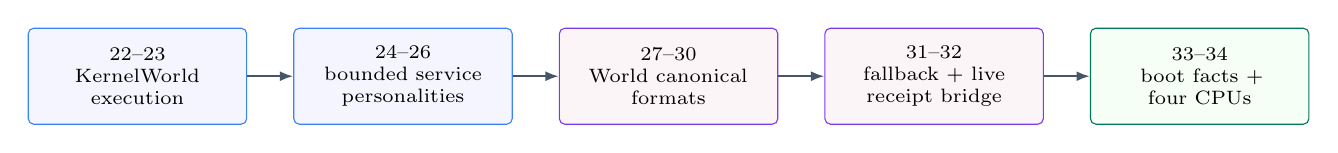
\begin{tikzpicture}[
  node distance=0.23in,
  m/.style={draw=OBlue,rounded corners=2pt,fill=blue!4,
    text width=1.00in,minimum height=0.48in,align=center,font=\scriptsize},
  w/.style={draw=OPurple,rounded corners=2pt,fill=purple!4,
    text width=1.00in,minimum height=0.48in,align=center,font=\scriptsize},
  p/.style={draw=OGreen,rounded corners=2pt,fill=green!4,
    text width=1.00in,minimum height=0.48in,align=center,font=\scriptsize},
  a/.style={-{Latex[length=1.7mm]},thick,color=OSlate}
]
  \node[m] (m22) {22--23\\KernelWorld\\execution};
  \node[m,right=of m22] (m24) {24--26\\bounded service\\personalities};
  \node[w,right=of m24] (m27) {27--30\\World canonical\\formats};
  \node[w,right=of m27] (m31) {31--32\\fallback + live\\receipt bridge};
  \node[p,right=of m31] (m33) {33--34\\boot facts +\\four CPUs};
  \foreach \x/\y in {m22/m24,m24/m27,m27/m31,m31/m33}
    {\draw[a] (\x) -- (\y);}
\end{tikzpicture}
\caption{Modes 22 through 34 move from supervised execution through portable
World records and causal recovery into challenged platform initialization.}
\label{fig:modes22-34}
\end{figure}

The evidence registry declares its schema, required count, supplemental count,
portable aggregate command, per-gate tool requirements, positive claims, and
expected transcript markers. The validator checks registry structure,
required membership, script presence, evidence classes, milestone uniqueness,
marker discipline, and the release projection consumed by the portable
aggregate. Mode 32 additionally wires a focused hosted project execution test
into the native receipt gate so the receipt being checked originates from an
executed Project HGraph path.

\src{evidence/gates.toml}{1--4}
\src{evidence/gates.toml}{674--684}
\src{evidence/gates.toml}{697--707}
\src{evidence/gates.toml}{468--478}
\src{evidence/gates.toml}{497--507}
\src{evidence/gates.toml}{531--541}
\src{evidence/gates.toml}{103--113}
\src{evidence/gates.toml}{125--135}
\src{evidence/gates.toml}{148--158}
\src{evidence/gates.toml}{174--184}
\src{evidence/gates.toml}{579--589}
\src{evidence/gates.toml}{205--215}
\src{evidence/gates.toml}{29--40}
\src{evidence/gates.toml}{52--63}
\src{scripts/release_evidence.py}{20--29}
\src{scripts/release_evidence.py}{118--291}
\src{scripts/release_evidence.py}{487--586}
\src{ocore/kernel/smoke-world-project-runtime-qemu.sh}{16--35}
\src{tests/project_world_runtime.rs}{359--449}

\section{Reproducibility and current-master evidence}
\label{sec:validation}

This paper pins source identity before interpreting output. The current
qualification coordinate is commit
\texttt{36787b16476bc0c8c4ddf665c7228b314d04e716}, package
\texttt{0.4.0 Unreleased}. Every result below belongs to that coordinate or to
an artifact derived from it.

\subsection{Evidence classes}

A reader should distinguish four kinds of evidence used in this paper:

\begin{enumerate}
  \item \textbf{Defining source.} Narrow file and line citations identify the
        implementation that makes a claim true.
  \item \textbf{Generated structure.} Compiler output exposes the exact
        program graph in the compiler's own vocabulary.
  \item \textbf{Registry validation.} The evidence validator checks the
        declared gate inventory and the portable release projection.
  \item \textbf{Execution transcripts.} Each registered gate defines required
        tools and expected markers for its actual execution substrate.
\end{enumerate}

This order matters. Source establishes the mechanism. Generated structure
shows the mechanism instantiated for a program. Registry validation establishes
the release's required proof surface. Execution transcripts establish that a
particular substrate completed the registered gate.

\subsection{Current snapshot checks}

\begin{longtable}{P{0.27\textwidth} P{0.25\textwidth} P{0.40\textwidth}}
\toprule
\textbf{Check} & \textbf{Observed current result} & \textbf{Meaning} \\
\midrule
\endhead
\texttt{git rev-parse HEAD} &
\breakcode{36787b16476bc0c8c4ddf665c7228b314d04e716} &
Pins every source citation and generated artifact in this paper. \\
Root package coordinate &
\texttt{o-lang 0.4.0}; changelog state \texttt{Unreleased}. &
Names the synchronized development package and its release state. \\
Workspace ownership &
Two default members; exact \texttt{ostadix-api =0.4.0} dependency; separately
locked MCP root excluded. &
Confirms the engine, CLI shell, and MCP dependency boundaries. \\
Public binary boundary &
All fourteen binaries executed: thirteen printed their public help; the
notebook served its loopback UI, evaluated \texttt{text\string^(42\string)\_text}
as typed text \texttt{"42"}, and completed reset. &
Exercises every declared root binary through a safe public entry boundary. \\
Root Rust quality gates &
\status{OGreen}{Formatting, check, and Clippy passed}. &
Qualifies the synchronized root and engine workspace under the current feature
surface. \\
Release binary surface &
\status{OGreen}{All workspace binaries built with all features and the locked
dependency graph in 3 minutes 13 seconds}. &
Qualifies the optimized deployable command surface independently from test
harness compilation. \\
Rust test inventory &
\status{OGreen}{1,351 passed, 3 ignored} across 62 harnesses; 1,354 tests
listed. &
Exercises all targets and features across hosted semantics, evidence,
projects, networking, Information, Registry, World, Live-World, KernelWorld,
and \ocore{} host contracts. \\
MCP Rust package &
\status{OGreen}{Build and Clippy passed; 29 Rust tests passed; ten-tool smoke
passed}. &
Qualifies the separately locked MCP package and every declared tool route. \\
Python reference &
\status{OGreen}{18 of 18 parser tests and 46 of 46 evaluator tests passed};
\texttt{compileall} passed. &
Exercises the reference grammar, evaluator, and importable source tree. \\
C17 edition &
\status{OGreen}{Make manifest: 5 passed; AOT manifest: 3 passed, 2 manifest
skips; safety gate passed; CMake/CTest: 4 of 4 passed}. &
Qualifies the standalone interpreter, generated-C path, and both build-system
surfaces. \\
Examples &
\status{OGreen}{39 Rust example runs passed, 5 manifest skips; recursive
manifest accounted for 44 examples}. &
Exercises the tracked hosted teaching corpus under its declared platform
requirements. \\
Source release &
\status{OGreen}{77 of 77 source-release checks passed}. &
Qualifies the current tracked source projection, package boundaries, and
archive rules. \\
\texttt{olangc} target matrix &
\status{OGreen}{All five targets completed their compilation or emission
contract; binary and script targets also executed}. &
Exercises host binary generation and execution, WASI generation, direct
script execution, IR inspection, and DOT graph emission. \\
Project, Live, and World smokes &
\status{OGreen}{Project HGraph, project execution, Hosted Live-World, and
World smoke families passed}. &
Connects logical planning to execution, lifecycle supervision, World codecs,
and receipt paths. \\
Docker probe &
\status{OGreen}{Passed}. &
Qualifies the maintained container build and hosted probe boundary. \\
MCP tool inventory &
Ten \texttt{\#[tool]} definitions. &
Confirms the complete agent-facing operation vocabulary listed in
Section~\ref{sec:mcp}. \\
Project lift &
7,501 bytes; SHA-256
\breakcode{a6d97fd5b95b829c3e3a754722767960f2963e0644ba8c89da7c15d48d922bb1}. &
Pins the o-linked project artifact used by the graph illustration. \\
Project DOT &
13,065 bytes; SHA-256
\breakcode{bf16748f53a377e950a67b9c27d48ff260dcc987a69d86c5f29ca6289df7f00b};
direct directory and lifted input byte-identical. &
Confirms reversible project lifting at the compiler's logical graph boundary. \\
Rendered graph &
53 semantic vertices, 62 directed edges; vector PDF SHA-256
\breakcode{75c7d219d208a2afddc51a5c9c682c506d26cd9729145828019f88f1c6a8e90e}. &
Pins the complete landscape figure and its reading guide. \\
\texttt{python3}\newline
\texttt{scripts/}\newline
\texttt{release\_evidence.py}\newline
\texttt{validate} &
\status{OGreen}{\texttt{release evidence: PASS (26 required portable QEMU gates)}}. &
Validates the current evidence registry and its 26-gate portable projection. \\
Portable QEMU aggregate &
\status{OGreen}{26 of 26 required gates passed; 201 expected markers matched;
361.11 seconds}. &
Executes the complete current portable native evidence ladder, including every
required Mode 22 through Mode 34 gate. \\
\bottomrule
\end{longtable}

\src{Cargo.toml}{1--18}
\src{Cargo.toml}{78--86}
\src{CHANGELOG.md}{8--50}
\src{mcp/ostadix_lang_mcp_server/src/main.rs}{1663--2207}
\src{evidence/gates.toml}{1--4}
\src{scripts/release_evidence.py}{487--586}

\subsection{Exact reproduction commands}

\begin{lstlisting}[style=plaincode]
git rev-parse HEAD
# 36787b16476bc0c8c4ddf665c7228b314d04e716

cargo build --release --workspace --bins --all-features --locked

python3 scripts/release_evidence.py validate
# release evidence: PASS (26 required portable QEMU gates)

rg -n '^\s*#\[tool\(' mcp/ostadix_lang_mcp_server/src/main.rs
# ten tool definitions

mkdir -p output/current-master
./target/release/o-link tests/fixtures/project_hgraph --project \
  -o output/current-master/o-linked-project.O
./target/release/olangc output/current-master/o-linked-project.O \
  --target dot --route main --shim-dir backends \
  > output/current-master/o-linked-codebase-hgraph.dot
./target/release/olangc tests/fixtures/project_hgraph \
  --target dot --route main --shim-dir backends \
  > output/current-master/project-hgraph-direct.dot
cmp output/current-master/o-linked-codebase-hgraph.dot \
    output/current-master/project-hgraph-direct.dot
cp output/current-master/o-linked-codebase-hgraph.dot \
  docs/figures/o-linked-codebase-hgraph.dot
dot -Tsvg output/current-master/o-linked-codebase-hgraph.dot \
  -o docs/figures/o-linked-codebase-hgraph.svg
dot -Tpdf output/current-master/o-linked-codebase-hgraph.dot \
  -o docs/figures/o-linked-codebase-hgraph.pdf
shasum -a 256 \
  output/current-master/o-linked-project.O \
  output/current-master/o-linked-codebase-hgraph.dot \
  docs/figures/o-linked-codebase-hgraph.dot \
  docs/figures/o-linked-codebase-hgraph.svg \
  docs/figures/o-linked-codebase-hgraph.pdf
\end{lstlisting}

The current gate registry names the portable aggregate as:

\begin{lstlisting}[style=plaincode]
./boot-and-test.sh smoke
\end{lstlisting}

That aggregate consumes the registry projection checked above. Individual mode
scripts remain directly runnable and name their expected markers in
\path{evidence/gates.toml}. This gives a reproducer one route from the release
coordinate, through registry qualification, into each concrete hosted or QEMU
execution transcript.

\subsection{Coverage accounting}

The current public surface is accounted for through explicit inventories:
fourteen root binaries; one independent engine package; ten MCP tools; four
current execution coordinates in Graph V2, Evidence V6, Admission V6, and Why
V2; eight Information Bridge projections; three Registry V1 event bodies; four
World wire families; thirteen required modes from 22 through 34; and the
twenty-six-gate portable evidence registry. The sections and appendices map
each inventory to defining source and the command that exposes it.

\section{Implemented capabilities}
\label{sec:claims}

\begin{itemize}
  \item A structural polyglot syntax with exact language-tagged nesting,
        persistent environments, bindings, calls, quotation, and scopes.
  \item A rich typed interchange algebra with explicit fidelity metadata and a
        canonical CBOR wire protocol capped at 128 MiB per frame.
  \item Uniform hosted lowering through \oir{}, a validated plan, and a
        state-complete \hgraph{}.
  \item Deterministic graph settlement with explicit resource/effect
        modeling and verified-inline parallelism.
  \item Deferred requests, Nix/OS values, and four first-class group
        topologies.
  \item Explicit route-preserving project lifting, reversible project bundles,
        logical Project HGraphs, executable route policies, and capacity-first
        Project Mesh placement.
  \item Hosted packaging to native host executables and WASI modules, plus
        separate Python and C17 reference/subset editions.
  \item A distinct freestanding \ocore{} compiler and native x86-64/AArch64
        kernel substrates, including challenged x86-64 BootInfo and bounded
        four-CPU startup.
  \item Hosted Live-World supervision and a strict KernelWorld record/admission
        contract.
  \item An independently packageable \texttt{ostadix-api} engine, an exact
        root compatibility shell, a unified lowercase \texttt{o} command, and
        a ten-tool local MCP.
  \item Graph V2 identity, Evidence V6 analysis, Admission V6 authority, Why V2
        explanation, and one-use agent intent handles.
  \item Reciprocal SPAKE2 pairing, destination-issued credentials, pinned TLS,
        Registry V1 profiles, and generation-fenced mesh execution.
  \item Content-addressed Information, eight bounded native projections,
        typed provenance recovery, and canonical World identity, protocol,
        value, and receipt formats.
\end{itemize}

\section{Design rationale}
\label{sec:assessment}

\subsection{Why evaluator identity is syntax}

I made evaluator identity part of syntax because the composition point is a
semantic boundary. Structural recognition preserves native backend source
while giving the host a complete heterogeneous program tree. The notation
therefore carries both the foreign program and the information required to
compose it.

\subsection{Why graph state is explicit}

Execution semantics include values, failures, ordering, actor mutation, and
world effects. I represent those dimensions with ordinary values, completion
tokens, and versioned resource nodes. This ontology preserves observable
serial behavior while admitting a precise parallel frontier, making
state-complete graph projection the architectural center of the hosted
runtime.

\subsection{Why analysis and authority are separate objects}

I separate Graph V2 identity, Evidence V6 analysis, and Admission V6 authority
because each stage answers a different technical question. Graph V2 states
which solved computation exists. Evidence V6 states why each operation is
executable in one exact context. Admission V6 proves that the context and
analysis still reproduce at the execution boundary. Why V2 exposes the
resulting dependency neighborhood in a stable reader-facing form. This
separation gives compilers, local commands, agents, and placement systems one
shared execution constitution.

\subsection{Why the engine owns the types}

I made \texttt{ostadix-api} the implementation owner so embedding is a primary
runtime surface. Parser nodes, \ovalue{}, plans, graphs, evidence, admission,
projects, and World records can be used directly without importing a command
package. The root crate reexports those exact identities, preserving existing
programs while keeping one evaluator and one value universe.

\subsection{Why admission is typed across layers}

I use one typed admission architecture across hosted and native execution.
Hosted Live-World executes the lifecycle semantics and supplies a differential
oracle for native World stages. Native M5 realizes an isolated service
lifecycle on its own substrate. The connected authority path begins when
KernelWorld binds verified package bytes, manifest claims, and policy into a
deterministic record. The native parser verifies that record, Mode 20
constructs generation-bound admission objects from it, and Mode 21 consumes an
admitted object at guest entry. This path carries authority through explicit
verification products while the hosted and native lifecycle implementations
share the same semantic vocabulary.

\subsection{Why placement begins with capacity}

Project Mesh begins with usable execution capacity because placement exists to
increase the amount of work the language can execute. It ranks paired node
profiles by capacity, then applies compatibility, generation, route, and
policy constraints to the source-closed branch. Admission records, reciprocal
TLS identity, and causal attempt traces make that capacity dependable at the
moment it is used.

\section{Conclusion}

I designed \product{} around one proposition: evaluator identity belongs in
the structural syntax of a typed expression. That decision gives the parser a
heterogeneous program tree, gives \ovalue{}
a typed boundary between independent runtimes, and gives \oir{}/\hgraph{} the
information required to represent dataflow, completion, actor state, and
world effects explicitly. The nesting is the interface because the nesting
survives every stage from source recognition to runtime settlement.

The project layer extends the same idea from expressions to complete source
trees. Deterministic bundles preserve artifacts, route policies select whole
execution alternatives, and the toolchain exposes their complete logical
Project HGraph. Project Mesh closes a selected branch over its prerequisites,
ranks paired nodes by capacity, and binds every attempt to node generations
and returned artifacts.

\ocore{} carries the architecture to the machine boundary. Typed source lowers
through HIR and SSA MIR into freestanding x86-64 objects, which compose into a
kernel with generation-tagged capabilities, isolated native services, strict
KernelWorld records, and staged VM admission and entry. Hosted Live-World
supplies executable lifecycle semantics for immutable packages, service
generations, revocation, rollback, and reconstruction.

The result is one language system spanning recursive polyglot programming,
state-complete graph execution, whole-project composition, native compilation,
capability-bearing kernel services, Information, Registry, and World
construction. The independent engine, unified \texttt{o}, and ten-tool MCP
make the same runtime available to embedders, operators, and agents. Graph V2,
Evidence V6, Admission V6, and Why V2 carry one continuous representation of
evaluator choice, typed value, effect, explanation, authority, and execution
substrate across all of those scales.

\appendix

\section{Compact hosted-language reference}

\begin{longtable}{P{0.35\textwidth} P{0.57\textwidth}}
\toprule
\textbf{Form} & \textbf{Meaning} \\
\midrule
\endhead
\texttt{LANG\string^(body\string)\_LANG} &
Fresh ephemeral evaluator expression. \\
\texttt{LANG[n]\string^(body\string)\_LANG[n]} &
Persistent evaluator actor keyed by language, numeric ID, and process policy. \\
\texttt{LANG\{lazy\}\string^(...\string)\_LANG\{lazy\}} &
Cache-safe deferred inline evaluation; auto-forces on splice. \\
\texttt{LANG\{defer\}\string^(...\string)\_LANG\{defer\}} &
Non-cacheable deferred evaluation; requires explicit \texttt{now}. \\
\texttt{let x = expr} &
Root binding store; right-hand side is a typed block or orchestration call. \\
\texttt{\$x} &
Load and splice the visible binding. \\
\texttt{quote\string^(...\string)\_quote} &
Produce an unevaluated \texttt{OExpr}. \\
\texttt{O.eval(expr[, scope])} &
Shim callback that reparses and evaluates quoted O source. \\
\texttt{scope()}, \texttt{O.scope()} &
Capture the visible O lexical environment as an \texttt{OScope}. \\
\texttt{lazy(x)}, \texttt{autonomous(x)}, \texttt{now(x)} &
Demand-policy and forcing operations. \\
\texttt{batch/all/any/race(...)} &
First-class group construction with distinct settlement rules. \\
\texttt{instantiate}, \texttt{realise}, \texttt{activate} &
Move through Nix expression, derivation, store path, and system rungs. \\
\texttt{dry\_activate}, \texttt{current\_system} &
Construct an activation result without mutation; inspect the current system
value. \\
\texttt{cap=}, authority flags, \texttt{effects=}, \texttt{reads=},
\texttt{writes=}, \texttt{serial=host} &
Attach capability, effect, resource, and serialization metadata to a block. \\
\bottomrule
\end{longtable}

\subsection{Exact builtin signatures}

\begin{longtable}{P{0.38\textwidth} P{0.54\textwidth}}
\toprule
\textbf{Signature} & \textbf{Value transition} \\
\midrule
\endhead
\texttt{instantiate(expr)} & \texttt{ONixExpr} to
\texttt{ODerivation}. \\
\texttt{realise(drv)} & \texttt{ODerivation} to
\texttt{OStorePath}. \\
\texttt{now(request\_or\_group)} & Force one request chain or settle one
coordination group. \\
\texttt{dry\_activate(path[, profile])} & Construct the dry activation result
for one store path and optional profile. \\
\texttt{activate(path[, profile])} & Activate with ambient system authority. \\
\texttt{activate(}\newline
\texttt{system\_activation\_capability,}\newline
\texttt{path[, profile])} & Validate the typed activation capability and
profile guard, then activate. \\
\texttt{current\_system()} & Return the current referential
\texttt{OSystem}. \\
\texttt{scope()} & Capture visible O bindings as a detached
\texttt{OScope}. \\
\texttt{lazy(expr)} & Evaluate one expression under Lazy policy. \\
\texttt{autonomous(expr)} & Evaluate one expression under Autonomous policy
and flush admitted work. \\
\texttt{batch(a,...)}, \texttt{all(a,...)}, \texttt{any(a,...)},
\texttt{race(a,...)} & Capture an ordered member list with the selected
settlement topology. \\
\bottomrule
\end{longtable}

\Needspace{10\baselineskip}
\section{Public command reference}

\begin{longtable}{P{0.18\textwidth} P{0.42\textwidth} P{0.32\textwidth}}
\toprule
\textbf{Command} & \textbf{Principal forms} & \textbf{Result} \\
\midrule
\endhead
\texttt{O} & \texttt{O [--executor serial|graph] [--workers N]
[--backend-grant SPEC] [--json] [--check] FILE [shim-dir]};
\texttt{O --eval SOURCE} or \texttt{O -e SOURCE};
\texttt{--require-source-sha256 HEX};
\texttt{--require-execution-intent-sha256 HEX};
\texttt{O --repl [shim-dir]}; no arguments in an interactive terminal;
\texttt{-i} aliases \texttt{--repl}; \texttt{O --version};
\texttt{O version [--json]}; \texttt{-h}/\texttt{--help}; REPL commands
\texttt{:scope}, \texttt{:r}, \texttt{:?}, \texttt{:q} &
Evaluate one document or enter and control the persistent interactive session. \\
\texttt{o} dispatcher &
\texttt{run}, \texttt{plan}, \texttt{explain}, \texttt{inspect},
\texttt{why}, \texttt{kernel}, \texttt{node}, \texttt{node-host},
\texttt{registry}, \texttt{info}, \texttt{live}, and \texttt{receipt};
all other forms enter \texttt{O} &
Route one lowercase command surface into the compiled intent front door,
compiler inspection, kernel, node, Registry, Information, Live-World, O-Git,
or ordinary evaluator. \\
\texttt{o-cli} &
\texttt{o run INPUT [execution options]};
\texttt{o plan INPUT [--route ID] [--live]};
\texttt{o explain [last-run|RUN] [--json]};
\texttt{o inspect [last-run|RUN] [--trace] [--json]} &
Resolve one hosted or project intent, plan or execute it, and retain a durable
run record for explanation and inspection. \\
\texttt{olangc} & \texttt{--target binary|wasm|script|ir|dot};
\texttt{-o}/\texttt{--output}; \texttt{--shim-dir};
\texttt{--keep-build-dir}; repeatable
\texttt{--backend-grant}; \texttt{--route}; \texttt{--routes-policy};
\texttt{--project-trace-out}; \texttt{--grounding};
\texttt{--explain-schedule}; \texttt{--format};
\texttt{--execution-intent-json}; \texttt{--why}; \texttt{--workers};
\texttt{--world-id}; \texttt{--world-epoch} &
Package, execute, or inspect the hosted graph. Script target executes
immediately inside the compiler process. \\
\texttt{ocorec} & One or more input modules; \texttt{--emit
ast|hir|mir|asm|obj}; \texttt{--target x86\_64-unknown-none[-elf]} or
\texttt{aarch64-unknown-none[-elf]}; \texttt{-o}/\texttt{--output};
\texttt{--keep-asm}; \texttt{-V}/\texttt{--version} &
Inspect or compile the complete O-core pipeline. \\
\texttt{o-link} & Bare single-directory literal run; explicit
\texttt{--literal} link; explicit \texttt{--project} project lift;
\texttt{-o}/\texttt{--output};
\texttt{--stdout}; repeatable \texttt{--lang}; \texttt{--verbose-skips};
\texttt{--no-validate}; \texttt{--run}; \texttt{--shim-dir};
\texttt{--backend-grant}; \texttt{--shebang};
\texttt{--list-routes}; \texttt{--route}; \texttt{--routes-policy};
repeatable \texttt{--route-decl}; \texttt{--project-trace-out};
\texttt{--parallel[=verified]}; \texttt{--parallel-required};
\texttt{--explain-parallel}; \texttt{--mesh[=prefer|required]};
\texttt{--mesh-retries}; \texttt{--mesh-local-fallback};
\texttt{--mesh-discovery-timeout-ms}; \texttt{--mesh-no-lan-discovery};
\texttt{--mesh-peer-root}; \texttt{--mesh-trace-out};
\texttt{--explain-mesh} &
Create reversible project or literal artifacts and invoke selected routes. \\
Generated project binary & No argument for its selected default;
\texttt{--list-routes}; \texttt{--route ID}; \texttt{--routes-policy POLICY} &
Restore the embedded project and execute its route coordinator. \\
\texttt{o-unlink} & \texttt{o-unlink input.O
(-o|--output-dir) dir}; \texttt{--dry-run} &
Restore either embedded representation with format-specific validation. \\
\texttt{o-notebook} & \texttt{o-notebook [shim-dir]} &
Serve the embedded loopback notebook and its shared evaluator session. \\
\texttt{ogit} & \texttt{demo semantic-receipt}; \texttt{diff-semantic A B} &
Generate a semantic receipt or compare group policy and intent. \\
\texttt{o-live-host} & \texttt{pack}, \texttt{install}, \texttt{activate},
\texttt{invoke}, \texttt{compose}, \texttt{upgrade}, \texttt{rollback},
\texttt{restart}, \texttt{status}, \texttt{demo} &
Drive the complete hosted lifecycle state machine. \\
\texttt{o-node} & \texttt{start}, \texttt{stop}, \texttt{status},
\texttt{restart}, \texttt{pair}, \texttt{pki}, \texttt{identity},
\texttt{admin}, \texttt{profile}, \texttt{doctor}, \texttt{serve} &
Run the node service, establish reciprocal identity pins, and administer its
bounded hosted execution state. \\
\texttt{octl} & \texttt{node list}, \texttt{node use},
\texttt{node profile}, \texttt{node doctor}, \texttt{node run},
\texttt{node session}, \texttt{node authority} &
Discover and select paired nodes, invoke exact source, operate durable
sessions, and issue development-authority leases. \\
\texttt{o-registry} & \texttt{init}, \texttt{profile-local},
\texttt{publish-profile}, \texttt{verify}, \texttt{list}, \texttt{export},
\texttt{import} &
Operate the local signed Registry V1 event chain. \\
\texttt{o-info} & \texttt{init}, \texttt{keygen}, \texttt{record},
\texttt{verify}, \texttt{import}, \texttt{head} &
Create, sign, verify, import, and inspect bounded content-addressed
Information state. \\
\texttt{ocore-kernel-}\newline\texttt{world-record} &
\texttt{--manifest}; \texttt{--payload}; \texttt{-o}/\texttt{--output};
\texttt{-V}/\texttt{--version} &
Verify one package/payload pair, encode its deterministic native admission
record, and print its bytes, path, record hash, and package digest. \\
Python 0.4.0 & \texttt{python3 -m o\_lang FILE}; \texttt{--as
auto|text|html|markdown|latex|json}; \texttt{-o}/\texttt{--output};
\texttt{--dump-ast}; \texttt{-V}/\texttt{--version}; typed root API above &
Execute the source-tree reference edition or consume typed Python API values. \\
C17 edition & \texttt{c\_cpp/O INPUT.O [shim-dir]};
\texttt{c\_cpp/olangc INPUT.O [-o OUT] [--shim-dir DIR]
[--keep-build-dir]} &
Run or AOT-compile the standalone C17 hosted edition. \\
Setup and aggregate gates & \texttt{setup.sh} with
\texttt{-m}/\texttt{--minimal}, \texttt{-f}/\texttt{--full},
\texttt{-y}/\texttt{--yes}, \texttt{-v}/\texttt{--verify},
\texttt{--no-wrappers}, \texttt{--dry-run}, \texttt{-h}/\texttt{--help};
\texttt{boot-and-test.sh}
phases \texttt{setup}, \texttt{hosted}, \texttt{ocore}, \texttt{kernel},
\texttt{smoke}, \texttt{tests}, \texttt{quick}, \texttt{full} &
Build, install, verify, or execute the repository-wide layer gates. \\
\texttt{fuzz/parser} & \texttt{cargo fuzz run parser} &
Feed arbitrary bytes through the hosted parser under libFuzzer. \\
\bottomrule
\end{longtable}

\src{src/main.rs}{15--80}
\src{src/main.rs}{303--337}
\src{scripts/o-cli.sh}{18--116}
\src{src/bin/olangc.rs}{192--257}
\src{crates/ostadix-api/src/ocore/driver.rs}{11--35}
\src{src/bin/olink.rs}{155--374}
\src{o_lang/cli.py}{123--141}

Thirteen root binaries expose \texttt{-h}/\texttt{--help} at their public
command boundary. The notebook serves its positional loopback interface at
\texttt{127.0.0.1:8888}. The historical C17 help behavior is recorded in the
final boundary table.

Every stateful \texttt{o-live-host} command accepts global optional
\texttt{--policy FILE}. Its exact subcommand arguments are:

\begin{lstlisting}[style=plaincode]
pack --manifest MANIFEST --payload PAYLOAD
install --state STATE --manifest MANIFEST --payload PAYLOAD [--alias ALIAS]
activate --state STATE DIGEST
upgrade --state STATE DIGEST
invoke --state STATE SERVICE PROTOCOL OPERATION INPUT
compose --state STATE --plan PLAN --input INPUT
rollback --state STATE PACKAGE
restart --state STATE SERVICE
status --state STATE
demo --state STATE
\end{lstlisting}

\section{Example atlas}

The example atlas has ten families. The 42 tracked top-level
\texttt{examples/*.O} files form nine executable teaching families. Companion
fixtures in \path{examples/group_pipeline/},
\path{tests/fixtures/project_hgraph/}, and
\path{tests/fixtures/project_hgraph_exec/} form the tenth through semantic
receipts, logical project graphing, and bounded project execution.

\begin{longtable}{P{0.24\textwidth} P{0.28\textwidth} P{0.40\textwidth}}
\toprule
\textbf{Family} & \textbf{Representative files} & \textbf{Language fact} \\
\midrule
\endhead
Core structure & \texttt{hello}, \texttt{bindings}, \texttt{nested\_splice},
\texttt{trailing\_expr} & Typed blocks, O bindings, structural nesting, and
backend result extraction. \\
HTML and typed rendering & \texttt{html\_basic},
\texttt{html\_python\_html}, \texttt{html\_escape},
\texttt{html\_raw\_roundtrip}, \texttt{python\_html\_python} & Receiving
evaluator projection, trusted HTML, escaping, and three-language nesting. \\
State and documents & \texttt{computed\_plot}, \texttt{literate\_report},
\texttt{persist}, \texttt{env\_split}, \texttt{ephemeral}, \texttt{script} &
Images, literate output, actor identities, fresh environments, and shebangs. \\
Meta-evaluation & \texttt{meta\_eval} & Quotation, O expressions, callbacks,
and explicit lexical scope. \\
Shell and JavaScript & \texttt{bash\_*}, \texttt{shell\_hello},
\texttt{js\_*} & Host-language execution, binding injection, JSON, and
multiline programs. \\
SQL & \path{sql_create_insert_select}, \path{sql_select},
\path{sql_aggregation}, \path{sql_python_sql} & Persistent SQLite
actors and SQL/Python value circulation. \\
Nix lattice & \path{nix_basic}, \path{nix_python_html},
\path{nix_storepath*}, \path{instantiate_realise_basic} & Nix
expressions, derivations, store paths, and cross-language projection. \\
Requests and groups & \texttt{lazy\_defer\_attrs\_basic},
\texttt{lazy\_request\_basic}, \texttt{coordination\_groups} & Demand policy,
forcing, cache safety, and four settlement topologies. \\
Operating systems & \texttt{os\_as\_participant\_basic},
\texttt{nixos\_test*} & OSystem values, activation boundary, and NixOS test
records. \\
Composition fixtures & \path{examples/group_pipeline/},
\path{tests/fixtures/project_hgraph/},
\path{tests/fixtures/project_hgraph_exec/} & Semantic receipts, the exact
published Project HGraph, prerequisite and alternative branches, and bounded
project execution settlements. \\
\bottomrule
\end{longtable}

\section{Source map}

\begin{longtable}{P{0.27\textwidth} P{0.23\textwidth} P{0.42\textwidth}}
\toprule
\textbf{Concern} & \textbf{Primary source} & \textbf{Why it is authoritative} \\
\midrule
\endhead
Hosted grammar &
\path{crates/ostadix-api/src/parser.rs} &
AST, exact tag parser, contexts, aliases, escapes, and parser tests. \\
Hosted execution &
\path{crates/ostadix-api/src/eval.rs} &
Policies, requests, groups, lowering entry, dispatch, scopes, authority, and
rendering. \\
Cross-language values &
\path{crates/ostadix-api/src/value.rs},
\path{crates/ostadix-api/src/wire.rs} &
Tagged algebra, fidelity, identities, requests, runtime boundaries, and CBOR. \\
OIR and plan &
\path{crates/ostadix-api/src/ir.rs} &
Lowered forms, dependencies, backend interfaces, registry, and renderers. \\
HGraph &
\path{crates/ostadix-api/src/hgraph/} &
Hypergraph ontology, plan projection, solving, validation, and schedule. \\
Effects and coordination &
\path{crates/ostadix-api/src/effects.rs},
\path{crates/ostadix-api/src/executor/} &
Resources, conservatism, worker eligibility, atomic settlement. \\
Backend process model &
\path{crates/ostadix-api/src/process.rs},
\path{crates/ostadix-api/src/backend.rs} &
Self-exec actors, sandbox policy, adapter invocation, and decoding. \\
Projects &
\path{crates/ostadix-api/src/project/}, \path{src/bin/olink.rs} &
Bundle model, materialization, routes, policies, lifting, and restoration. \\
Hosted compiler/tooling &
\path{src/bin/olangc.rs}, \path{Cargo.toml} &
Declared binaries and exact behavior of every target. \\
O-core &
\path{crates/ostadix-api/src/ocore/}, \path{docs/OCORE.md} &
Lexer through object generation and explicit compiler boundaries. \\
Native kernel &
\path{ocore/kernel/}, \path{ocore/runtime/x86_64/} &
Boot/link/runtime code and substrate-specific execution gates. \\
Hosted Live-World &
\path{crates/ostadix-api/src/live_system/},
\path{docs/HOSTED_LIVE_REFERENCE.md} &
Executable supervisor and explicit hosted-oracle boundary. \\
KernelWorld &
\path{crates/ostadix-api/src/kernel_world.rs},
\path{ocore/runtime/x86_64/kernel_world_admission.oc} &
Strict host record, independent native parser/policy, and generation-bound
admission. \\
Runtime ownership and intent &
\path{crates/ostadix-api/src/lib.rs}, \path{src/lib.rs},
\path{src/bin/o-cli.rs} &
Independent engine ownership, exact compatibility reexports, unified intent,
and durable run records. \\
Execution constitution &
\path{crates/ostadix-api/src/evidence/} &
Graph V2, Evidence V6, Admission V6, Why V2, and current coordinator authority. \\
Nodes and Project Mesh &
\path{crates/ostadix-api/src/hosted_remote/} &
Pairing, pinned TLS, node profiles, capacity ranking, placement, retry, and
attempt traces. \\
Information and provenance &
\path{crates/ostadix-api/src/information/},
\path{crates/ostadix-api/src/information_bridge/},
\path{crates/ostadix-api/src/information_provenance/} &
Content-addressed state, eight native projections, and typed recovery
admission. \\
Registry and World &
\path{crates/ostadix-api/src/registry/},
\path{crates/ostadix-api/src/world/} &
Signed namespace/profile chains and the canonical World wire families. \\
Agent and native evidence &
\path{mcp/ostadix_lang_mcp_server/}, \path{evidence/gates.toml} &
Ten local agent tools and the required portable native gate registry. \\
\bottomrule
\end{longtable}

\section{Complete \texttt{ostadix-api} module inventory}
\label{sec:engine-inventory}

The independent engine declares 42 modules. Thirty-six are public and are
reexported by the root compatibility library. Six are crate-internal
implementation modules: \texttt{backend\_catalog},
\texttt{canonical\_cbor}, \texttt{capability},
\texttt{dispatch\_model}, \texttt{eval\_core}, and
\texttt{placement\_protocol}. The table accounts for every declaration in the
engine root exactly once.

\begin{longtable}{P{0.22\textwidth} P{0.70\textwidth}}
\toprule
\textbf{Concern} & \textbf{Declared modules} \\
\midrule
\endhead
Language and data model &
\texttt{api}, \texttt{parser}, \texttt{syntax\_dialect},
\texttt{value}, \texttt{version}, \texttt{wire},
\texttt{canonical\_cbor} (internal). \\
Hosted execution and backends &
\texttt{backend}, \texttt{backend\_catalog} (internal),
\texttt{backend\_morphism}, \texttt{backend\_state},
\texttt{capability} (internal), \texttt{dispatch\_model} (internal),
\texttt{effects}, \texttt{environment}, \texttt{eval},
\texttt{eval\_core} (internal), \texttt{execution\_contract},
\texttt{executor}, \texttt{hgraph}, \texttt{ir}, \texttt{process},
\texttt{runtime\_exec}, \texttt{scheduler}, \texttt{shims}. \\
Evidence, intent, placement, and projects &
\texttt{evidence}, \texttt{intent}, \texttt{placement},
\texttt{placement\_protocol} (internal), \texttt{project}. \\
Distributed state and information &
\texttt{hosted\_remote}, \texttt{information},
\texttt{information\_bridge}, \texttt{information\_provenance},
\texttt{registry}, \texttt{resource\_identity}, \texttt{world}. \\
Lifecycle and native systems &
\texttt{kernel\_world}, \texttt{live\_system}, \texttt{nix\_ops},
\texttt{nixos\_ops}, \texttt{ocore}. \\
\bottomrule
\end{longtable}

\src{crates/ostadix-api/src/lib.rs}{9--59}
\src{src/lib.rs}{7--13}

\section{Architectural position among neighboring systems}

The complete contribution joins expression-granular evaluator selection,
recursive evaluator nesting, independently implemented runtimes, typed
\ovalue{} exchange, OIR/plan/HGraph lowering, V6 evidence-based admission,
capacity-first project placement, content-addressed Information, canonical
World records, and an O-core path from typed native source into
capability-bearing World execution.

\begin{longtable}{P{0.27\textwidth} P{0.29\textwidth} P{0.36\textwidth}}
\toprule
\textbf{Neighboring family} & \textbf{Its organizing unit} &
\textbf{Ostadix-lang organizing unit} \\
\midrule
\endhead
Racket \texttt{\#lang} and language-oriented programming &
One declared module language in a common host substrate. &
A recursively nested evaluator-indexed expression dispatched to an
independently implemented runtime. \\
Polyglot notebooks and literate tools &
A top-level cell or document block. &
An AST expression at arbitrary nesting depth, including Python inside HTML
inside Python. \\
Staged metaprogramming &
Code represented as data inside a staged language system. &
\texttt{OExpr}, \texttt{quote\string^}, lexical \texttt{OScope}, and
\texttt{O.eval} re-enter heterogeneous evaluator structure. \\
String-embedded DSLs &
A string whose integration is defined by its host language. &
A parsed typed-expression boundary whose result is an \ovalue{} consumed by
the receiving evaluator. \\
Workflow engines &
Tasks and edges in an external workflow model. &
Requests, groups, policies, values, and effects inside the language's value
and graph model. \\
Eco, PyHyp, and GraalVM &
Nested editor boxes, an engineered language pair, or a shared polyglot runtime
substrate. &
Registry-extensible expression tags, independent runtimes, typed exchange,
and whole-program state-complete graph lowering. \\
Freestanding systems languages &
Native compilation and kernel construction. &
O-core's typed HIR/SSA MIR pipeline inside a hosted-to-native World authority
chain. \\
\bottomrule
\end{longtable}

\paragraph{Primary reference points.}
The neighboring organizing models are documented in Felleisen et al.,
\href{https://cs.brown.edu/~sk/Publications/Papers/Published/fffkbmt-programmable-prog-lang/paper.pdf}{\emph{A
Programmable Programming Language}}; the
\href{https://jupyter-client.readthedocs.io/en/stable/}{Jupyter messaging
specification}; the
\href{https://orgmode.org/manual/Languages.html}{Org Babel language manual};
Diekmann and Tratt,
\href{https://soft-dev.org/pubs/html/diekmann_tratt__eco_a_language_composition_editor/}{\emph{Eco:
A Language Composition Editor}}; Barrett et al.,
\href{https://drops.dagstuhl.de/entities/document/10.4230/LIPIcs.ECOOP.2016.3}{\emph{Fine-grained
Language Composition: A Case Study}}; and the
\href{https://www.graalvm.org/dev/reference-manual/embed-languages/}{GraalVM
Polyglot embedding reference}. These sources define the comparison units used
in the table: module language, notebook or document block, language box,
engineered language pair, and shared polyglot runtime.

The implementation makes every junction explicit. The parser preserves
evaluator identity; \ovalue{} preserves cross-language meaning; the plan
freezes backend interfaces; \hgraph{} exposes value and resource state;
project policies settle whole-tree alternatives; and exact records carry
verified host intent into native admission.

\section{Reproduction commands}

The commands below begin at repository root and preserve the same source
coordinate used throughout the paper.

\subsection{Pin the source and qualify the Rust workspace}

\begin{lstlisting}[style=plaincode]
git rev-parse HEAD
# 36787b16476bc0c8c4ddf665c7228b314d04e716

cargo fmt --all --check
cargo check --workspace --all-targets --all-features --locked
cargo clippy --workspace --all-targets --all-features --locked -- -D warnings
OSTADIX_TEST_RUNTIME_POLICY=required \
  cargo test --workspace --all-targets --all-features --locked
cargo build --release --workspace --bins --all-features --locked
\end{lstlisting}

\subsection{Run the language and unified front door}

\begin{lstlisting}[style=plaincode]
./target/release/O examples/hello.O backends
./scripts/o-cli.sh run examples/hello.O
./scripts/o-cli.sh plan examples/hello.O
./scripts/o-cli.sh explain last-run
./scripts/o-cli.sh inspect last-run

for bin in O o-cli olangc ocorec o-link o-unlink ogit \
  o-live-host o-node octl o-registry o-info \
  ocore-kernel-world-record
do
  "./target/release/$bin" --help
done
\end{lstlisting}

The notebook owns a positional launch surface and can be exercised through its
loopback API:

\begin{lstlisting}[style=plaincode]
./target/release/o-notebook backends
curl -fsS http://127.0.0.1:8888/
curl -fsS -X POST http://127.0.0.1:8888/eval \
  -H 'content-type: application/json' \
  --data '{"code":"text^(42)_text"}'
curl -fsS -X POST http://127.0.0.1:8888/reset
\end{lstlisting}

\subsection{Qualify the independent engine and MCP}

\begin{lstlisting}[style=plaincode]
cargo test -p ostadix-api --all-targets --all-features --locked

cargo build --release --locked \
  --manifest-path mcp/ostadix_lang_mcp_server/Cargo.toml
cargo clippy --all-targets --locked \
  --manifest-path mcp/ostadix_lang_mcp_server/Cargo.toml -- -D warnings
cargo test --locked \
  --manifest-path mcp/ostadix_lang_mcp_server/Cargo.toml
python3 scripts/smoke_ostadix_mcp.py
rg -n '^\s*#\[tool\(' mcp/ostadix_lang_mcp_server/src/main.rs
\end{lstlisting}

\subsection{Generate and read the o-linked Project HGraph}

\begin{lstlisting}[style=plaincode]
mkdir -p output/current-master
./target/release/o-link tests/fixtures/project_hgraph --project \
  -o output/current-master/o-linked-project.O

./target/release/olangc output/current-master/o-linked-project.O \
  --target ir --route main --shim-dir backends \
  > output/current-master/o-linked-project.ir
./target/release/olangc output/current-master/o-linked-project.O \
  --target dot --route main --shim-dir backends \
  > output/current-master/o-linked-codebase-hgraph.dot
./target/release/olangc tests/fixtures/project_hgraph \
  --target dot --route main --shim-dir backends \
  > output/current-master/project-hgraph-direct.dot
cmp output/current-master/o-linked-codebase-hgraph.dot \
    output/current-master/project-hgraph-direct.dot
cp output/current-master/o-linked-codebase-hgraph.dot \
  docs/figures/o-linked-codebase-hgraph.dot
dot -Tsvg output/current-master/o-linked-codebase-hgraph.dot \
  -o docs/figures/o-linked-codebase-hgraph.svg
dot -Tpdf output/current-master/o-linked-codebase-hgraph.dot \
  -o docs/figures/o-linked-codebase-hgraph.pdf
\end{lstlisting}

\subsection{Run Project HGraph, Live-World, and World gates}

\begin{lstlisting}[style=plaincode]
./scripts/smoke-project-hgraph.sh
./scripts/smoke-project-hgraph-exec.sh
./scripts/smoke-hosted-live-reference.sh

python3 -m unittest -v \
  tests.test_release_evidence \
  tests.test_source_release \
  tests.test_example_manifest

python3 scripts/release_evidence.py validate
./boot-and-test.sh smoke
\end{lstlisting}

The aggregate reads the current 26-gate portable projection from
\path{evidence/gates.toml}. Each registered script emits the markers attached
to its gate entry.

\subsection{Run compiler targets}

\begin{lstlisting}[style=plaincode]
./target/release/olangc examples/hello.O --target script \
  --shim-dir backends
./target/release/olangc examples/hello.O --target ir \
  --shim-dir backends > output/current-master/hello.ir
./target/release/olangc examples/hello.O --target dot \
  --shim-dir backends > output/current-master/hello.dot
./target/release/olangc examples/hello.O --target binary \
  --shim-dir backends -o output/current-master/hello-host
./output/current-master/hello-host
./target/release/olangc examples/hello.O --target wasm \
  --shim-dir backends -o output/current-master/hello.wasm
wasmtime output/current-master/hello.wasm
# expected current-host result: nonzero
# Error: failed to evaluate program
# Caused by: failed to locate current O executable
\end{lstlisting}

\subsection{Run the Python and C17 editions}

\begin{lstlisting}[style=plaincode]
python3 -m tests.test_parser
python3 -m tests.test_evaluator
python3 -m compileall -q o_lang

make -C c_cpp
make -C c_cpp test
make -C c_cpp olangc-test
make -C c_cpp warnings-as-errors
cmake -S c_cpp -B target/c17-cmake
cmake --build target/c17-cmake
ctest --test-dir target/c17-cmake --output-on-failure
\end{lstlisting}

\subsection{Inspect Information, Registry, and node surfaces}

\begin{lstlisting}[style=plaincode]
./target/release/o-info --help
./target/release/o-registry --help
./target/release/o-node --help
./target/release/octl --help
\end{lstlisting}

The type-level and state-transition suites for Information, Bridge,
Provenance, Registry, pairing, TLS, Project Mesh, and World run inside the
all-target, all-feature Rust matrix above.

\section{Current host, integration, and proof boundaries}
\label{sec:boundaries}

These are the current-master boundaries a reader could reasonably confuse with
the mechanisms established in the body of the paper.

\begin{longtable}{P{0.23\textwidth} P{0.69\textwidth}}
\toprule
\textbf{Boundary} & \textbf{Exact current state} \\
\midrule
\endhead
Lowercase front door &
The compiled \texttt{o-cli} owns \texttt{run}, \texttt{plan},
\texttt{explain}, and \texttt{inspect}. The repository Bash dispatcher owns
routing for the other command families. On a case-insensitive filesystem, PATH
order must select the installed lowercase wrapper ahead of the uppercase
\texttt{O} binary. \\
\texttt{o-link} directory behavior &
A bare single directory literal-links and runs. Explicit \texttt{--literal}
produces a link-only hosted artifact unless paired with \texttt{--run}.
Explicit \texttt{--project} produces the route-preserving inert project bundle
used by the graph in this paper. \\
Run records &
\texttt{RunRecordV1} is a content-bound local observation record. It carries no
signature or remote attestation and therefore derives trust from the local
store and the process that produced it. \\
MCP execution &
The analyze handle is process-local, expiring, one-use, and bound to its
program, path, root, backends, source, and intent. The server consumes it before
root-runtime validation. The direct \texttt{o\_run} tool is a separate direct
execution route and carries no analyze-handle gate. \\
MCP Python assertion &
The isolated MCP Rust package passed 29 tests, and the real ten-tool smoke
passed. The separate root Python \texttt{tests.test\_mcp\_smoke} suite passed
four assertions and failed one brittle build-command string assertion because
its expected command omits the current \texttt{--bin o-cli} argument. \\
WASI execution &
\texttt{olangc --target wasm} successfully generated the
\texttt{wasm32-wasip1} module. The current Wasmtime launch on this host then
attempted to locate \texttt{O} and failed at that runtime lookup. The paper
claims current WASI generation from this run. \\
Pairing and TLS &
The outbound peer record pins the destination CA and server name. The inbound
listener validates a client chain against the pairing CA. The current inbound
policy has no per-leaf allowlist or revocation service beyond that CA
validation and stored pairing state. \\
Discovery &
\texttt{o node list} reports UDP discovery advertisements. Paired TLS
connection and an application request establish the stronger operational
facts used by Project Mesh. \\
Project Mesh &
Mesh transfers a source-closed route branch and its project prerequisites.
Migration replays declared actor generations and project state contracts. It
does not move live process memory. \\
Information provenance &
A provenance sidecar establishes origin only when admission recomputes its
exact image and the recovery assessment reports \texttt{Exact}. Outstanding
producer, procedure, authorization, receipt, attribution, execution, effect,
or morphism obligations retain an unestablished origin. \\
Information Bridge &
The eight projections are bounded metadata records. They carry no credential,
capability bearer, mutation handle, dispatch handle, or generic native-value
serialization. \\
Registry V1 &
The registry implementation verifies append-only local event chains,
delegations, signatures, freshness, rollback, and equivocation. It defines no
network publication or discovery service by itself. \\
World formats &
OWIDENT, OWPROTO, OWVALUE, and OWRECEIPT are canonical record formats.
Capability identities and rights inside them are descriptive. Signer
authorization, key enrollment, revocation, and current Governor state come
from the policy layer that consumes a verified record. \\
Evidence registry &
\texttt{release\_evidence.py validate} validates the registry and its required
projection; it is not a QEMU transcript. The separate current aggregate
execution completed 26 of 26 required portable gates and matched 201 expected
markers. \\
Mode 21 &
Mode 21 is the supplemental hardware-KVM gate and lies outside the required
Modes 22 through 34 set. Its AMD SVM/NPT and writable \path{/dev/kvm}
requirements make it host-dependent. It was not executed in this host audit
because that required hardware substrate was unavailable. \\
Native scope &
The registered native gates establish their exact bounded QEMU and hosted
contracts. Physical-machine execution, Secure Boot, measured boot, general
foreign-kernel boot, general Linux or Plan 9 compatibility, PCI assignment,
DMA isolation, and IOMMU isolation require their own evidence gates. \\
Fuzz package lock &
\texttt{cargo check --manifest-path fuzz/Cargo.toml} passed, then Cargo rewrote
the stale tracked \path{fuzz/Cargo.lock}. The audit restored that disposable
worktree exactly. This is a locked-fuzz reproducibility defect in the tracked
lock projection. \\
Release all-target selection &
\texttt{cargo build --release --workspace --bins --all-features --locked}
passed. Adding \texttt{--all-targets} is not a passing release-build command at
this snapshot: integration-harness compilation reaches
\path{tests/hosted_remote_v2.rs}, which calls two runtime injection methods
gated by \texttt{cfg(debug\_assertions)} and therefore absent from the release
dependency. Release artifacts use the complete binary target set; test targets
use the separately passing all-target, all-feature test command. \\
World-alpha G0 &
The World-alpha G0 lane reached its historical continuity prerequisite and
stopped there. The current portable 26-gate registry and Modes 22 through 34
results do not promote that history-dependent lane into a G0 passage. \\
Multipass Linux lane &
The requested Multipass Linux lane was unavailable in the current host audit.
Linux-specific results in this paper therefore come from the registered
portable QEMU gates and the bounded container probe. \\
Live-World state &
Hosted Live-World status reconstructs from the revisioned active set, immutable
CAS, and policy. Rollback swaps the one retained healthy root. The public
command set has no \texttt{rebuild} operation and maintains no lifecycle
journal. \\
\bottomrule
\end{longtable}

\src{scripts/o-cli.sh}{18--26}
\src{crates/ostadix-api/src/intent/record.rs}{53--100}
\src{mcp/ostadix_lang_mcp_server/src/main.rs}{43--187}
\src{mcp/ostadix_lang_mcp_server/src/main.rs}{1858--2015}
\src{crates/ostadix-api/src/hosted_remote/v2/runtime.rs}{740--773}
\src{tests/hosted_remote_v2.rs}{2300--2432}
\src{crates/ostadix-api/src/hosted_remote/tls.rs}{204--303}
\src{crates/ostadix-api/src/information_bridge/mod.rs}{1--54}
\src{crates/ostadix-api/src/information_provenance/mod.rs}{330--505}
\src{crates/ostadix-api/src/registry/verify.rs}{227--348}
\src{crates/ostadix-api/src/world/receipt.rs}{600--769}
\src{evidence/gates.toml}{1--4}
\src{scripts/release_evidence.py}{487--586}

\end{document}
